\documentclass[11pt]{book}

\usepackage{graphicx}
\usepackage{color}
\usepackage[utf8]{inputenc}
\usepackage{url}
\usepackage{xspace}
\usepackage{minitoc}
\usepackage{listings}
\usepackage{epsfig}
\usepackage{fullpage}
\usepackage[pdftex, colorlinks=true,linkcolor=blue, urlcolor=blue, citecolor=blue]{hyperref}
\usepackage{hyperref}
\usepackage{rotating}
\usepackage{multirow}
\usepackage{aeguill}

\renewcommand{\rmdefault}{ppl}
\renewcommand{\bfdefault}{b}
\usepackage[scaled]{helvet}
\renewcommand{\ttdefault}{pcr}
\linespread{1.05}
\normalfont
\usepackage[T1]{fontenc}


%\renewcommand*\thesection{\thechapter\arabic{section}}

\lstset{language=bash,frame=single,basicstyle=\footnotesize}

\lstdefinelanguage{aadl}
{morekeywords={aadlboolean,aadlinteger,aadlreal,aadlstring,access,all,and,
        annex,applies,binding,bus,calls,classifier,connections,constant,
        data,delta,device,end,enumeration,event,extends,false,features,flow,
        flows,group,implementation,in,inherit,initial,inverse,is,list,memory,
        mode,modes,none,not,of,or,out,package,parameter,path,port,private,
        process,processor,properties,property,provides,public,range,
        reference,refined,refines,requires,server,set,sink,source,
        subcomponents,subprogram,system,thread,to,true,type,units,value},
morecomment=[l]{--}}

% Layout for listings

\lstset{language=aadl,
        basicstyle=\scriptsize\sffamily,
        aboveskip=.1cm, % \smallskipamount, % \bigskipamount,
        belowskip=.1cm, % \smallskipamount, % \bigskipamount,
        abovecaptionskip=.1cm, % \smallskipamount, % \medskipamount,
        belowcaptionskip=.1cm, % \smallskipamount, % \bigskipamount,
        xleftmargin=.0cm,
        captionpos=b,
        tabsize=3}


\lstdefinelanguage{real}
{morekeywords={cardinal,is\_subcomponent\_of,is\_bound\_to,sum,foreach,theorem,check,end,
               memory\_set, processor\_set,min,max,
               process\_set,is\_provided\_class,is\_connected\_to,
               system\_set,thread\_set,in,bus\_set,data\_set,is\_accessed\_by,connection\_set,
               virtual\_processor\_set,Cardinal,virtual\_bus\_set,property\_exists},
morecomment=[l]{--}}


% Layout for listings

\lstset{language=aadl,
        basicstyle=\scriptsize\sffamily,
        aboveskip=.1cm, % \smallskipamount, % \bigskipamount,
        belowskip=.1cm, % \smallskipamount, % \bigskipamount,
        abovecaptionskip=.1cm, % \smallskipamount, % \medskipamount,
        belowcaptionskip=.1cm, % \smallskipamount, % \bigskipamount,
        xleftmargin=.0cm,
        captionpos=b,
        tabsize=3}


\newcommand{\bi}{\begin{itemize}}
\newcommand{\ei}{\end{itemize}}

\newcommand{\be}{\begin{enumerate}}
\newcommand{\ee}{\end{enumerate}}

\newcommand{\tbf}[1]{\textbf{#1}}
\newcommand{\tit}[1]{\textit{#1}}
\newcommand{\ttt}[1]{\texttt{#1}}
\newcommand{\tsc}[1]{\textsc{#1}}
\newcommand{\tsl}[1]{\textsl{#1}}



\newcommand{\Concept}[1]{#1\xspace}

\newcommand{\vmware}{\textsc{VMWare}\footnotesize{\copyright}\xspace}
\newcommand{\adacore}{\textsc{Adacore}\footnotesize{\copyright}\xspace}
\newcommand{\vmwareplayer}{\textsc{VMWare Player}\footnotesize{\copyright}\xspace}
\newcommand{\aadl}{\Concept{AADL}}
\newcommand{\ada}{\Concept{Ada}}
\newcommand{\arinc}{\Concept{ARINC653}}
\newcommand{\debian}{\Concept{Debian}}
\newcommand{\belllapadula}{\Concept{Bell-Lapadula}}
\newcommand{\biba}{\Concept{Biba}}
\newcommand{\taste}{\Concept{TASTE}}
\newcommand{\cheddar}{\Concept{Cheddar}}
\newcommand{\chineesewall}{\Concept{Chineese Wall}}
\newcommand{\eclipse}{\Concept{Eclipse}}
\newcommand{\libpok}{\Concept{libpok}}
\newcommand{\marte}{\Concept{MARTE}}
\newcommand{\mils}{\Concept{MILS}}
\newcommand{\myccmhi}{\Concept{MyCCM-HI}}
\newcommand{\ocarina}{\Concept{Ocarina}}
\newcommand{\leon}{\Concept{LEON}}
\newcommand{\gnatforleon}{\Concept{Gnatforleon}}
\newcommand{\ocl}{\Concept{OCL}}
\newcommand{\osate}{\Concept{OSATE}}
\newcommand{\pok}{\Concept{POK}}
\newcommand{\posix}{\Concept{POSIX}}
\newcommand{\powerpc}{\Concept{PowerPC}}
\newcommand{\qemu}{\Concept{QEMU}}
\newcommand{\real}{\Concept{REAL}}
\newcommand{\rtems}{\Concept{RTEMS}}
\newcommand{\sparc}{\Concept{Sparc}}
\newcommand{\spoq}{\Concept{SPOQ}}
\newcommand{\standardcc}{\Concept{Critères Communs}}
\newcommand{\standarddo}{\Concept{DO178B}}
\newcommand{\sysml}{\Concept{SysML}}
\newcommand{\uml}{\Concept{UML}}
\newcommand{\xml}{\Concept{XML}}
\newcommand{\xcov}{\Concept{xcov}}

\newcommand{\onehalffig}[3]{%
  \begin{figure}[htbp]
    \centerline{\epsfig{file=#1.pdf,width=.50\textwidth}}
    \caption{#2}
    \label{#3}
  \end{figure}
}

\newcommand{\onemedfig}[3]{%
  \begin{figure}[htbp]
    \centerline{\epsfig{file=#1.pdf,width=.75\textwidth}}
    \caption{#2}
    \label{#3}
  \end{figure}
}


\newcommand{\onefullfig}[3]{%
  \begin{figure}[htbp]
    \centerline{\epsfig{file=#1.pdf,width=.90\textwidth}}
    \caption{#2}
    \label{#3}
  \end{figure}
}

\newcommand{\onehugefig}[3]{%
  \begin{figure}[htbp]
    \centerline{\epsfig{file=#1.pdf,width=1\textwidth}}
    \caption{#2}
    \label{#3}
  \end{figure}
}


\newcommand{\onesmallfig}[3]{%
  \begin{figure}[htbp]
    \centerline{\epsfig{file=#1.pdf,width=.40\textwidth}}
    \caption{#2}
    \label{#3}
  \end{figure}
}


\newcommand{\onetinyfig}[3]{%
  \begin{figure}[htbp]
    \centerline{\epsfig{file=#1.pdf,width=.30\textwidth}}
    \caption{#2}
    \label{#3}
  \end{figure}
}

\newcommand{\boxfixme}[1]{%
\begin{center}
\fbox{%
   \begin{minipage}{0.5\textwidth}
   \centering{\textbf{!!! FIXME !!!}}
   \rule{\linewidth}{0.5pt}
   #1
   \end{minipage}%
}
\end{center}
}

\title{
\centerline{
\epsfig{file=imgs/logo-taste.pdf,width=.75\textwidth}}
TASTE Documentation \\ v1.1}

\author{Maxime Perrotin \\ Thanassis Tsiodras \\ Julien
 Delange\\J\'er\^ome Hugues}

\begin{document}

\maketitle

\newpage

\tableofcontents

\newpage

\chapter{Introduction - why TASTE?}
The purpose of \taste is to build Real-Time Embedded (RTE) systems that are
correct by construction: the developer specifies programming interfaces and
the \taste toolset automatically configures and deploys the application. 

\taste relies on key technologies such as ASN.1 (for the data types description), AADL (for the models description), 
code generators and Real-Time operating systems. 

This manual details how to use \taste and its associated tools.


\section{Automatic integration of multi-language/multi-tool systems}
TASTE automatically supports and integrates code written in major programming languages
(C, C++, Ada) as well as code generated by many modelling tools (SCADE, Simulink, etc).
The term "automatically integrates" is meant in its most absolute form - when using
TASTE, integrating code e.g. written in Ada with code written in Simulink is 100\% automated.

There are many advantages to using modeling tools for functional modeling of subsystems.
For one, modeling tools offer high-level constructs that abstract away the minute details
that are common in low-level languages. The burden of actually representing the desired logic
in e.g. C code, falls upon the tool itself, which can provide guarantees\footnote{SCADE, for
example, has been qualified for DO-178B up to level A.} of code correctness. Additionally,
most modeling tools offer formal verification methods, which are equally important to their 
certified code generators. For example, a modeling tool can guarantee the correctness of a design 
in terms of individual components (e.g. if input A is within rangeA, and input B is within rangeB, 
then outputC will {\em never} exceed rangeC). These advantages have driven many organizations to
seriously consider (and use) modeling tools for the functional modeling of individual subsystems.

After the completion of the functional modeling, however, the modeling tools use
custom code generators that materialize the requested functionality in a 
specific implementation language (e.g. C or Ada).  Unfortunately, the generated code is 
quite different amongst different tools; each modeling tool has a very specific way
of generating data structures and operational primitives, and mapping these data structures 
between them is a tedious and very
error prone process - since it has to deal with many low level details.
Integrating this generated code with e.g. manually written code is therefore quite a task.

With TASTE, all these tasks are completely automatically handled, guaranteeing zero errors 
in "glue-ing" the functional components together.
Calls across TASTE Functions' interfaces are automatically handled via (a) automatically 
generated ASN.1 encoders/decoders that marshal the interface parameters and (b) automatically
generated PolyORB-Hi containers that instantiate the communicating entities (in terms
of Ada tasks/RTEMS threads/etc). 

By using ASN.1 as the center of a ``star formation'' in this communication process,
the problem of modelling tools and languages speaking to one another is therefore reduced to 
mapping the data structures of the exchanged messages 
between those generated by the modeling tools and those generated by an ASN.1 compiler\footnote{Semantix's ASN.1 Compiler, {\tt asn1Scc} (\url{http://www.semantix.gr/asn1scc/})}. 

This process lends itself to a large degree of automation - and this is the task performed by
TASTE's Data Modeling Toolchain\footnote{Data Modelling Toolchain, \url{http://www.semantix.gr/assert}}: the 
automated (and error-proof) generation of the necessary mappings.

   TASTE can automatically interface with code generated from the following modeling tools:
   \begin{itemize}
      \item[-]
         SCADE/KCG
      \item[-]
         Simulink/RTW
      \item[-]
         ObjectGeode
      \item[-]
         PragmaDev/RTDS
   \end{itemize}
\ldots and is also supporting manually written C, C++ and Ada code. External "black-box" libraries
are also supported.

   \section{Multiple supported platforms}
   TASTE is able to generate systems from a high-level abstraction. It can
   generate applications for the following architectures:
   \begin{enumerate}
      \item
         x86 with the following operating systems: Linux, Mac OS X, FreeBSD,
         RTEMS.
      \item
         ARM with RTEMS and Linux (successfully tested on
         Maemo\footnote{\url{http://www.maemo.org}} and
         DSLinux\footnote{\url{http://www.dslinux.org}}).
      \item
         SPARC (LEON) with RTEMS and OpenRavenscar. For LEON/RTEMS, TASTE can be
         interfaced with the RASTA board which provides interfaces for serial,
         spacewire and 1553 buses.
   \end{enumerate}
   \section{Easy adaptation to changing deployment configurations}
   By separating the overall system design into Data, Interface and Deployment views,
   TASTE allows for easy adaptation to multiple deployment scenarios. For example,
   you can start your development with a single, monolithic deployment under Linux, 
   and by changing one line in your Deployment view, switch to an RTEMS/Leon deployment.
   Or allocate a Function to a separate processor, or join two Functions in the same
   processor, etc.
   \section{Automatic GUIs for telemetry and telecommands}
   Since many parts of TASTE were build under the close supervision of the European
   Space Agency (ESA), the handling of telemetries and telecommands is completely
   automated. By simply marking a subsystem with the appropriate tag, TASTE automatically
   generates a complete GUI that allows interactive, real-time monitoring and control
   of the system. By piping telemetry data to GnuPlot, it also allows easy graphical
   monitoring (see figures \ref{gui1}, \ref{gui2}).

\begin{figure}
\centering
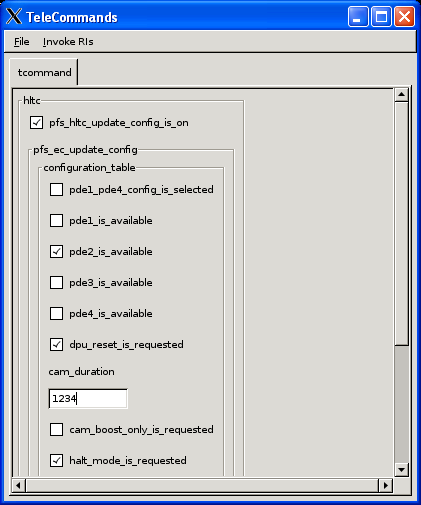
\includegraphics[width=0.55\textwidth]{imgs/gui1}
\caption{Automatically generated GUIs for TM/TCs}
\label{gui1}
\end{figure}

   \section{Automatic run-time monitoring of TM/TCs via MSCs}
Using the \texttt{tracer.py} and \texttt{tracerd.py} utilities, the automatically generated 
TASTE GUIs message exchanges (i.e. telemetry and telecommands) can be monitored in real-time,
via the freely available PragmaDev MSC Tracer\footnote{MSC Tracer available at \url{http://www.pragmadev.com/product/tracing.html}.}.
This allows for direct and simple monitoring of the communications
channels between the TASTE GUIs and the main applications (see figure \ref{msc}).

\begin{figure}
\centering
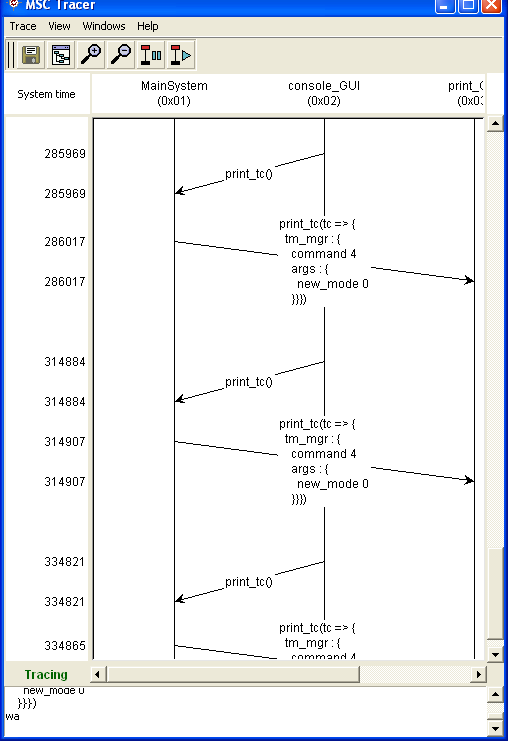
\includegraphics[width=0.65\textwidth]{imgs/msc}
\caption{Automatic monitoring of TM/TCs via MSC Tracer}
\label{msc}
\end{figure}

   \section{Automatic Python test scripts}
Testing the (usually complex) logic inside space systems requires big regression checking suites. TASTE tools automatically create Python bridges that offer direct access to the contents of the ASN.1 parameters, as well as direct runtime access to the TM/TCs offered by the system.

All that the user needs to do to create his set of regression checks, is to write simple Python scripts, that exercise any behavioural aspect of the system. For example, a scenario like this: 


\begin{quote}
when I send a TC with value X in param Y, \\
then I expect a TM after a max waiting of Z seconds, \\
with the value K in the incoming param L
\end{quote} 

...can be expressed in less than 10 lines of Python code, with an order of magnitude less work than the corresponding C code.

\subsection{Recording of real-time usage into a Python script}
The {\tt tracerd.py} tool (or, equivalently, the corresponding GUI version, {\tt tracerGUI.py}) allows recording of the exchange of TM/TCs into MSC files. Subsequently, the {\tt msc2py} tool allows conversion of the recorded MSC data into a Python script, that will exercise the scenario at runtime (i.e. send the recorded TCs, and verify the incoming TMs against the recorded TM responses). This is an easy way to automatically create Python test scripts, reproducing specific scenarios. 

See the relevant video \footnote{Use Videolan to play the video: get it from \url{http://www.videolan.org}} demonstrating the usage of {\tt tracerGUI.py} and {\tt msc2py} from \url{http://semantix.gr/assert/Msc.flv}.

\begin{figure}[!h]
\centering
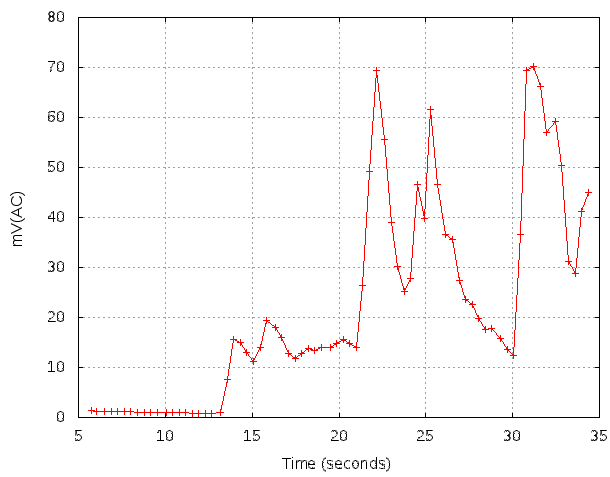
\includegraphics[width=0.75\textwidth]{imgs/gui2}
\caption{Graphical monitoring of telemetry data in real-time}
\label{gui2}
\end{figure}


\section{Automatic integration with SQL databases}

By using ASN.1 as the basis of all types in all subsystems, TASTE allows for automatic serialization/deserialization of any type instance inside SQL databases. The TASTE developer does not need to write any code to achieve this; any instances can be serialized to automatically created database tables, that mirror the semantic content of the ASN.1 definitions, and also express -  to the maximum possible extent\footnote{To the extent that the underlying database engine supports them, ASN.1 constraints (integer ranges, etc) are mapped to SQL constraints.} the corresponding ASN.1 constraints.

TASTE currently supports automatic database access for the Python language, via the SQLAlchemy Object Relational Mapper\footnote{SQLAlchemy, the Python SQL Toolkit and Object Relational Mapper: \url{http://www.sqlalchemy.org}.}. This means that any database engine can be used (tested so far: PostgreSQL, MySQL, SQLite), and that e.g. Python test cases can record and re-send Telemetries and Telecommands, without the user having to write any DB-specific code.

\section{Acknowledgements - who did TASTE}
TASTE is a complex tool-chain made of a number of components that were developed by various people and various companies. This section contains a list of TASTE authors and contributors. It may not be exhaustive, as many partners are regularly contributing to the toolchain development. 

\begin{enumerate}
     \item
	ESA (European Space Agency) is responsible for TASTE technical lead and management, and for the buildsupport, polyorb-hi-c, rtems port, tastegui tools, etc.
    \item
	SEMANTIX is responsible for the TASTE disribution, the design and implementation of the data modelling tools based on ASN.1, the integration, validation and release of the TASTE virtual machine, the vhdl, msc, gnuplot support, etc.
    \item
	ELLIDISS is responsible for the development of the interface and deployment view GUI editors.
    \item
	ISAE is responsible for the polyorb-hi-ada and ocarina tools.
    \item
	TELECOM-PARISTECH is the original developer of the ocarina and polyorb tools
    \item
	UPM is developing the gnatforleon runtime (Ada runtime for LEON processors), the original AADL to MAST convertor, and some drivers (serial, spacewire) for the Ada runtime.
    \item
	PRAGMADEV provides the free MSC tracer that can be used to trace communication within the blocks of the system.
    \item
	ASSERT partners provided inputs to the overal process (see ASSERT website for more information)
\end{enumerate}


\chapter{\taste concepts}
\section{The TASTE steps in building an application}
\label{assertProcess}
\begin{figure}[ht]
\centering
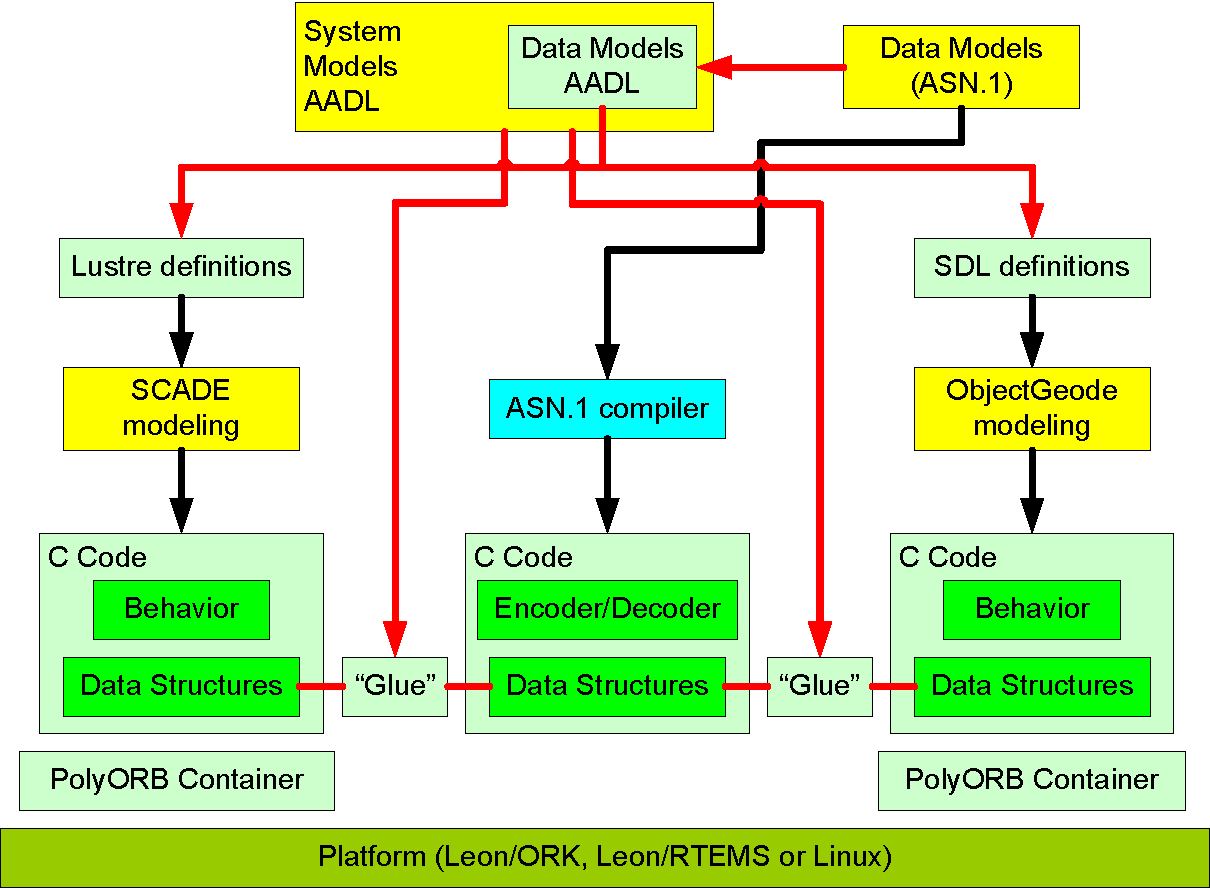
\includegraphics[width=13cm]{imgs/diagram}
\caption{Data Modeling with ASN.1}
\label{diagram}
\end{figure}
Figure \ref{diagram} displays a high level view of how TASTE integrates the individual
pieces of an overall system. The yellow blocks depict stages where manual labour
is required, and the green ones depict machine-generated entities.
\begin{enumerate}
\item The process begins with manual specification of the data models for the messages exchanged between
subsystems (TASTE "Functions"). This is where details about types and constraints of the exchanged messages
are specified. To be usable from within the system AADL specifications, 
these message definitions are translated into AADL data definitions. 
These definitions are in turn used by the system designer (the one doing the high-level
interface modeling): they are referenced inside the high level design of the system, when describing
the system's interfaces. The Interface View in AADL explicitely describes the interfaces,
in terms of the available ASN.1 types.
\item \label{asn2dataModel} The actual functional modeling of subsystems is next - but before it begins,
the exchanged messages' descriptions are read by TASTE, and semantically
equivalent definitions of the data messages are automatically created for each modeling tool's language
(e.g. Lustre definitions for SCADE modeling, Simulink definitions for MATLAB/Simulink modeling, etc).
This way, the teams building the individual subsystems are secure in their knowledge that their message representations
are semantically equivalent and that no loss of information can occur at Interface borders.
\item Functional modeling is then done for the individual subsystems. The modeling uses the
data definitions as they were generated in step \ref{asn2dataModel}. In fact, the modelling 
has absolutely no work to do in terms of interface specification: the interfaces are 100\%
automatically generated by TASTE, in so-called "skeleton" projects. If the interface view
specifies that a Function is written in SCADE, a SCADE skeleton will be generated by TASTE,
and the user fills-in the "meat" of the calculation. If the interface view specifies that a
Function is written in C, then TASTE generates a .h/.c declaration/definition of the interface,
and the user just fills-in the details. Etc.
\item When functional modeling is completed, the modeling tools' code generators are put to use,
and C code is generated (this step does not exist if the Function is manually written in C or Ada). 
Modeling tools generate code in different ways; even though (thanks to
step \ref{asn2dataModel}) the data structures of the generated code across different modeling tools
are carrying semantically equivalent information, the actual code
generated cannot interoperate as is; error-prone manual labour is required to ``glue'' the pieces together.
This is the source of many problems\footnote{Lost satellites being one
of them.}, which is why ASN.1 is used in TASTE: by placing it as the center of a star formation 
amongst all modeling tools, the ``glue-ing'' can be done automatically.
\item TASTE automatically invokes the ASN.1 compiler to create encoders and decoders for the messages.
\item TASTE automatically creates ``glue'' code that maps (at runtime) the data from
the data structures generated by the modeling tools to/from the data structures generated by the 
ASN.1 compiler.
\item Code from the ASN.1 compiler, code from the modeling tools and ``glue'' code are compiled
together inside PolyORB-Hi containers, generated by Ocarina.
\item The generated binaries (OpenRavenscar / RTEMS / Linux) are executed.
\end{enumerate}
   \section{\taste guidelines}
   \taste aims at providing a Component-Based Software Engineering approach
   by defining a methodology that builds systems \textit{correct by
   construction}: users define the functional aspects of the system using
   \textit{containers}, \textit{functions}, \textit{interfaces} and describe their
   allocation on the hardware (using a so-called \textit{Deployment view}).

   Using this information, the \taste toolchain generates the code that is
   responsible for component execution. It instantiates system resources (data,
   mutexes, tasks, etc.) and allocates software on them. As is the case for every 
   real-time system, the generated systems enforce a computational model as well as several
   restrictions.

   The computational model that is checked is the \textit{Ravenscar} computation
   model. So, every function of the system must comply with these restrictions:
   \begin{enumerate}
      \item
         Tasks are scheduled using a FIFO via a priority scheduling
         algorithm.

      \item
         The locking policy uses the ceiling protocol.

      \item
         No blocking operations are allowed in protected functions
      \item
         The following restrictions as defined in the Ada compiler must also be
         applied to any functions that are written in other languages:
         \begin{itemize}
            \item
                No\_Abort\_Statements
            \item
                No\_Dynamic\_Attachment
            \item
                No\_Dynamic\_Priorities
            \item
                No\_Implicit\_Heap\_Allocations
            \item
                No\_Local\_Protected\_Objects
            \item
                No\_Local\_Timing\_Events
            \item
                No\_Protected\_Type\_Allocators
            \item
                No\_Relative\_Delay
            \item
                No\_Requeue\_Statements
            \item
                No\_Select\_Statements
            \item
                No\_Specific\_Termination\_Handlers
            \item
                No\_Task\_Allocators
            \item
                No\_Task\_Hierarchy
            \item
                No\_Task\_Termination
            \item
                Simple\_Barriers
            \item
                Max\_Entry\_Queue\_Length => 1
            \item
                Max\_Protected\_Entries  => 1
            \item
                Max\_Task\_Entries       => 0
            \item
                No\_Dependence => Ada.Asynchronous\_Task\_Control
            \item
                No\_Dependence => Ada.Calendar
            \item
                No\_Dependence => Ada.Execution\_Time.Group\_Budget
            \item
                No\_Dependence => Ada.Execution\_Time.Timers
            \item
                No\_Dependence => Ada.Task\_Attributes
          \end{itemize}
   \end{enumerate}

   In addition, the following restrictions must also be enforced by each
   component used in \taste programs:
   \begin{enumerate}
      \item
         No controlled types. In Ada, this is provided by \texttt{pragma Restrictions (No\_Dependence => Ada.Finalization);}

      \item
         No implicit dependency on object oriented features.
         Ada provides this restriction with
         \texttt{pragma Restrictions (No\_Dependence => Ada.Streams)}

      \item
         No exception handler shall be defined.
         Ada provides this restriction with:
         \texttt{pragma Restrictions (No\_Exception\_Handlers)}

      \item
         No unconstrained objects, including arrays - and forbidden
         string concatenation.
         Ada provides this restriction with:
         \texttt{pragma Restrictions (No\_Secondary\_Stack)}

      \item
         Do not use allocation. Ada provides this restriction with
         \texttt{pragma Restrictions (No\_Allocators)}
      \item
         All access/references to variables must be explicitly typed.
         Ada check that using the restriction:
         \texttt{pragma Restrictions (No\_Unchecked\_Access)}
      \item
         Avoid explicit dispatch. Ada provides this features with
         \texttt{pragma Restrictions (No\_Dispatch)}
      \item
         Do not use input/output mechanisms.
         Ada provides this feature/restriction with:
         \texttt{pragma Restrictions (No\_IO)}
      \item
         Do not use recursion. Ada provides this feature with:
         \texttt{pragma Restrictions (No\_Recursion)}
      \item
         As for allocation, memory deallocation must be checked.
         This is provided in Ada with
         \texttt{pragma Restrictions (No\_Unchecked\_Deallocation)}
   \end{enumerate}


   \section{Main components}
   \taste is centered around the following elements:
   \begin{enumerate}
      \item
         The \textbf{Data View} describes the data definitions of your system. It
         defines data types using the ASN.1 standard\footnote{Read about ASN.1 on \url{http://en.wikipedia.org/wiki/ASN.1}}.
      \item
         The \textbf{Interface View} details the system from a purely functional
         point of view. This view describes the functions performed by the
         system and the data types that they handle. Data associated with the
         functions rely on the \textbf{Data View} definitions.
      \item
         The \textbf{Deployment View} defines how system functions are bound on
         the hardware. It defines the underlying architecture (processors,
         devices, memories, etc.) and allocates each function on these hardware
         components.
      \item
         The \textbf{Concurrency View} represents software and hardware aspects
         of the system. It contains tasks, data and communication between system
         artifacts (tasks, processes, subprograms, etc.). The
         \textbf{concurrency view} is automatically generated from the
         \textbf{interface view} and the \textbf{deployment view} by the
         \textbf{buildsupport} tool (see section \ref{section-buildsupport}).
         Thus, all the mapping rules that transforms system interfaces and deployment
         information are included in this tool that automatically generates a
         complete description of the system.

         Finally, the \textbf{Concurrency view} provides a complete view of the
         system, giving the ability to analyze it using validation tools.
         The \textbf{TASTE-CV} tool \ref{section-taste-toolsuite} provides such functionnality, linking the
         concurrency view with schedulability analysis tool.
   \end{enumerate}

   \section{Development process overview}
   Once designers have specified the different views (\textbf{Data}, \textbf{Interface},
   and \textbf{Deployment}), the \taste tools automatically generate code
   that implements the system. In particular, they generate data definitions in 
   whatever language is used to describe the functionality of each system
   (SCADE models, Simulink models, C header files, Ada .ads files, etc) as well
   as ``skeleton'' projects (.xscade files, .mdl files, .c/.adb files, etc)
   that include the formal specifications of interfaces, with empty implementations.
   The tools also create the code that connects function interfaces with their callers
   (they can do that, because the Interface View includes these connections).
   Finally, they produce the code required to execute the functions on top of 
   Real-Time operating systems (such as RT-Linux, RTEMS, etc.).

   Finally, these code generators auto-configure and deploy the system so that
   you don't have to write additional code and introduce potential errors.
   Network addresses, drivers and all other deployment code is automatically
   generated.

   The whole process is illustrated in the figure below: the user defines the
   \textbf{Data View}, the \textbf{Interface View} and the \textbf{Deployment
   View}. Then, appropriate tools (code generators) automatically produce data
   handling functions, interaction code with the functional code as well as
   deployment and configuration code to execute the system on top of an RTOS.

   \centerline{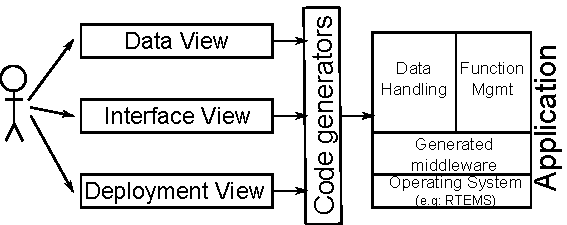
\epsfig{file=imgs/development-process.pdf,width=.90\textwidth}}

   As a result, this approach creates systems that are correct by construction.
   By generating the system from a high-level description, we can make several
   validation and/or verification and ensure designers' requirements.

   \section{Definitions}
   \begin{itemize}
      \item
         The \textbf{Concurrency View} is automatically generated through the
         \textbf{vertical transformation} process. It creates resources (tasks,
         mutexes, etc.) of the system and associates functions to them.
      \item
         The \textbf{Data View} contains the definition of all data types used
         in the functions' interfaces, using the ASN.1 notation.
      \item
         The \textbf{Interface View} defines the functions of your system with
         their respective interfaces and data ports.
      \item
         A \textbf{periodic interface} is executed according to a predefined period. It
         also has other properties, such as the deadline.
      \item
         A \textbf{protected interface} is executed exclusively by one entity, meaning that
         only one thread can be executing this function at the same time.
      \item
         A \textbf{sporadic interface} is triggered by a reception of an event. The time
         between two events is bounded and is specified with a value known as
         the Minimul Inter-Arrival Time (MIAT).
      \item
         An \textbf{unprotected interface} may be executed concurrently by different 
         entities.
   \end{itemize}

   \section{Modeling rules}
   You have four operation kinds (that correspond to the \aadl property:
   \begin{enumerate}
      \item
         Periodic
      \item
         Sporadic
      \item
         Protected/unprotected
   \end{enumerate}

   A function can contain any mix of the following categories of provided interfaces (PI):
   \begin{enumerate}
         \item \textbf{Sporadic and Cyclic}
            \begin{itemize}
               \item
                  Sporadic can't have OUT params, since they are asynchronous
                  (caller doesn't wait for them to return, so no results can be
                  returned from their invocation).
               \item
                  Each Sporadic/Cyclic PI gets one thread. They DONT run in the calling thread context.
               \item
                  There is automatic mutual exclusion between all PIs that are Sporadic and/or Cyclic 
                  inside the same Function, via a protected object. To be more exact, Sporadic and 
                  Cyclic PIs get their own threads, but when they are called and need to execute their 
                  actual implementations (user code), the actual user code call is done from inside 
                  a protected object - and thus, mutual exclusion takes place 
                  (only one Sporadic/Cyclic can be active at any time). 
               \item
                  Cyclic don't have IN or OUT params, they are called periodically
               \item
                  Sporadic can only have ONE IN param, carrying all the data they need.
               \item
                  Sporadic can in fact be considered a special kind of Cyclic,
                  since they have MIAT (Minimum Inter-Arrival Time) which is enforced at run-time.
            \end{itemize}
         \item \textbf{Protected and Unprotected}
            \begin{itemize}
               \item
                  run in the calling thread context
               \item
                  can have multiple IN and OUT params
               \item
                  are synchronous, that is the calling thread waits 
                  for them to return (since they have OUT values 
                  that it wants to read).
               \item
                  Protected PIs use a standard mechanism (Protected Object when compiling with the Ada runtime,
                  and semaphore otherwise) to 
                  guarantee mutual exclusion between a Function'
                  s protected PIs, so you use them whenever the 
                  Function's PIs share state and would have issues 
                  with multiple calling threads entering two or more 
                  of them simultaneously and messing up the shared state.
               \item
                  Unprotected can read/write anything they want, so they 
                  allow the calling context to enter at will. 
               \item
                  Protected and Unprotected can co-exist inside a Function 
                  (since you may have functionality that has no state-dependencies). 
            \end{itemize}

         \end{enumerate}

   \section{Symbol clashing}
	The TASTE code generators read the models of the system (Data models, 
	interface/deployment models, etc) and create a lot of "boilerplate" code
	(in C/Ada/etc) that would be otherwise written manually. 

	This implies that you must be careful in your models, so that you don't use reserved
	keywords - for example, you can't name a field of your types {\tt "else"},
	since {\t else} is a reserved keyword in many languages and tools.

	The complete list of forbidden keywords exists in {\tt commonPy/asnParser.py},
	and is called {\tt g\_invalidKeywords}. Feel free to enhance it with 
	any other keywords you'd like TASTE to stop you from using (i.e. detect
	usage of forbidden symbols during code-generation and abort).

\chapter{Overview of the \taste toolset}
   \section{Labassert}
   \textbf{Labassert} is a graphical tool developed by \textsc{Ellidiss Technologies} to
   edit the \textbf{Interface} and \textbf{Deployment} views. Labassert works on
   Windows and Linux.

   However, this tool is now considered as deprecated and is replaced by three
   programs : \textbf{TASTE-IV}, \textbf{TASTE-DV} and \textbf{TASTE-CV}.

   \section{TASTE toolset (TASTE-IV, TASTE-DV and TASTE-CV)}
   \label{section-taste-toolsuite}
   \textbf{TASTE-IV} is the tool used to edit the interface view of your system:
   it provides functionnalities to describe system functions, their
   parameters and in which language they are implemented. \textbf{TASTE-DV} is
   the editor for the deployment view, providing functionnalities to describe
   how system functions are allocated to processing resources (CPU, network,
   etc.). Finally, \textbf{TASTE-CV} is the concurrency view editor. It is used
   to perform schedulability analysis and simulates system execution, detecting
   potential system errors that can be risen at run-time (deadlocks, etc.).


   \section{ASN.1 generators}
   \textbf{ASN.1 generators} consist in tools that creates data types and run-time data translation
   "bridges" (between e.g. SCADE/KCG code and Simulink/RTW code) from the ASN.1 type descriptions. 
   These tools are developed by \textsc{Semantix Information Technologies}.

   \section{Ocarina}
   \textbf{Ocarina} is a toolchain to manipulate \aadl models. It runs on Windows, Linux
   and Mac OS X and proposes code generation features that produce code that
   targets real-time middleware such as PolyORB.

   \section{PolyORB-HI}
   \textbf{PolyORB-HI} is the middleware that interfaces generated code from \aadl models
   to the RTOS. It maps the primitives of the generated code to the ones offered by the
   operating system, in order to ensure their integration. PolyORB-HI provides
   the following services to the generated code:
   \begin{itemize}
      \item
         \textbf{Tasking}: handle tasks according to their requirements (period,
         deadline, etc.)
      \item
         \textbf{Data}: define types and locking primitives
      \item
         \textbf{Communication}: send/receive data on the local application and
         send them to the other nodes of the distributed system.
      \item
         \textbf{Device Drivers}: interact with devices when a connection uses a
         specific bus.
   \end{itemize}

   There are two versions of PolyORB-HI: one for Ada and one for C. They are
   described in the following paragraphs.

      \subsection{Ada version}
      The Ada version can be used on top of Linux, RTEMS and Open Ravenscar
      Kernel (ORK). It enforces the Ravenscar profile and has been successfully
      tested on LEON and x86 targets.

      \subsection{C version}
      The C version can be used on top of Linux, RT-Linux, Maemo and RTEMS. It
      works on LEON, ARM, PowerPC and x86. It was successfully tested on native
      computers (x86 with Linux), LEON boards (with RTEMS), ARM (with DSLinux
      and Maemo).

   \section{Buildsupport}
   \label{section-buildsupport}
   Buildsupport provides several functionalities:
   \begin{enumerate}
      \item
         It generates the \textbf{concurrency view}
         from the \textbf{interface} and \textbf{deployment} views. The result is
         an \aadl models that is subsequently processed by Ocarina to generate and build the
         system in C or Ada.
      \item
         It creates skeletons (for each Function's target environment, e.g. .xscade files 
         for SCADE Functions, .h/.c files for C Functions, .ads/.adb for Ada Functions, etc)
         that include the complete specifications of interfaces, with empty implementations.
   \end{enumerate}
   
   This part assumes that we have a description of all Archetypes, meaning how we convert the interface and
   deployment view into a concurrency view that describe tasking concerns. It
   means that this tool contain all relevant information to map a
   cyclic/sporadic/protected/unprotected interface into thread and data.


   \boxfixme{TO BE COMPLETED BY MAXIME}

   \section{Orchestrator}
   The orchestrator is a program that automates the build process. It
   takes as input the data view, the interface view, the deployment view, as well
   as the complete Functional code (i.e. the filled-in skeletons), and then
   calls each tool (buildsupport, ocarina, compilation scripts and so on). As a
   result, the Orchestrator produces the final binaries that correspond to the
   system implementation.

   The tool is maintained by \textsc{Semantix Information Technologies}.

   The process that is followed by the orchestrator and the way it calls other
   tools is illustrated in the following figure.

   \centerline{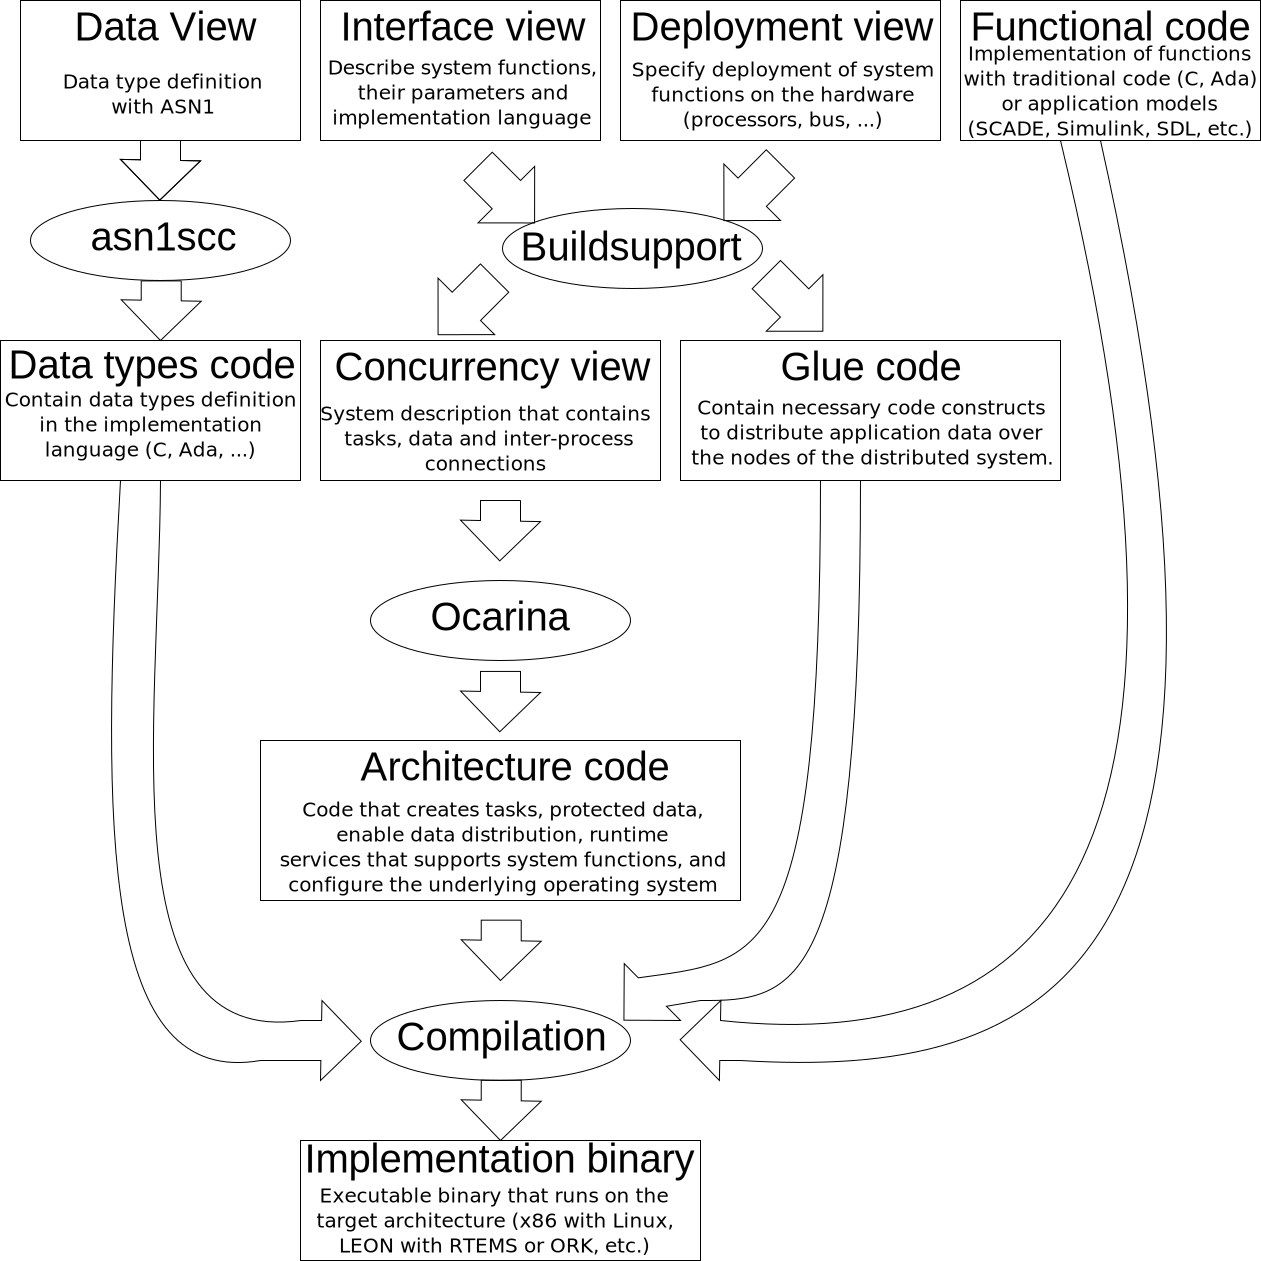
\epsfig{file=imgs/orchestrator-process.pdf,width=.90\textwidth}}

   \section{TASTE GUI}
   The \taste GUI is a program which purpose is to assist the system designer in
   the use of the different tools of \taste. It provides a convenient interface
   to design the different views of your system (data, interface and
   deployment).

   The TASTE GUI is available in the \taste virtual machine (VM), as well as an
   independent package. An example of the interface is shown in the following
   picture.

   \centerline{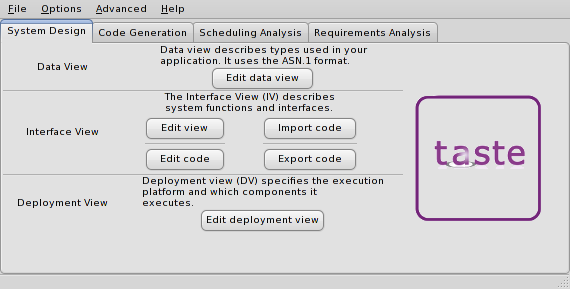
\epsfig{file=imgs/tastegui-main.pdf,width=.90\textwidth}}

   The program let you define the view of your system but also let you edit
   their definition using a text editor. Finally, it provides some
   functionnalities to deploy generated applications and choose the runtime used
   (PolyORB-HI-C, PolyORB-HI-Ada, etc.).

   \section{TASTE daemon (\textit{tasted})}
   The TASTE daemon is a program designed to ease the execution of generated
   applications. It was especially designed to interact with TASTE GUI (as
   detailed in section \ref{tastegui-tasted}) : once
   system designers have successfully built their systems, they can
   automatically execute them on boards.
   As the TASTE toolset can produced applications for systems with
   different architectures and requirements, it is sometimes difficult to deploy
   them altogether. The TASTE daemon aims at facilitate this deployment and
   execution step.

   The TASTE daemon runs on a machine (potentially the same machine as the host
   development) and listen for incoming request. Then, the TASTE GUI tool sends
   generated applications and receives execution output from the daemon.

   \centerline{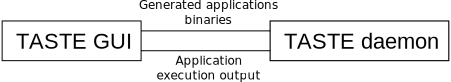
\epsfig{file=imgs/tastegui-tasted.pdf,width=.90\textwidth}}

   \section{Additional tools}

   The \taste process relies on third-party tools to either model
 functions; or RTOS to execute the final systems. It is the user
 responsibility to get a valid license and install
 them. Chapter~\ref{do_packaging} illustrates how to import your
 models and the code generated from this tools in the \taste
 toolchain.

The \taste toolchain supports the following tools:

\begin{itemize}
\item Simulink / Real Time Workshop v7.0
\item Scade / KCG v6.1.2
\item SDL tools ObjectGeode v4.2.1 and PragmaDev RTDS v4.12
\end{itemize}

In addition, the \taste toolchain can generate binaries for the
 following platforms:

\begin{itemize}
\item RTEMS from OAR Technologies, version 4.8.0,
\item ORK+ from the Universidad Polit\'ecnica de Madrid, version 2.1.1,
\item Linux and most POSIX-compatible variants, including embedded ones.
\end{itemize}

\chapter{Installation and upgrade of the TASTE toolchain}
There are two ways to use the TASTE toolchain : a regular installation on a
Linux system and use of a virtual machine. The virtual machine system provides a
complete environment with a predefined Linux installation that contains
everything. The installation on your Linux system gives you the ability to use
the toolchain with your day-to-day environment. It is more convenient in many
ways but the TASTE developpers does not provide official support on such
installation.

Support is provided only for users that are using the tools within the VM.
Indeed, the use of the same architecture ease bug detection and provide a
similar environment for both users and developers, and so, is more convenient to
reproduce bugs related to the toolchain (and not environment of the user).



   \section{Installation of the virtual machine}
   The Virtual Machine system needs to install a software able to execute VMWare
   image. For that purpose, you can download VMWare Player at the following
   address: \url{http://www.vmware.com/products/player}.

   Then, once installed, you need to download the TASTE virtual machine
   available at this address:
   \url{http://download.tuxfamily.org/taste/taste-vm.tar.gz}.

   Finally, launch VMWare Player, open the TASTE VM so that you can start to use
   the tools in the configured environment.


   \section{Installation on your own Linux distribution}
      \subsection{Distributions}
      At this time, we support the following distributions:
      \begin{itemize}
         \item
            Debian
         \item
            Ubuntu
         \item
            Mandriva
      \end{itemize}

      \subsection{Using the installation script}
      We provide an installation script that ease the installation and deployment
      of our tools. You can find the installation program at
      \url{http://download.tuxfamily.org/taste/taste-installer.sh}.

      The installation program requires you have the program/package
      \texttt{dialog} installed on your system. If it is not installed, use the
      package manager of your distribution to install it. Then, invoke the
      program, you would see the following screen.

     \centerline{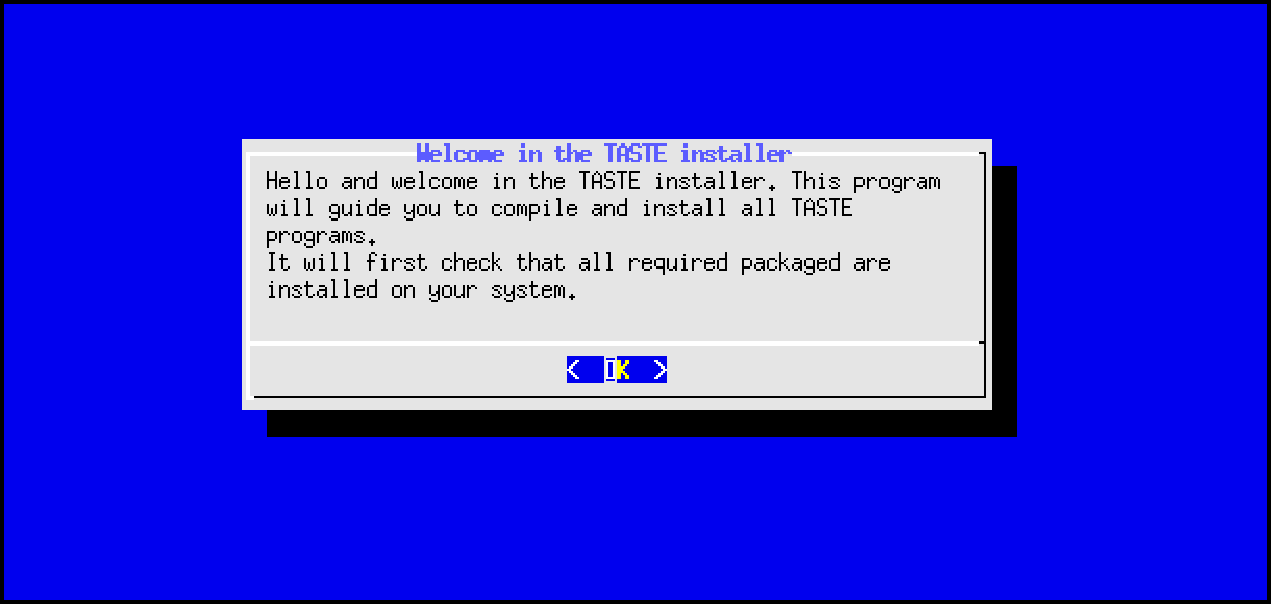
\epsfig{file=imgs/installer1.pdf,width=.70\textwidth}}

     At first, you are asked to provide the installation directory. This
     directory must exist on your system and you must be allowed to write in it.

     Then, you can choose which packages to install on your system. We advise
     you to choose and install every TASTE tools.

     \centerline{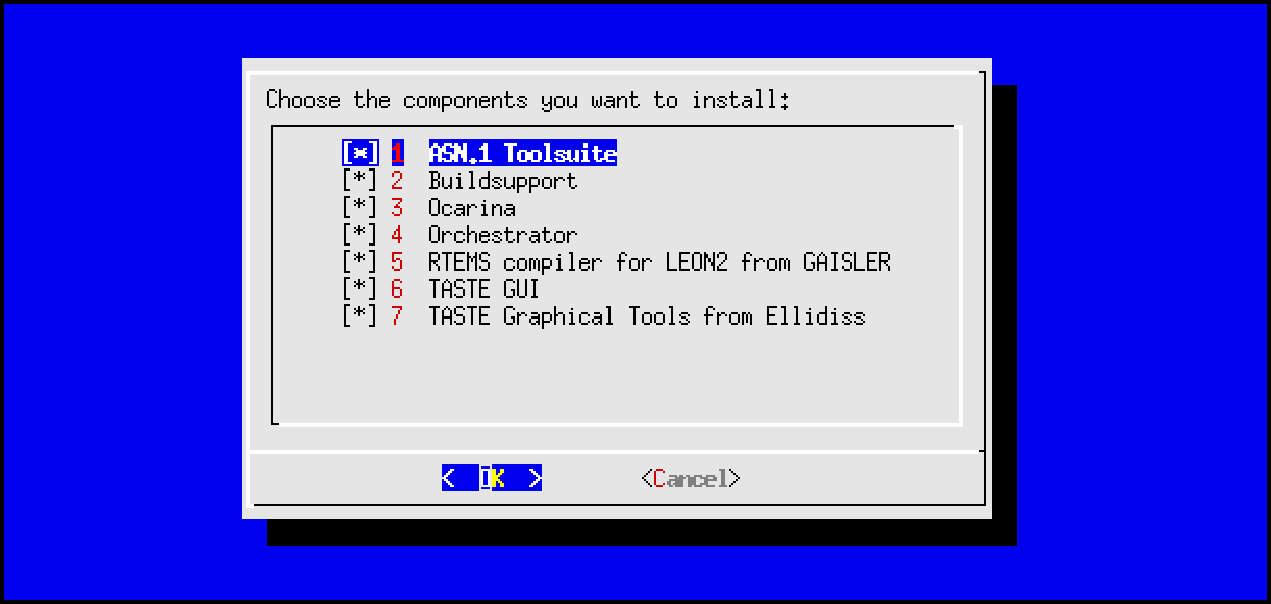
\epsfig{file=imgs/installer2.pdf,width=.70\textwidth}}

     As the TASTE graphical tools are not directly available on the internet and
     require you download them manually on Ellidiss website
     (\url{http://www.ellidiss.com}), you are asked to provide the archive file
     of the program of you want to install them. To do so, a file dialog chooser
     will ask you to provide the location of the TASTE tools, as shown in the
     following picture.

     \centerline{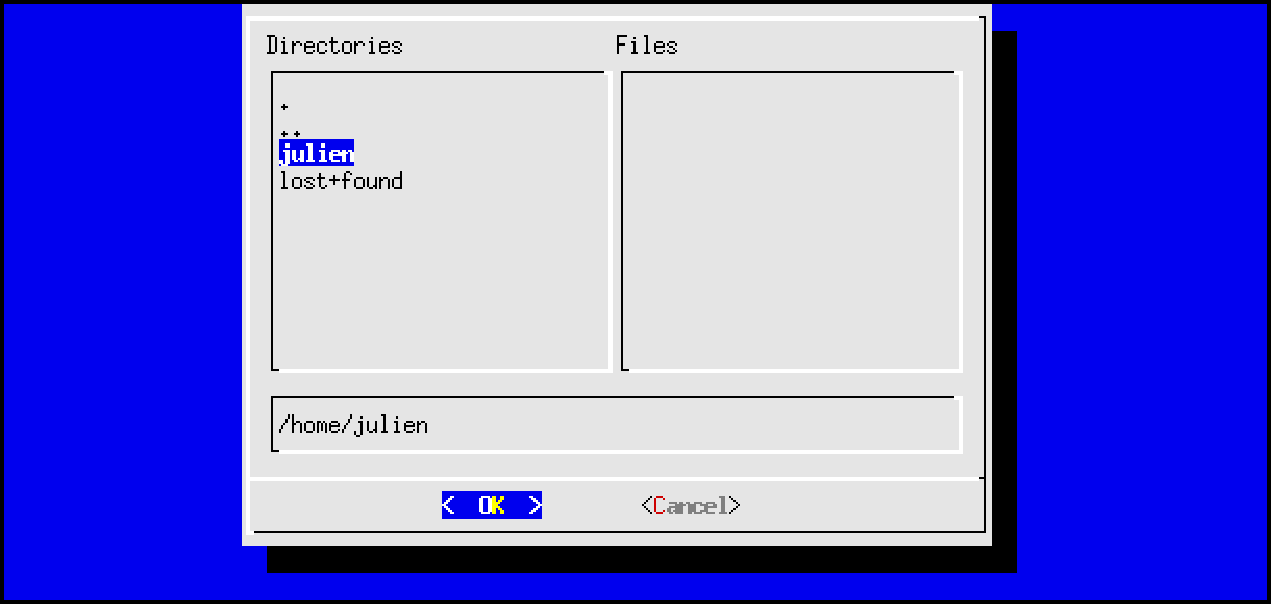
\epsfig{file=imgs/installer4.pdf,width=.70\textwidth}}

     Then, the installation process starts, download software archive on the
     internet, compile and install them.

     \centerline{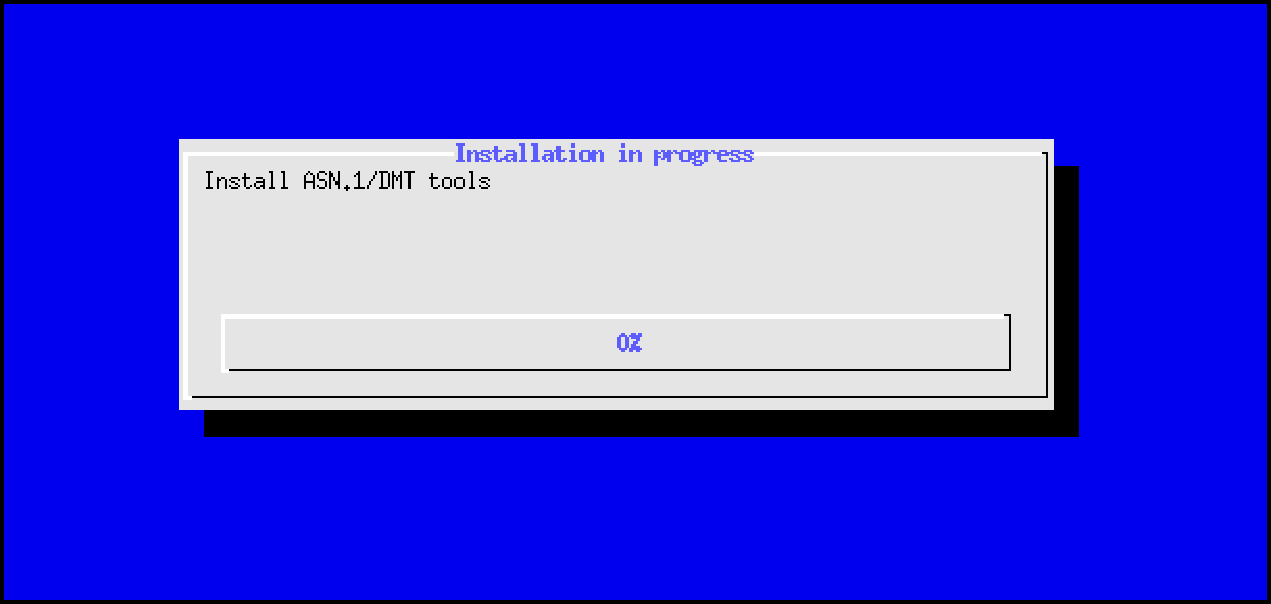
\epsfig{file=imgs/installer5.pdf,width=.70\textwidth}}

     Finally, if everything runs fine, the following screen would appear. If
     some error was raised, a dialog error will appear. In that case, you can
     see the installation log in the file \texttt{/tmp/taste-installer-log}.

     \centerline{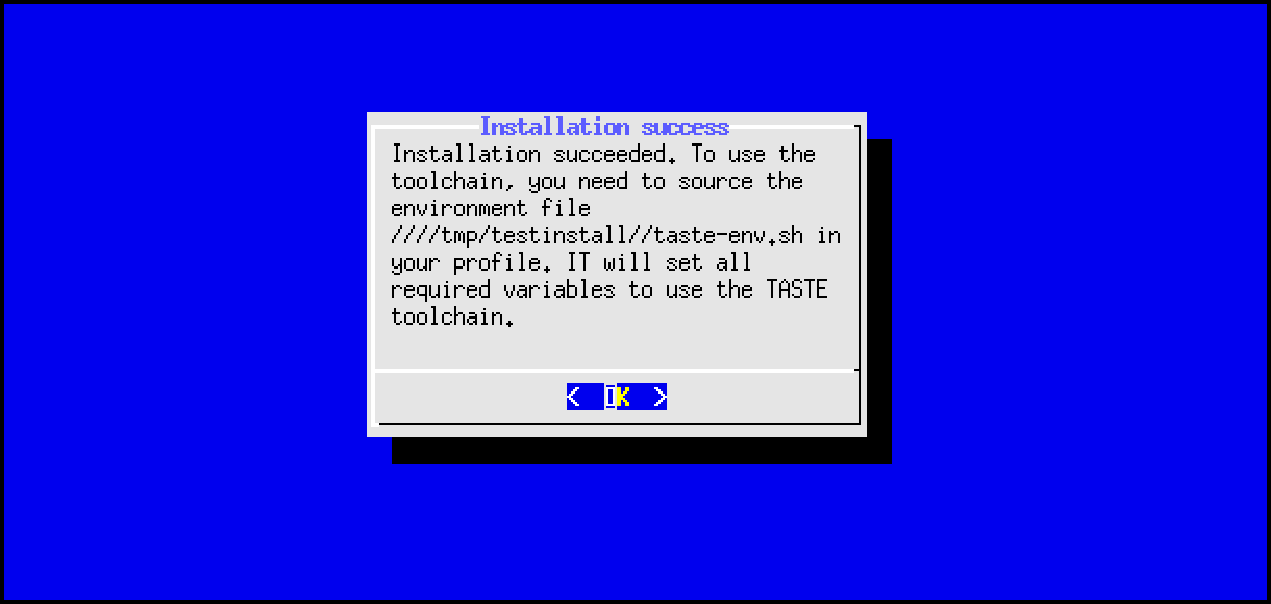
\epsfig{file=imgs/installer6.pdf,width=.70\textwidth}}

     Finally, TASTE tools requires that you defined some environment variables.
     The installer automates this process by creating a shell-script that
     contains all new environment variables. It is located in the installation
     directory, with the name \texttt{taste-env.sh}. So, if you installed the
     tools under the directory \texttt{/home/user/local/}, you are required to
     use the file \texttt{/home/user/local/taste-env.sh}. This can be done
     automatically by adding the following line in your shell configuration
     file:
     \begin{verbatim}
source /path/to/installation/taste-env.sh
     \end{verbatim}

     Assuming you installed the tools in \texttt{/home/user/local/}, you will
     add the following line in your shell configuration file (for example
     \texttt{\$HOME/.bashrc}):
     \begin{verbatim}
source /home/user/local/taste-env.sh
     \end{verbatim}





   \section{Upgrade within the virtual machine}
   To upgrade the tools to the latest version within the virtual machine, invoke
   the script \texttt{UPDATE-TASTE.sh}. Open a terminal and invoke the command.
   Once called, it downloads the latest version of each tool and install them in
   their appropriate directory.


   \section{Upgrade on your own Linux distribution}
   If you want to upgrade the tools on your own installation, you need to run
   the installation program again. Fortunately, the installation program is
   already installed when you run it for the first time. In that case, you just
   have to invoke the command \texttt{taste-installer} on your system. It will
   restart the installation program and will use the installation directory you
   used at installation time to upgrade the tools.


\chapter{Using ASN.1}
ASN.1 is a standardized notation to represent data types. An overview of this
standard can be found on
\url{http://www.itu.int/ITU-T/asn1/introduction/index.htm}. For readers that are
interested in ASN.1 and want to learn the language, a tutorial can be found here: 
\url{http://www.obj-sys.com/asn1tutorial/asn1only.html}.

All data types exchanged between Function interfaces are described using ASN.1.
Data types definitions constitute the \textbf{Data View}. These types are
then used by function interfaces, to specify the parameter types in a 
standardized way. On the implementation side, code generators map 
the ASN.1 types into language-specific definitions (e.g. SCADE definitions, or
Simulink/RTW definitions, or Ada/C definitions, etc) and create
functions to exchange these types between different environments, regardless of their
specific characteristics (CPU models, endianness, word sizes, etc).

If you are not familiar with ASN.1, an easy way to get acquainted is to follow the
tutorial on \url{http://www.obj-sys.com/asn1tutorial/asn1only.html}.

\chapter{Using the graphical tool (The \textit{TASTE} toolsuite)}

   \section{The interface view: TASTE-IV}
   The interface view provides the ability to describe system functions with
   their provided and required interfaces. The picture below gives an example of
   the Interface View.

   \centerline{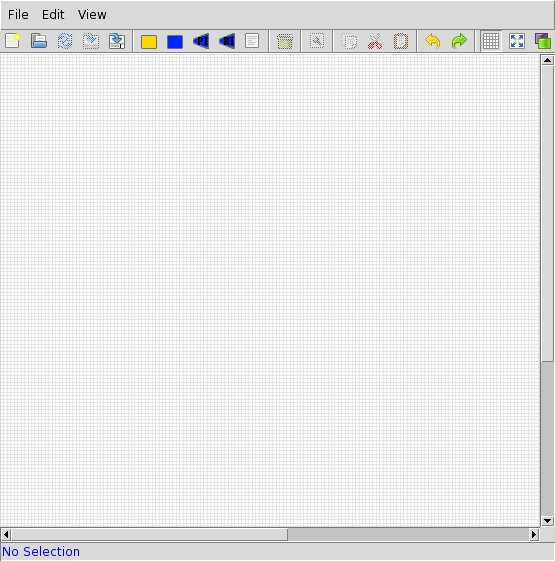
\epsfig{file=imgs/interface-view.pdf,width=.90\textwidth}}

   In the interface view, you define \textbf{containers}, \textbf{functions} and
   \textbf{provided/required interfaces}. The picture below illustrates the
   definition of two containers, each one containing one function. The function on
   the right uses a \textbf{Provided Interface} (\textbf{PI}) that is required
   by the function on the left. To describe that using the graphical interface,
   the interfaces are connected using a line and an arrow.

   \centerline{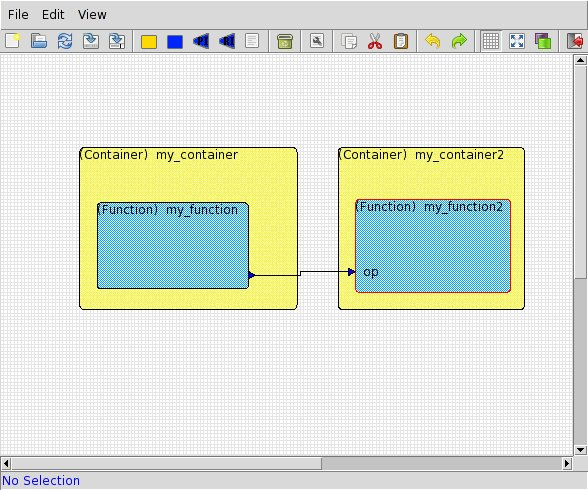
\epsfig{file=imgs/interface-view-two-functions2.pdf,width=.90\textwidth}}

   When you define an interface, you have to define its characteristics
   (periodic, sporadic, arrival time, etc.). For that, right-click on the
   \textbf{provided interface}, a menu will open. Choose \textbf{Properties}.

   \centerline{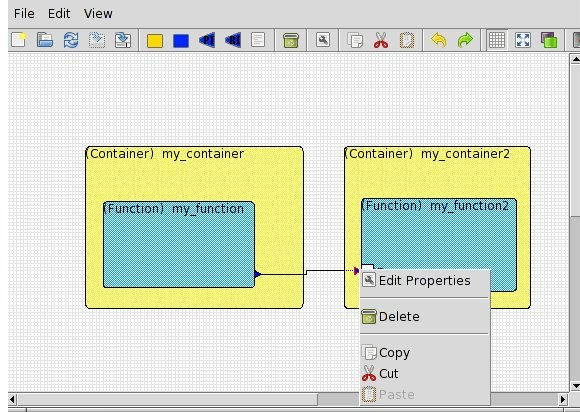
\epsfig{file=imgs/interface-view-pi-menu.pdf,width=.90\textwidth}}

   Then, a new window gives you the ability to define the characteristics of the
   \textbf{Provided Interface}, as shown in the following picture.

   \centerline{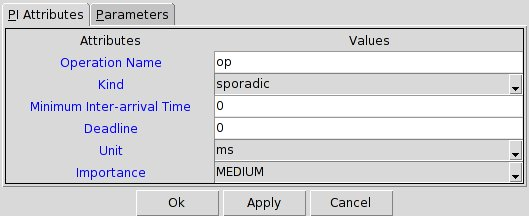
\epsfig{file=imgs/interface-view-pi-properties.pdf,width=.90\textwidth}}

   In the same window, you can also specify the data types of the \textbf{interface} 
   parameters, as illustrated in the following picture. Please also note that the types you
   specify in this window are defined in your \textbf{Data View} (your ASN.1 type definitions).

   \centerline{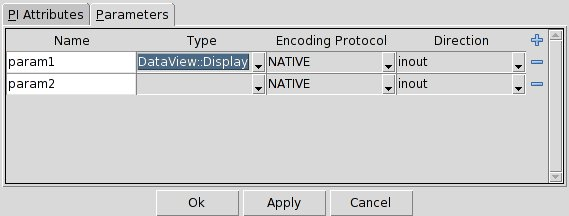
\epsfig{file=imgs/interface-view-pi-data2.pdf,width=.90\textwidth}}

   \section{The deployment view: TASTE-DV}

   The deployment view editor is a graphical tool that provides the ability to
   edit the \aadl definition of your architecture. A screenshot of the program follows: 

   \centerline{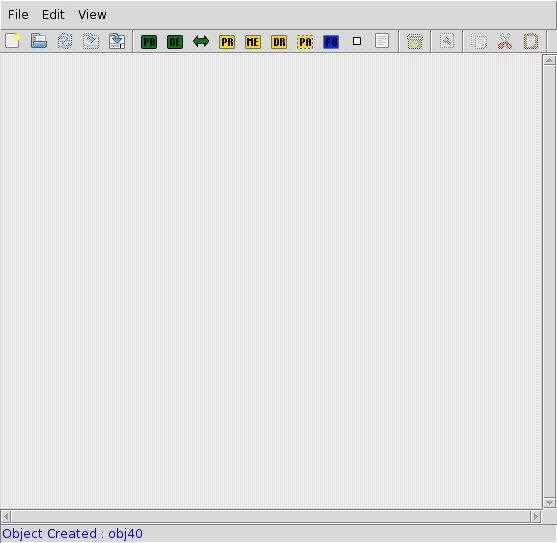
\epsfig{file=imgs/deploymentview.pdf,width=.90\textwidth}}

   You can then add hardware components in your architecture. It mainly
   consists of adding computer boards with their processors and memories.
   \textbf{Partitions} are then added, that will host the \textbf{functions} from
   your functional view. You can connect partitions (and thus, functions) by
   adding \textbf{buses} to your architecture and by connecting the processors
   with these buses.

   \centerline{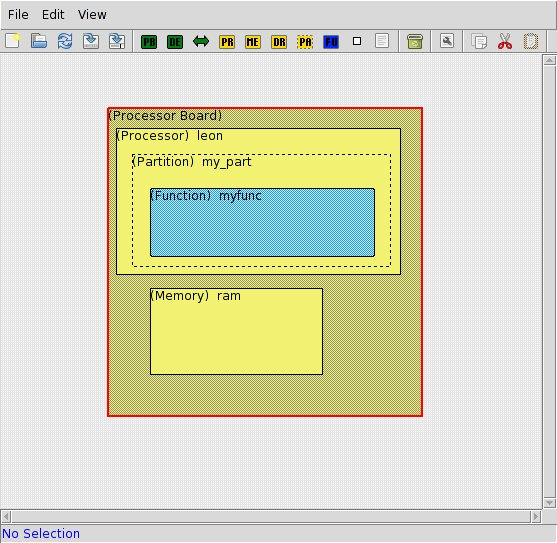
\epsfig{file=imgs/deploymentview-processor-board.pdf,width=.90\textwidth}}

   Note that when you add/specify a driver in the deployment view, it has to be
   configured. For example, for a network card that uses the TCP/IP protocol,
   you have to specify the IP address and the port used to receive incoming
   data. For serial port, you have to specify the corresponding device
   (\texttt{/dev/ttyS0}, etc.) as well as the speed of the port (115200 bauds,
   etc ..).

   This configuration is detailed in this documentation, within the PolyORB-HI-C
   and PolyORB-HI-Ada part. For PolyORB-HI-C, section \ref{polyorbhic-drivers}
   provides all required information.

   \section{The concurrency view: TASTE-CV}
   \textbf{TASTE-CV} has the ability to edit the concurrency view generated by buildsupport.
   It provides schedulability analysis functionalities to assess system
   scheduling feasability as well as scheduling simulation. Using this tool, we
   could be able to know if the deadlines of your tasks will be met and also
   inspect the behavior of your system, including its potential problems (such
   as deadlocks).

   To assess scheduling feasability, \textbf{TASTE-CV} embedds the
   \textbf{Cheddar} scheduling analyzer. It processes \aadl models and transform
   them into a suitable representation for Cheddar. The Cheddar output is based
   in scheduling theory and feasability tests. Readers interested in scheduling
   tests and scheduling theory could refer to articles listed on the official
   Cheddar website (see \ref{subsection-useful-programs} for web links).

   To simulate system scheduling, \textbf{TASTE-CV} relies on the \textbf{Marzhin}
   scheduling simulator. \textbf{Marzhin} shows the simulation of the execution
   of each tasks (running, waiting for a resource, sleeping, \ldots)
   as well as the state of shared data (locked, unlocked, \ldots).
  

   \subsection{Marzhin symbols}
   The following symbols are usedby \textbf{Marzhin} within the simulation
   window:
   \begin{itemize}
      \item 
         \texttt{\#} : Thread state none
      \item 
         \texttt{|} : Thread state running
      \item 
         \texttt{\_} : Thread state ready
      \item 
         \texttt{\~} : Thread state awaiting resource
      \item 
         \texttt{*} : Thread state awaiting return
      \item 
         \texttt{.} : Thread state suspended
      \item 
         \texttt{O} : Data state - occupied
      \item 
         \texttt{<} : Get resource
      \item 
         \texttt{>} : Release resource
      \item 
         \texttt{!} : Send Output or Subprogram Call
      \item 
         \texttt{1..9} : Queued events or call requests
      \item 
         \texttt{+} : More than 9 queued events or call requests
   \end{itemize}

   \subsection{Marzhin assumptions about system behavior}
   To simulate your system, \textbf{Marzhin} makes the following assumptions about the
   behavior of your system:
   \begin{itemize}
      \item
         An \aadl data component in the Concurrency View without specific
         properties is considered as protected with no specific protocol (no
         priority inversion).
      \item
         An \aadl data component can specifies the following protection
         mechanisms using the \texttt{Concurrency\_Control\_Protocol} property:
         \begin{enumerate}
            \item
               \textbf{IPCP} (value \texttt{Immediate\_Priority\_Ceiling\_Protocol})
            \item
               \textbf{PCP} (value  \texttt{Priority\_Ceiling\_Protocol})
         \end{enumerate}
      \item
         All \texttt{out} ports from the threads send data when the thread
         completes its task. The tool considers that the thread completes its
         job when the upper bound of its execution time is reached. It ensures
         that \texttt{out} ports are trigerred.
      \item
         Thread components that specifies their behavior using the \textit{Behavior Annex}
         of the \aadl don't send anything on their \texttt{out} ports when they
         complete their job. Instead, the tool expects that the system designer
         specifies sending time using the \textit{Behavior Annex}.
   \end{itemize}


   Finally, to be able to process both scheduling feasability tests as well as
   scheduling simulation, you must check that all timing requirements of the
   functional aspects of your system are described (period, deadline, execution
   time, etc.).

\chapter{Creating Functions, using modelling tools and/or C/Ada}
\label{do_packaging}

   \section{Common parts}
   The TASTE process integrates the code for the system's Functions into working 
   executables (for Linux or Leon/RTEMS or Leon/ORK). It therefore depends on 
   the provision of the functional code for the user's subsystems (Functions).
   This provision is done either via code generated by a modelling tool (SCADE,
   Simulink, ObjectGeode, PragmaDev) or via manually written code (C, Ada).

   Let's see how things work in each of these categories.
   \section{SCADE-specific}
   If a Function is coded in SCADE, then the corresponding AADL part of the Interface
   View will contain something like this:
\begin{lstlisting}[language=aadl]
  SYSTEM passive_function
  FEATURES
    compute : IN EVENT PORT
      {
        Compute_Entrypoint => "compute";
        Assert_Properties::RCMoperation => SUBPROGRAM myLib::compute;
        Assert_Properties::RCMoperationKind => unprotected;
      };
  END passive_function;
  
  SYSTEM IMPLEMENTATION passive_function.others
    PROPERTIES
      Source_Language => SCADE6;
  END passive_function.others;
...
  SUBPROGRAM compute
    FEATURES
      my_in: in PARAMETER DataView::T_POS
        { Assert_Properties::encoding => UPER;};
      result: out PARAMETER DataView::T_POS
        { Assert_Properties::encoding => NATIVE;};
    PROPERTIES
      Compute_Execution_Time => 1ms..1ms;
  END compute;
\end{lstlisting}
 
In this example, a Function called {\tt passive\_function} contains a provided interface
called {\tt compute}. This interface has one input parameter and one output parameter,
which, in this example, are both of type {\tt T\_POS}. This type is described in the 
ASN.1 grammar:

\begin{lstlisting}[language=aadl]
...
T-POS ::= CHOICE {
    longitude	REAL(-180.0..180.0),
    latitude	REAL(-90.0..90.0),
    height	REAL(30000.0..45000.0),
    subTypeArray SEQUENCE (SIZE(10..15)) OF TypeNested,
    label	OCTET STRING (SIZE(50)),
    intArray	T-ARR,
...    
}

TypeNested ::= SEQUENCE {
...
}

T-ARR ::= SEQUENCE (SIZE (5..6)) OF INTEGER (0..32767)

\end{lstlisting}

This type is a complex one, referencing other types, and containing arrays ({\tt SEQUENCE OFs}), too.
Let's see how these two inputs - the ASN.1 grammar and the Interface view, are combined during TASTE development.

Invoking {\tt asn2dataModel.py} on the ASN.1 grammar:

\begin{lstlisting}[language=bash]
bash$ cd ScadeExample
bash$ ls -l
total 9
drwxr-xr-x  2 assert assert   88 May 17 14:20 ./
drwxr-xr-x 37 assert assert 4608 May 17 14:21 ../
-rw-r--r--  1 assert assert 2182 May 17 14:20 DataTypesFull.asn

bash$ asn2dataModel.py -toSCADE6 DataTypesFull.asn
bash$ ls -l
total 57
drwxr-xr-x  2 assert assert   128 May 17 14:23 ./
drwxr-xr-x 37 assert assert  4608 May 17 14:21 ../
-rw-r--r--  1 assert assert  2182 May 17 14:20 DataTypesFull.asn
-rw-r--r--  1 assert assert 46321 May 17 14:23 DataTypesFull.xscade
\end{lstlisting}

The model mapper generates a .xscade file - and this file is directly importable in SCADE.

The next steps show how:
\begin{enumerate}
\item A new project is created in SCADE (see \ref{scade1})
\item The default libraries are removed - and "Finish" is clicked (see \ref{scade2})
\item The project opens - FileView is selected (see \ref{scade3})
\item The TASTE-generated .xscade file is inserted (see \ref{scade4})
\item Going back to "Framework", the ASN.1 types are now visible (and usable) in SCADE (see \ref{scade5})
\end{enumerate}

\begin{figure}
\centering
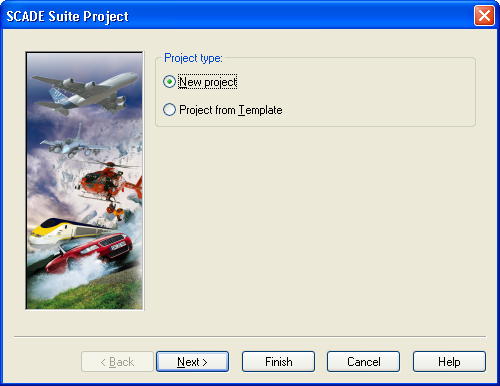
\includegraphics[width=0.55\textwidth]{imgs/scade1}
\caption{Create a new SCADE project}
\label{scade1}
\end{figure}
\begin{figure}
\centering
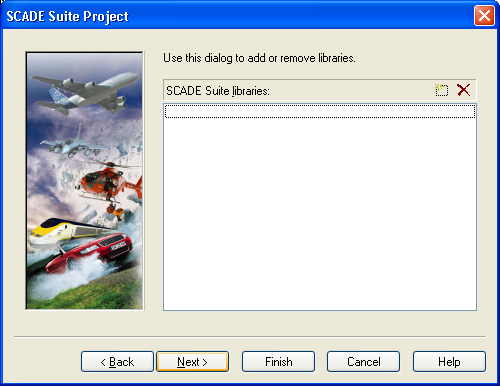
\includegraphics[width=0.55\textwidth]{imgs/scade2}
\caption{Remove default libraries}
\label{scade2}
\end{figure}
\begin{figure}
\centering
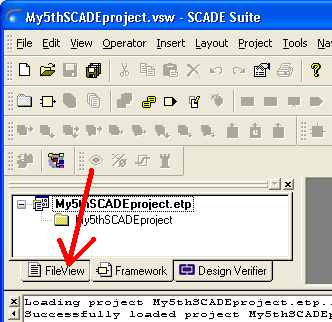
\includegraphics[width=0.45\textwidth]{imgs/scade3}
\caption{Select FileView}
\label{scade3}
\end{figure}
\begin{figure}
\centering
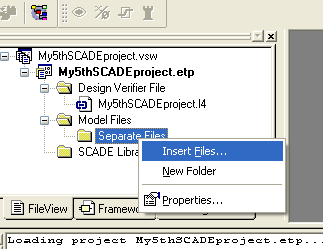
\includegraphics[width=0.45\textwidth]{imgs/scade4}
\caption{Add TASTE-generated .xscade file}
\label{scade4}
\end{figure}
\begin{figure}
\centering
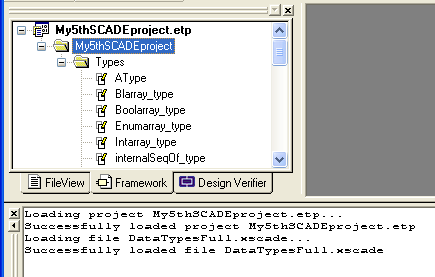
\includegraphics[width=0.5\textwidth]{imgs/scade5}
\caption{Types are now available}
\label{scade5}
\end{figure}
\begin{figure}
\centering
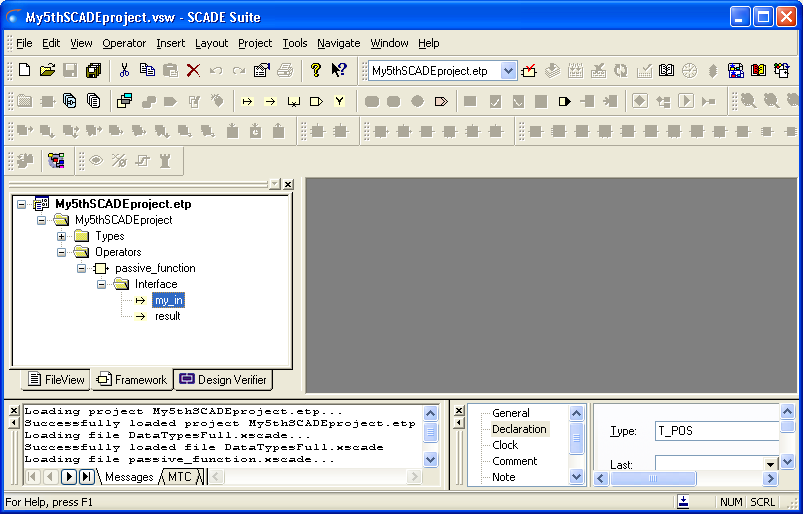
\includegraphics[width=0.95\textwidth]{imgs/scade6}
\caption{Interface skeleton generated by TASTE}
\label{scade6}
\end{figure}
\begin{figure}
\centering
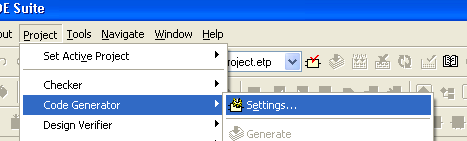
\includegraphics[width=0.55\textwidth]{imgs/scade7}
\caption{SCADE settings}
\label{scade7}
\end{figure}
\begin{figure}
\centering
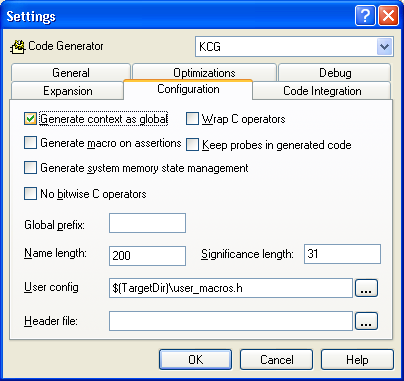
\includegraphics[width=0.55\textwidth]{imgs/scade8}
\caption{SCADE settings - Set "Global context"}
\label{scade8}
\end{figure}
\begin{figure}
\centering
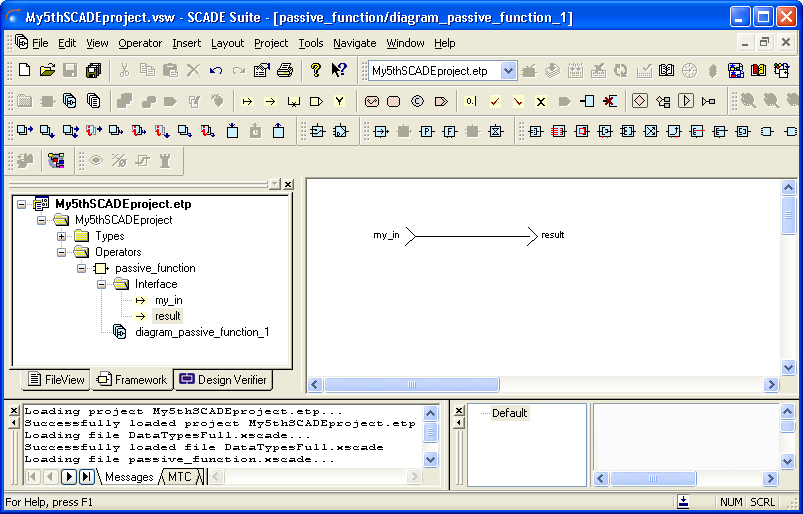
\includegraphics[width=0.95\textwidth]{imgs/scade9}
\caption{The simplest of systems - a pass-through}
\label{scade9}
\end{figure}

This allows the user to use the ASN.1 types in his SCADE Function. However, TASTE offers more than this -
it creates the SCADE "skeleton", with the parameters of the Function's interface already filled in:

\begin{lstlisting}[language=bash]
bash$ buildsupport -gw -glue -i interfaceview.aadl -c deploymentview.aadl -d DataTypesFull.aadl
...
bash$ ls -l
total 88
drwx------ 2 assert assert    80 May 17 14:38 Backdoor
drwx------ 2 assert assert   200 May 17 14:38 ConcurrencyView
-rw-r--r-- 1 assert assert 22393 May 17 14:35 DataTypesFull.aadl
-rw-r--r-- 1 assert assert  2182 May 17 14:20 DataTypesFull.asn
-rw-r--r-- 1 assert assert 46321 May 17 14:23 DataTypesFull.xscade
-rw-r--r-- 1 assert assert   126 May 17 14:38 build-sample.sh
drwx------ 2 assert assert   312 May 17 14:38 cyclic_function
-rw-r--r-- 1 assert assert  1018 May 17 14:37 deploymentview.aadl
-rw-r--r-- 1 assert assert  2242 May 17 14:37 interfaceview.aadl
drwx------ 2 assert assert   216 May 17 14:38 passive_function

bash$ cd passive_function
bash$ ls -l
total 16
-rw-r--r-- 1 assert assert  368 May 17 14:38 mini_cv.aadl
-rw-r--r-- 1 assert assert  740 May 17 14:38 passive_function.xscade
-rw-r--r-- 1 assert assert 2302 May 17 14:38 passive_function_wrappers.adb
-rw-r--r-- 1 assert assert  873 May 17 14:38 passive_function_wrappers.ads
\end{lstlisting}

Another .xscade file is generated - containing the skeleton for the SCADE Operator {\tt passive\_function}. 
By importing this file as well (as before, from the FileView, right-click/insert files), the project skeleton
is now available - see \ref{scade6}.

In order to be able to use the KCG (SCADE's code generator) output from TASTE, the user must select "Global context"
in the KCG options - see \ref{scade7} and \ref{scade8}.

After this, we can fill-in the skeleton - for example, we can create the simplest of systems (since both input and 
output are of the same type, {\tt T\_POS}): a pass-through (\ref{scade9}).

Invoking KCG, will generate our code - which we place inside a .zip file, that must contain a directory with the same
name as our SCADE Function ({\tt passive\_function}):

\begin{lstlisting}[language=bash]
bash$ mkdir package
bash$ cd package
bash$ mkdir passive_function
bash$ cp -a /path/to/kcg/generated/files/* passive_function/
bash$ zip -9 -r passive_function.zip passive_function/
\end{lstlisting}

This .zip file is the one that must be passed to the orchestrator, when using a SCADE subsystem:

\begin{lstlisting}[language=bash]
bash$ "$DMT/OG/assert-builder-ocarina.py" \
        -f \
        -o binary.linux \
        -a ./DataView.asn \
        -i ./InterfaceView.aadl \
        -c ./DeploymentView.aadl \
	...
        -S passive_function:/path/to/passive_function.zip
\end{lstlisting}

   \section{Simulink-specific}
   If a Function is coded in Simulink, then the TASTE editor must be used to
   properly select the Function's "language" field, as depicted in Figure \ref{ellidiss1}.
\begin{figure}
\centering
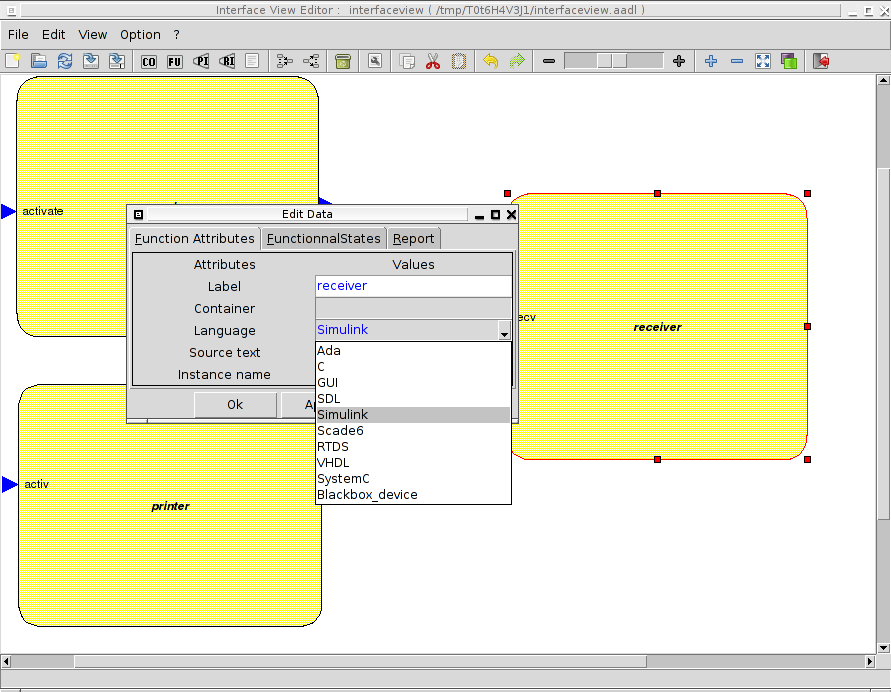
\includegraphics[width=0.85\textwidth]{imgs/iv_simulink}
\caption{Creating a Simulink/RTW function}
\label{ellidiss1}
\end{figure}
   The corresponding AADL part of the Interface View will then contain something like this:
\begin{lstlisting}[language=aadl]
  SYSTEM passive_function
  FEATURES
    compute : IN EVENT PORT
      {
        Compute_Entrypoint => "compute";
        Assert_Properties::RCMoperation => SUBPROGRAM myLib::compute;
        Assert_Properties::RCMoperationKind => unprotected;
      };
  END passive_function;
  
  SYSTEM IMPLEMENTATION passive_function.others
    PROPERTIES
      Source_Language => Simulink;
  END passive_function.others;
...
  SUBPROGRAM compute
    FEATURES
      my_in: in PARAMETER DataView::T_POS
        { Assert_Properties::encoding => UPER;};
      result: out PARAMETER DataView::T_POS
        { Assert_Properties::encoding => NATIVE;};
    PROPERTIES
      Compute_Execution_Time => 1ms..1ms;
  END compute;
\end{lstlisting}
 
In this example, a Function called {\tt passive\_function} contains a provided interface
called {\tt compute}. This interface has one input parameter and one output parameter,
which, in this example, are both of type {\tt T\_POS}. This type is described in the 
ASN.1 grammar:

\begin{lstlisting}[language=aadl]
...
T-POS ::= CHOICE {
    longitude	REAL(-180.0..180.0),
    latitude	REAL(-90.0..90.0),
    height	REAL(30000.0..45000.0),
    subTypeArray SEQUENCE (SIZE(10..15)) OF TypeNested,
    label	OCTET STRING (SIZE(50)),
    intArray	T-ARR,
...    
}

TypeNested ::= SEQUENCE {
...
}

T-ARR ::= SEQUENCE (SIZE (5..6)) OF INTEGER (0..32767)

\end{lstlisting}

This type is a complex one, referencing other types, and containing arrays ({\tt SEQUENCE OFs}), too.
Let's see how these two inputs - the ASN.1 grammar and the Interface view, are combined during TASTE development.

Invoking {\tt asn2dataModel.py} on the ASN.1 grammar:

\begin{lstlisting}[language=bash]
bash$ cd SimulinkExample
bash$ ls -l
total 12
drwxr-xr-x  2 assert assert 4096 Sep 20 10:47 ./
drwxr-xr-x 17 assert assert 4096 Sep 20 10:47 ../
-rw-r--r--  1 assert assert  903 Sep 20 10:47 DataView.asn

bash$ asn2dataModel.py -toSIMULINK DataView.asn
bash$ ls -l
total 24
drwxr-xr-x  2 assert assert 4096 Sep 20 10:48 ./
drwxrwxrwt 17 assert assert 4096 Sep 20 10:47 ../
-rw-r--r--  1 assert assert  903 Sep 20 10:47 DataView.asn
-rw-r--r--  1 assert assert 9072 Sep 20 10:48 Simulink_DataView_asn.m
\end{lstlisting}

The model mapper generates a .m file - and this file is directly importable in Matlab/Simulink.

The next steps show how:
\begin{enumerate}
\item The generated file is placed under a new directory visible from MATLAB (see \ref{matlab1})
\item Right-click on the file and selecting "Run" (see \ref{matlab2})
\item Matlab will be "Busy" while processing the type declarations (see \ref{matlab3})
\item When processing is finished, the "buseditor" command is given (see \ref{matlab4})
\item The ASN.1 types are now visible (and available to create designs) in Matlab/Simulink (see \ref{matlab5})
\end{enumerate}

\begin{figure}
\centering
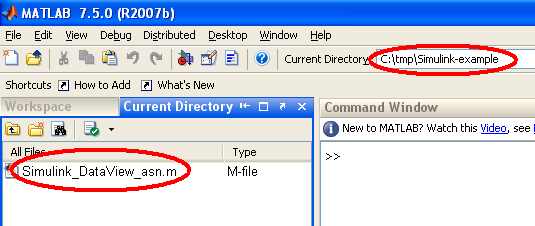
\includegraphics[width=0.55\textwidth]{imgs/matlab1}
\caption{Use the generated file under Matlab}
\label{matlab1}
\end{figure}
\begin{figure}
\centering
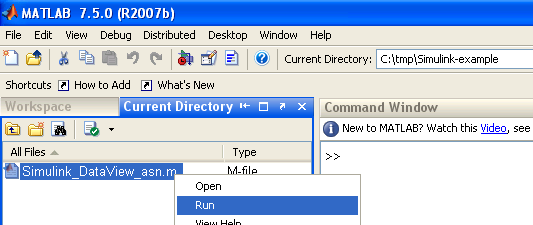
\includegraphics[width=0.55\textwidth]{imgs/matlab2}
\caption{Run the file - Matlab learns the new types}
\label{matlab2}
\end{figure}
\begin{figure}
\centering
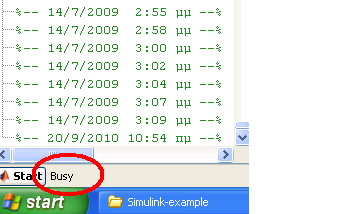
\includegraphics[width=0.45\textwidth]{imgs/matlab3}
\caption{Matlab processing (reports "Busy")}
\label{matlab3}
\end{figure}
\begin{figure}
\centering
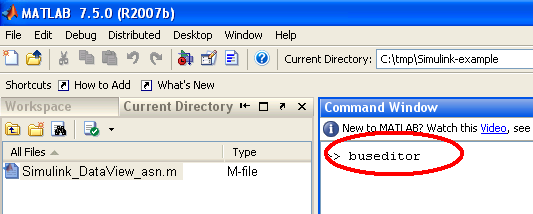
\includegraphics[width=0.45\textwidth]{imgs/matlab4}
\caption{Invoking the buseditor}
\label{matlab4}
\end{figure}
\begin{figure}
\centering
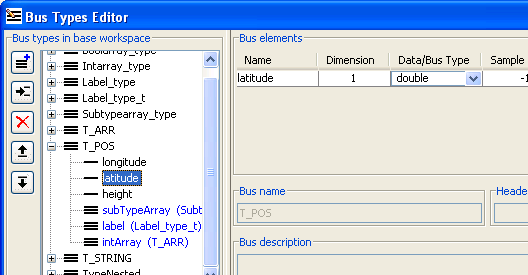
\includegraphics[width=0.5\textwidth]{imgs/matlab5}
\caption{Types are now available}
\label{matlab5}
\end{figure}
\begin{figure}
\centering
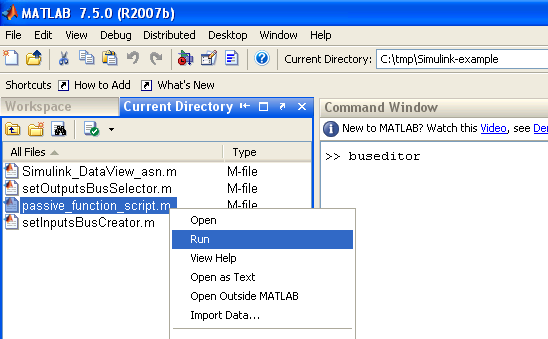
\includegraphics[width=0.95\textwidth]{imgs/matlab6}
\caption{Right-click on FUNCTIONNAME\_script.m, select Run}
\label{matlab6}
\end{figure}
\begin{figure}
\centering
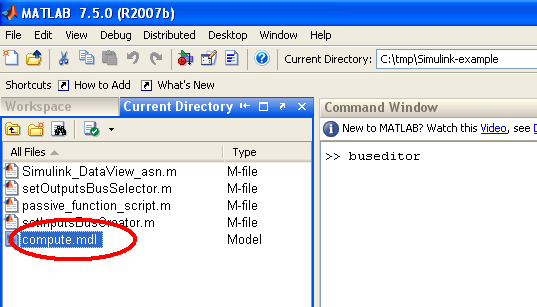
\includegraphics[width=0.55\textwidth]{imgs/matlab7}
\caption{The FUNCTIONNAME.mdl file is generated}
\label{matlab7}
\end{figure}
\begin{figure}
\centering
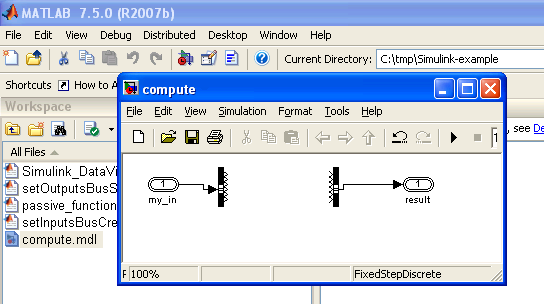
\includegraphics[width=0.55\textwidth]{imgs/matlab8}
\caption{Double-click on FUNCTIONNAME.mdl, function skeleton is shown}
\label{matlab8}
\end{figure}
\begin{figure}
\centering
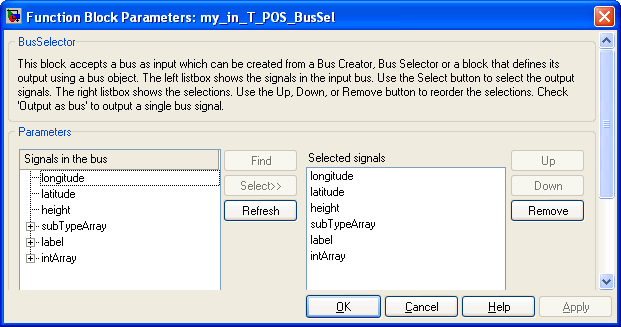
\includegraphics[width=0.95\textwidth]{imgs/matlab9}
\caption{Double-click on the my\_in bus selector, the fields are available}
\label{matlab9}
\end{figure}

This allows the user to use the ASN.1 types in his Matlab/Simulink Function. However, TASTE offers more than this -
it creates the Simulink "skeleton", with the parameters of the Function's interface already filled in:

\begin{lstlisting}[language=bash]
bash$ asn2aadlPlus.py DataView.asn DataView.aadl
bash$ buildsupport -gw -glue -i interfaceview.aadl -c deploymentview.aadl -d DataView.aadl
...
bash$ ls -lF
total 48
drwx------ 2 assert assert 4096 Sep 20 11:33 ConcurrencyView/
-rw-r--r-- 1 assert assert 9877 Sep 20 11:33 DataView.aadl
-rw-r--r-- 1 assert assert  903 Sep 20 10:47 DataView.asn
-rw-r--r-- 1 assert assert 9072 Sep 20 11:25 Simulink_DataView_asn.m
drwx------ 2 assert assert 4096 Sep 20 11:33 cyclic_function/
-rw-r--r-- 1 assert assert 1038 Sep 20 11:15 deploymentview.aadl
-rw-r--r-- 1 assert assert 2241 Sep 20 11:32 interfaceview.aadl
drwx------ 2 assert assert 4096 Sep 20 11:33 passive_function/
bash$ cd passive_function
bash$ ls -l
total 24
-rw-r--r-- 1 assert assert  371 Sep 20 11:18 mini_cv.aadl
-rw-r--r-- 1 assert assert 3901 Sep 20 11:18 passive_function_script.m
-rw-r--r-- 1 assert assert 2363 Sep 20 11:18 passive_function_wrappers.adb
-rw-r--r-- 1 assert assert  873 Sep 20 11:18 passive_function_wrappers.ads
-rw-r--r-- 1 assert assert  379 Sep 20 11:18 setInputsBusCreator.m
-rw-r--r-- 1 assert assert  291 Sep 20 11:18 setOutputsBusSelector.m
\end{lstlisting}

A set of .m files is generated - containing the skeleton for the Simulink {\tt passive\_function}. 
Placing these .m files under Simulink and executing {\em "passive\_function\_script.m"} creates the
function skeleton (\ref{matlab6}, that is the FUNCTIONNAME.mdl file. 

By double-clicking on the .mdl file, the skeleton is shown - see \ref{matlab7}, \ref{matlab8}.

Finally, by double-clicking on the bus selector of the input variable, all the message fields are shown to be available (\ref{matlab9}).

%In order to be able to use the KCG (SCADE's code generator) output from TASTE, the user must select "Global context"
%in the KCG options - see \ref{scade7} and \ref{scade8}.
%
%After this, we can fill-in the skeleton - for example, we can create the simplest of systems (since both input and 
%output are of the same type, {\tt T\_POS}): a pass-through (\ref{scade9}).
%
%Invoking KCG, will generate our code - which we place inside a .zip file, that must contain a directory with the same
%name as our SCADE Function ({\tt passive\_function}):
%
%\begin{lstlisting}[language=bash]
%bash$ mkdir package
%bash$ cd package
%bash$ mkdir passive_function
%bash$ cp -a /path/to/kcg/generated/files/* passive_function/
%bash$ zip -9 -r passive_function.zip passive_function/
%\end{lstlisting}
%
%This .zip file is the one that must be passed to the orchestrator, when using a SCADE subsystem:
%
%\begin{lstlisting}[language=bash]
%bash$ "$DMT/OG/assert-builder-ocarina.py" \
%        -f \
%        -o binary.linux \
%        -a ./DataView.asn \
%        -i ./InterfaceView.aadl \
%        -c ./DeploymentView.aadl \
%	...
%        -S passive_function:/path/to/passive_function.zip
%\end{lstlisting}
%
   \section{RTDS-specific}
   \subsection{Step 1: specify RTDS as implementation language}
   You can use RTDS to write the functional code of your system. By using RTDS,
   you design system behavior. Then, TASTE use the code generated by RTDS and
   integrates it within the architecture code, connecting all functions
   (potentially written using different languages) altogether.

   First of all, the user has to specify \texttt{RTDS} as the implementation
   language to be designed. Specification of functions implementation language
   is defined in the interface view, so, you have to add this requirement in the
   interface view (see picture below).


   \centerline{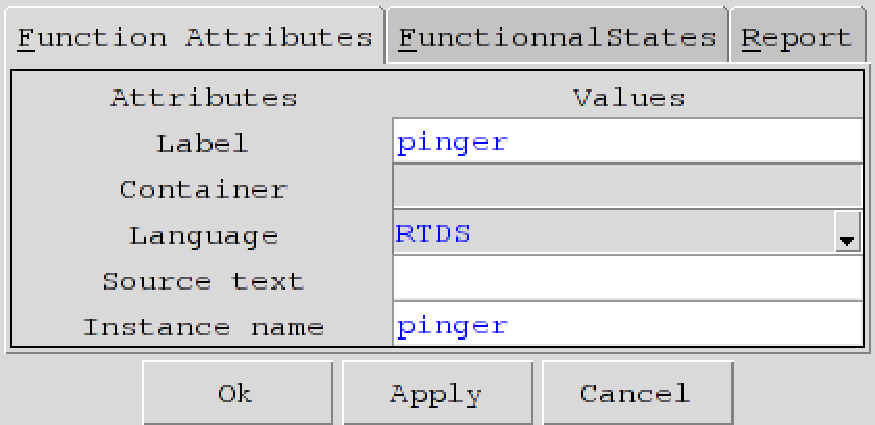
\epsfig{file=imgs/rtds-tasteiv.pdf,width=.58\textwidth}}

   \subsection{Step 2: Generate application skeletons}

   Then, once you defined your \textit{Interface view} and your \textit{Data
   view}, you can generate SDL application skeletons using
   \texttt{taste-generate-skeletons}. In this way, you'll have a new RTDS project that will
   contain signals and data types to interact with the system environment.

   To generate SDL skeletons, issue the following commands:

   \begin{verbatim}
taste-generate-skeletons InterfaceView.aadl [output_directory]
   \end{verbatim}

   \subsection{Step 3: Edit application skeletons}

   After running these commands, you have a new directory \texttt{rtds\_model}
   that contains a new RTDS project. You can open this project and define this
   subsystem behaviour using SDL:

   \begin{verbatim}
cd <rtds_model>
rtds <rtds_model>_project.rdp &
   \end{verbatim}

   The project contains a unique SDL process that represents the function. 
   \textit{Provided} and \textit{Required Interfaces} are
   specified in SDL using signals so that you can use them to communicate with
   the other entities of the TASTE systems. Synchronous interfaces are also
   available using SDL \textit{external procedures}. Finally, to ensure data consistency,
   ASN.1 data types are also embedded in your SDL project so that you can use it
   in the description of application concerns and for communication with the
   other entities of the system.

   When you run RTDS, a project like the following will be opened. Note that this project
   contains two partitions: one with the declarative part (data types import,
   etc.), another with the architecture (SDL processes, etc.).

   \centerline{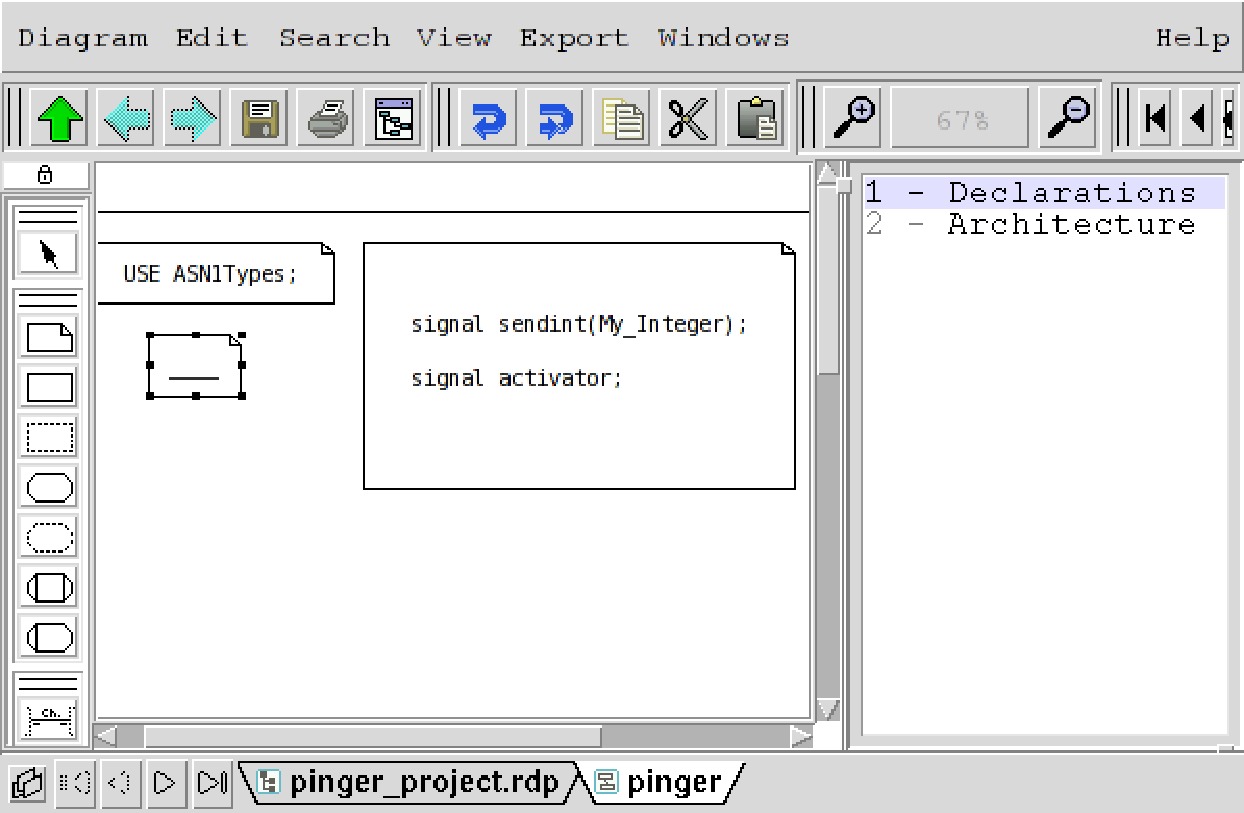
\epsfig{file=imgs/rtds-rtds.pdf,width=.98\textwidth}}

   There are a few restrictions to what you are allowed to do: (1) you must not add
   other processes or blocks to the system ; (2) internal procedures and macros are not
   supported by the RTDS code generator at the moment: do not use them ; (3) do not change
   the generated datatypes file: if you need to add new types, create an additional component
   for that purpose.

   \subsection{Step 4: Generate SDL-related code}

   Once you have edited your SDL model, close RTDS. Then, you need to generate
   the code that corresponds to this application model. This is straightforward: 

   \begin{verbatim}
./rtds_GenerateCodeForTASTE.sh
   \end{verbatim}

   If your model is correct, then you will see no error and a zip file will be created
   for you in the current directory.

   \subsection{Updating the RTDS model following a change in the interface view}
   If you modify the interface view of your system (thus go through step 2 again),
   the RTDS project file will be updated with the new interfaces. The implementation
   of your SDL process will be kept (it is saved in a separate file), however since the
   project file will be updated, you will need to re-attach the process to the project.
   
   In practice what you have to do is simple: (1) open the RTDS project (as in step 3),
   then double click on the system (to open the system architecture diagram), and then
   (2) double click on the process. The tool will ask you to choose a file to implement the
   process. Finally (3) select your (existing) file, and save everything. 


   \subsection{Use RTDS within TASTEGUI}
   To ease system development, we provide a graphical interface that
   automatically calls all TASTE components (data view generator, orchestrator,
   etc.): TASTEGUI.

   This tool is also capable to be interfaced with RTDS. When a function uses
   the RTDS implementation language, its edition automatically laucnhes RTDS. In
   addition, it produces all required files to generated RTDS/SDL-related code
   so that you don't have to worry about archive production.

   However, to be able to use RTDS within TASTEGUI, you have to specify the
   \texttt{RTDS\_HOME} environment variable, that is also required by the RTDS
   toolsuite. Be sure this variable is set in your environment before starting
   RTDS.



   \section{C- and Ada- specific}
   For these two languages, the user writes manually the code for his Function's interfaces.
   TASTE helps, by automatically generating the C/Ada header/implementation files (i.e.
   the {\tt .h/.c} files for C, or the {\tt .ads/.adb} files for Ada). 

   Here's an example, taken from the {\tt Demo\_2Cfunctions} part of the TASTE examples 
   (in the VM, check the {\tt work/testSuites} directory).

\begin{lstlisting}[language=bash]
bash$ cat DataView.asn
DataView DEFINITIONS AUTOMATIC TAGS ::= BEGIN

T-INTEGER ::= INTEGER (0..255)

END

bash$ cat interfaceview.aadl
...
SYSTEM passive_function
FEATURES
  compute : IN EVENT PORT
    {
      Compute_Entrypoint => "compute";
      Assert_Properties::RCMoperation => SUBPROGRAM myLib::compute;
      Assert_Properties::RCMoperationKind => unprotected;
    };
END passive_function;

SYSTEM IMPLEMENTATION passive_function.others
  PROPERTIES
    Source_Language => C;
END passive_function.others;
...
  SUBPROGRAM compute
    FEATURES
      my_in: in PARAMETER DataView::T_SEQUENCE
        { Assert_Properties::encoding => UPER;};
      result: out PARAMETER DataView::T_INTEGER
        { Assert_Properties::encoding => NATIVE;};
    PROPERTIES
      Compute_Execution_Time => 1ms..1ms;
  END compute;
...
\end{lstlisting}

By using the TASTE views in ESA's buildsupport, automatic skeleton projects are written for our {\tt passive\_function}:


\begin{lstlisting}[language=bash]
bash$ ls -l
total 20
drwxr-xr-x  2 assert assert 4096 Jul 28 12:58 ./
drwxr-xr-x 17 assert assert 4096 Jul 28 12:56 ../
-rw-r--r--  1 assert assert  776 Jul 28 12:56 DataView.asn
-rw-r--r--  1 assert assert 1018 Jul 28 12:56 deploymentview.aadl
-rw-r--r--  1 assert assert 2246 Jul 28 12:56 interfaceview.aadl

bash$ asn2aadlPlus.py DataView.asn DataView.aadl
bash$ ls -l
total 24
drwxr-xr-x  2 assert assert 4096 Jul 28 12:58 ./
drwxr-xr-x 17 assert assert 4096 Jul 28 12:56 ../
-rw-r--r--  1 assert assert 2571 Jul 28 12:56 DataView.aadl
-rw-r--r--  1 assert assert  776 Jul 28 12:56 DataView.asn
-rw-r--r--  1 assert assert 1018 Jul 28 12:56 deploymentview.aadl
-rw-r--r--  1 assert assert 2246 Jul 28 12:56 interfaceview.aadl

bash$ buildsupport -gw -i interfaceview.aadl  -c deploymentview.aadl -d DataView.aadl
bash$ ls -l
total 24
-rw-r--r-- 1 assert assert 2751 Jul 28 12:59 DataView.aadl
-rw-r--r-- 1 assert assert  776 Jul 28 12:56 DataView.asn
...
drwx------ 2 assert assert 4096 Jul 28 13:00 passive_function

bash$ ls -l passive_function
total 8
-rw-r--r-- 1 assert assert 382 Jul 28 13:00 passive_function.c
-rw-r--r-- 1 assert assert 372 Jul 28 13:00 passive_function.h

\end{lstlisting}

As you can see in the above example, buildsupport generated the Function's skeleton,
which includes all the necessary type and interface information:

\begin{lstlisting}[language=C]
/* This file was generated automatically: DO NOT MODIFY IT ! */

/* Declaration of the functions that have to be provided by the user */

#ifndef __USER_CODE_H_passive_function__
#define __USER_CODE_H_passive_function__

#include "C_ASN1_Types.h"

void passive_function_startup();
void passive_function_PI_compute(const asn1SccT_SEQUENCE *, asn1SccT_INTEGER *);

#endif
\end{lstlisting}

\begin{lstlisting}[language=C]
/* Functions to be filled by the user (never overwritten by buildsupport tool) */

#include "passive_function.h"

void passive_function_startup()
{
        /* Write your initialization code here,
           but do not make any call to a required interface!! */
}

void passive_function_PI_compute(const asn1SccT_SEQUENCE *IN_my_in, asn1SccT_INTEGER *OUT_result)
{
        /* Write your code here! */
}
\end{lstlisting}

Very similar things happen for Ada Functions, where the generated files are the corresponding .ads/.adb:

\begin{lstlisting}[language=Ada]
-- This file was generated automatically: DO NOT MODIFY IT !

-- Declaration of the provided and required interfaces

pragma style_checks (off);
pragma warnings (off);
with adaasn1rtl;
use adaasn1rtl;

with dataview;
use dataview;

package passive_function is

        ---------------------------------------------------------
        -- Provided interface "compute"
        ---------------------------------------------------------
        procedure compute(my_in: access asn1sccT_SEQUENCE; result: access asn1sccT_INTEGER);
        pragma export(C, compute, "passive_function_PI_compute");


end passive_function;
\end{lstlisting}

\begin{lstlisting}[language=Ada]
-- User implementation of the passive_function function
-- This file will never be overwritten once edited and modified
-- Only the interface of functions is regenerated (in the .ads file)

pragma style_checks (off);
pragma warnings (off);
with adaasn1rtl;
use adaasn1rtl;

with dataview;
use dataview;

package body passive_function is

        ---------------------------------------------------------
        -- Provided interface "compute"
        ---------------------------------------------------------
        procedure compute(my_in: access asn1sccT_SEQUENCE; result: access asn1sccT_INTEGER) is
        begin

                null; -- Replace "null" with your own code!

        end compute;


end passive_function;
\end{lstlisting}

After filling-in the code, the user must simply zip the contents in the directories:

\begin{lstlisting}[language=bash]
bash$ mkdir package
bash$ cd package
bash$ mkdir passive_function
bash$ cp -a /path/to/user-filled/files/passive_function.[ch] passive_function/
bash$ zip -9 -r passive_function.zip passive_function/
\end{lstlisting}

This .zip file is the one that must be passed to the orchestrator:

\begin{lstlisting}[language=bash]
bash$ "$DMT/OG/assert-builder-ocarina.py" \
        -f \
        -o binary.linux \
        -a ./DataView.asn \
        -i ./InterfaceView.aadl \
        -c ./DeploymentView.aadl \
	...
        -C passive_function:/path/to/passive_function.zip
\end{lstlisting}

TASTE therefore completely automates the interface specification, allowing the user
to focus on the implementation logic of his interfaces. The passing of the parameters
via PolyORB, the encodings/decodings via ASN.1, endianess issues, etc, are all
handled via TASTE.

\chapter{Use \aadl models without graphical tools}
You can also write the AADL views of a TASTE system by hand. In that case,
you will need to write \aadl models and ASN.1 types definitions by yourself. 
The \textbf{Interface View} and \textbf{Deployment View} are \aadl models while
the \textbf{Data View} includes the ASN.1 data types' definitions. We don't explain how to
write the \textbf{Data View}: there are many tutorials about ASN.1 and we don't
use exotic features of this language - only the basics (type declarations and 
constraints). On the contrary, we use special \aadl
constructs for the \textbf{Interface View} and the \textbf{Deployment View} so
we detail below the modeling patterns for each view.

   \section{Writing your Interface View manually}

      \subsection{Main system of an interface view}
      The main system implementation of a \taste functional view is contained in
      a default package called \texttt{default::IV}. This system  is called by
      default \texttt{SYSTEM IMPLEMENTATION default.others} and contains
      \texttt{system} subcomponents, each one representing a function. This
      \texttt{system} component also connects each function according to their
      required/provided interfaces.

      The default package that contains the main system defines the location of
      the \textit{data view}. It is specified using the properties
      \texttt{TASTE::dataView} and \texttt{TASTE::dataViewPath}. The value of
      the \texttt{TASTE::dataView} property should be the string
      \textit{"DataView"} and the property \texttt{TASTE::dataViewPath} should
      specify the location (file) that contains the AADL data view file.


      \subsection{Model a container}
      A container is specified using an \aadl \texttt{package}. By default, the
      interface view editor creates package named like this: \texttt{PACKAGE
      default::IV::CONTAINERNAME}, where \texttt{CONTAINERNAME} is the name of
      your container.

      This package contain \texttt{system} components, each one represent a
      function.

      \subsection{Model a function}
      A function is represented by a \texttt{system} component. The property
      \texttt{Source\_Language} represents the implementation language of the
      function (C, Ada, Simulink, etc.).
      For each provided or required interface, we add a feature in the
      \texttt{system} specification.
      
      
      For example, the following component models
      a function that provides a single interface. The function is implemented
      using the C language.

      \begin{lstlisting}[language=aadl]
  SYSTEM function2
    FEATURES
      provided1 : PROVIDES SUBPROGRAM ACCESS default::FV::provided1
      {
         --  provided interfaces properties.
      };
    PROPERTIES
      Source_Language => C;
      Taste::Coordinates => "91 27 109 50";
  END function2;
      \end{lstlisting}

 
      The following component models
      a function that requires a single interface. The function is implemented
      using the Ada language.

      \begin{lstlisting}[language=aadl]
  SYSTEM function1
    FEATURES
      required1 : REQUIRES SUBPROGRAM ACCESS default::FV::bla
        { 
        --  required interface properties.
        };
    PROPERTIES
      Source_Language => Ada;
      Taste::Coordinates => "14 14 35 45";
  END function1;
      \end{lstlisting}

      \subsection{Model a provided interface}
      A provided interface is represented using two \aadl artifacts:
      \begin{enumerate}
         \item
            A subprogram component. 
         \item
            A \texttt{provides subprogram access} feature in the \aadl \texttt{system} component that represents the
            function containing this provided interface.
      \end{enumerate}

      The \texttt{subprogram} component has the same name as the provided
      interface name. By default, the interface view editor adds all subprogram
      components in a default package called \texttt{default::FV}.

      \texttt{Subprogram} components declare features for their parameters.
      These parameters use the types from the Data View. For example, the
      following component (\texttt{provided1}) declares a \texttt{subprogram}
      component for a provided interface called \texttt{provided1} having one
      parameter one type \texttt{TM\_T}.
      \begin{lstlisting}[language=aadl]
  SUBPROGRAM provided1
    FEATURES
      paramin1 : in PARAMETER DataView::TM_T
        { Taste::encoding => NATIVE; };
  END provided1;
      \end{lstlisting}


      The feature added in the \texttt{system} that represents the function
      which contains the interface specifies all the properties of the
      interface (type, importance, etc.). For example, the following
      \texttt{system} component (\texttt{function2}) provides an access to the
      interface \texttt{provided1}. 

      \begin{lstlisting}[language=aadl]
  SUBPROGRAM provided1
  SYSTEM function2
    FEATURES
      provided1 : PROVIDES SUBPROGRAM ACCESS default::FV::provided1
      {
        Taste::RCMoperationKind => sporadic;
        Taste::RCMperiod => 0 ms;
        TASTE::Compute_Execution_Time => 0 ms .. 100ms;
        Taste::Deadline => 0 ms;
        Taste::Importance => MEDIUM ;
        Taste::Coordinates => "89 45 91 47";
      };
    PROPERTIES
      Source_Language => C;
      Taste::Coordinates => "91 27 109 50";
  END function2;
  \end{lstlisting}
   Here, the following properties are added to the provided interface:
   \begin{enumerate}
      \item
         \texttt{Taste::RCMoperationKind}: indicates the kind of the interface.
         The value can be sporadic, periodic, protected or unprotected. This
         property is defined in the Taste-specific property set.
      \item
         \texttt{Taste::RCMPeriod}: specifies the period at which the interface
         can be called. This property is defined in the Taste-specific property
         set.
      \item
         \texttt{Taste::Importance}: specifies if an interface is more important
         (in terms of priority) than another. The value can be low, medium or
         high.
      \item
         \texttt{Compute\_Execution\_Time}: specifies the execution time of the
         code. The value is a time range. This property is defined in the
         standard \aadl property set.
      \item
         \texttt{Taste::Deadline}: specifies when the job associated with the interface
         should be completed. This property is defined in Taste-specific
         property set.
   \end{enumerate}

      \subsection{Model a required interface}
      A provided interface is represented by a
      \texttt{requires subprogram access} feature in the \aadl \texttt{system} 
      component (\taste function) that calls the interface.

      The required \texttt{subprogram} component is defined in the
      \texttt{default::FV} package. It was defined when the user write the
      provided subprogram for this interface (see previous section).

      The feature added in the \texttt{system} that represents the function
      that calls this interface specifies all the properties of the
      interface (type, importance, etc.). For example, the following
      \texttt{system} component (\texttt{function1}) provides an access to the
      interface \texttt{provided1}. 

      \begin{lstlisting}[language=aadl]
  SYSTEM function1
    FEATURES
      required1 : REQUIRES SUBPROGRAM ACCESS default::FV::bla
        { Taste::Coordinates => "35 41 37 43"; };
    PROPERTIES
      Source_Language => C;
      Taste::Coordinates => "14 14 35 45";
  END function1;
      \end{lstlisting}

      We don't need to specify additional properties since all required
      properties are declared in the declarations of the provided interface. 


      \subsection{Connect provided and required interfaces}
      The interface view contains a single system that gathers all functions or
      your system. By default, the interface view editor creates a system
      implementation called \texttt{default.others}, which contains all
      functions (\texttt{system} components) and connects their features.

      By connecting their features, it associates provided and required
      interface.

      In the following example, the system \texttt{default.others} contains 4
      functions. It connects function1 and function2: the interface provided by
      \texttt{function2} (\texttt{provided1}) is connected to the interface
      required by \texttt{function1} (\texttt{required1}).

      \begin{lstlisting}[language=aadl]
  SYSTEM default
  END default;

  SYSTEM IMPLEMENTATION default.others
    SUBCOMPONENTS
      function1: SYSTEM default::IV::container::function1.others
        { Taste::Coordinates => "14 14 35 45"; };
      function2: SYSTEM default::IV::container::function2.others
        { Taste::Coordinates => "91 27 109 50"; };
      function3: SYSTEM default::IV::container2::function3.others
        { Taste::Coordinates => "135 33 155 70"; };
      function4: SYSTEM default::IV::container2::function4.others
        { Taste::Coordinates => "135 73 185 94"; };
    CONNECTIONS
      conn1 : SUBPROGRAM ACCESS function2.provided1  -> function1.required1 
        { Taste::Coordinates => "35 42 63 42 63 46 91 46"; };
  END default.others;
      \end{lstlisting}

      \subsection{About AADL properties of the interface view}
      The \texttt{TASTE::Coordinates} property was introduced to describe where
      components are located in the graphical example. If you are using only
      textual representation, they can be ommitted.

      The list of all \taste-specific \aadl properties is available in section 
      \ref{taste-aadl-properties}.

      \subsection{Example of a manually written interface view}
      The following example details the modeling of an interface view with AADL.
      We provide the graphical representation as well to help the reader to
      understand the mapping between the graphic representation and the textual
      one.

      \centerline{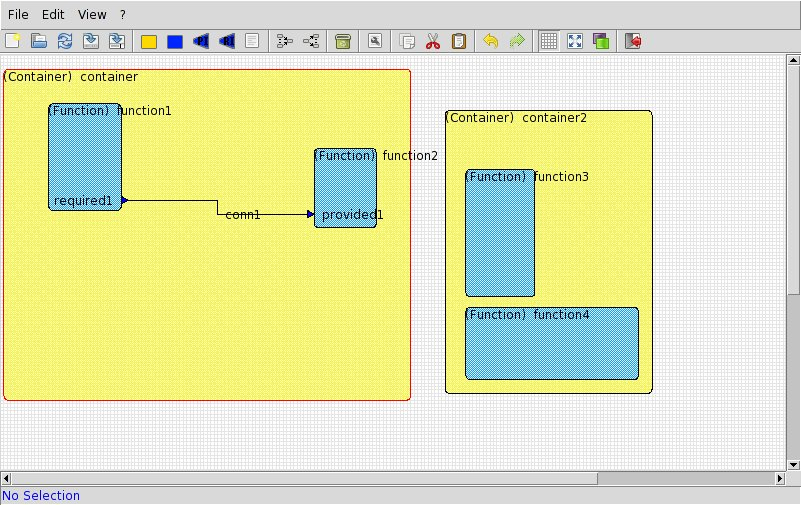
\epsfig{file=imgs/iv_example.pdf,width=.98\textwidth}}

      \lstinputlisting[language=aadl]{iv_example.aadl}

   \section{Writing your Deployment View manually}

      \subsection{Model a processor board}

      \subsection{Model a processor}

      \subsection{Model a partition}

      \subsection{Model a memory}

      \subsection{Model a device}


      \subsection{Example of a manually written deployment view}
      The following example details the modeling of a deployment view with AADL.
      We provide the graphical representation as well to help the reader to
      understand the mapping between the graphic representation and the textual
      one.

      \centerline{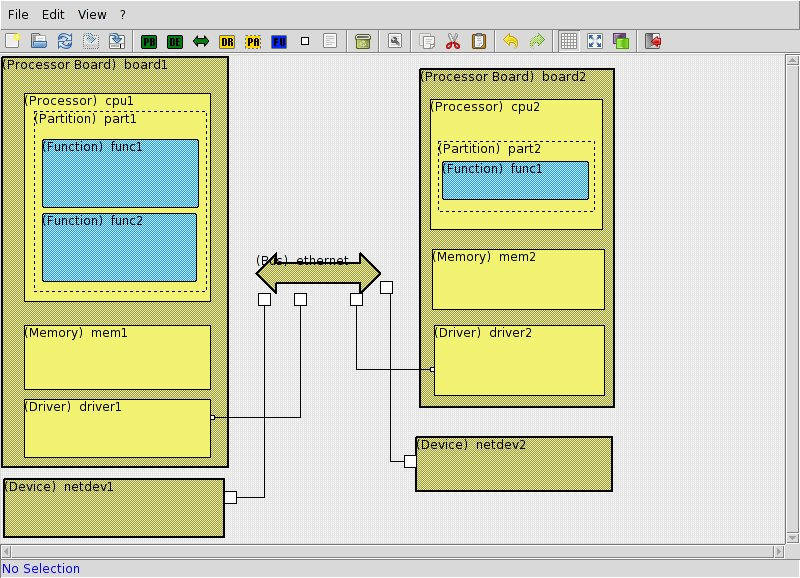
\epsfig{file=imgs/deploymentview-ex.pdf,width=.98\textwidth}}

      \lstinputlisting[language=aadl]{dv_example.aadl}


   \section{Device driver modelling}
   Devices are specified with the \aadl \texttt{device component}. These
   components model the device and the buses they use (ethernet, spacewire,
   etc.).
   
   Device drivers internals are described using \aadl properties. The
   initialization thread is specified using the
   \texttt{Initialize\_Entrypoint} on the device. The device driver resources
   are specified using an \aadl \texttt{abstract} component that is
   associated with the device using the \texttt{Device\_Driver} property on
   the device. This component describes \texttt{thread}, \texttt{data} and
   \texttt{subprogram} used for implementation purpose.

   \section{\aadl device driver library}
   Ocarina provides a set of predefined devices you can use in your models.
   This set of components can be found in the \texttt{resources/AADLv2/}
   directory of Ocarina sources, or in the
   \texttt{INSTALLDIR/share/ocarina/AADLv2} (where \texttt{INSTALLDIR} is the
   installation directory of Ocarina).

   Then, you can directly associated the device in your model, since Ocarina
   automatically integrates this component when it parses and analyzes
   models. For example, the following model add an ethernet/ip device in the
   system being configured with the IP address \texttt{192.168.0.10} and listening for
   incoming connections on port \texttt{45678}.

      \begin{lstlisting}[language=aadl]
with ocarina_devices;

system main.i
subcomponents
   netif : device ocarina_devices::eth_linux.raw
            {Deployment::Configuration => "ip 192.168.0.10 45678";}:
end main.i;
      \end{lstlisting}

      \section{Device driver configuration (the
      \texttt{Deployment::Configuration} property)}
      When you associate a device, you must configure it, it means:
      \begin{enumerate}
         \item
            Specify the type of device it implements
         \item
            Configuration items (such as IP address, device node, etc.)
      \end{enumerate}

      For that purpose, the designer binds the
      \texttt{Deployment::Configuration} property. The value of the property is clearly
      defined for each kind of device driver:
      \begin{enumerate}
         \item
            For \textbf{sockets/ip driver}, the value of the property is \texttt{ip
            ip\_addr ip\_port}. For example the value \texttt{ip 192.168.0.1 1234}
            specifies that the device is a network device with an IP stack, it
            is associated with the address 192.168.0.1 and listen for incoming
            connections on port 1234.
         \item
            For \textbf{spacewire driver}, the value of the property is
            \texttt{spacewire SENDER\_CORE\_ID RECEIVER\_CORE\_ID}. For example,
            the value \texttt{spacewire 4 5} specifies a spacewire device that
            will communicate through spacewire cores 4 and 5.
         \item
            For \textbf{serial drivers}, the value of the property is
            \texttt{serial DEVICE BAUDS  DATA\_BITS PARITY STOP\_BIT}. For
            example, the value \texttt{serial /dev/ttyS0 9600 8 N 1} specified a
            device that will use \texttt{/dev/ttyS0} at 9600 bauds. It will use
            8 bits for each caracter, use parity and one stop bit. For more
            information about serial line configuration, interested can refer to
            the following web
            article\footnote{\url{http://en.wikipedia.org/wiki/Serial\_port}}
      \end{enumerate}

\chapter{Toolset usage}

   \section{ASN.1 tools}
   ASN.1 tools are used to transform ASN.1 types definitions into AADL models
   as well as functional modelling representations (SCADE models, Simulink models,
    Ada/C code, etc).

      \subsection{Convert ASN.1 types into AADL models}
      To be able to use the ASN.1 type definitions with \aadl models (and thus, with your
      \textbf{interface} and \textbf{deployment} views), you must convert ASN.1
      type definitions into AADL models. The resulting AADL model will
      contain \texttt{data} components that represent the ASN.1 types.

      For that purpose, the tool \texttt{asn2aadlPlus} automatically converts
      ASN.1 definitions into AADL models. You can use it as it:
      \begin{lstlisting}[language=bash]
asn2aadlPlus datadefinition1.asn  ... datadefinitionX.asn outputfile.aadl
      \end{lstlisting}

      It will process all ASN.1 files given in the command line parameter list, and output an AADL
      specification that describes ASN.1 types in \texttt{outputfile.aadl}.

      If you use the version 2 of the \aadl language, you must use the switch
      \texttt{-aadlv2}. So, the command would be:

      \begin{lstlisting}[language=bash]
asn2aadlPlus -aadlv2 datadefinition1.asn  ... datadefinitionX.asn 
             outputfile.aadl
      \end{lstlisting}

      \subsection{Convert ASN.1 types into Functional Data Models}
      When building your application, you need to generate interfaces of your
      ASN.1 types with your architecture and your application. For that purpose,
      the tool \texttt{asn2dataModel} exports ASN.1 data types definitions into
      a representation that is suitable for the tools you use to develop your Functions: Ada, C,
      Simulink/RTW, SCADE/KCG, ObjectGeode or PragmaDev (Python is also supported, 
      for scripting purposes).

      The tool should be invoked like this:

      \begin{lstlisting}[language=bash]
asn2dataModel -toC datadefinition1.asn  ... datadefinitionX.asn 
      \end{lstlisting}

      It will output a file that will contain the data type definition in the
      language you selected. For example, in our example, the switch
      \texttt{-toC} indicates that we generate interfaces for the C language.
      You can replace this switch with the following:
      \begin{itemize}
         \item
            \texttt{-toAda}: generate Ada type declarations
         \item
            \texttt{-toC}: generate C type declarations
         \item
            \texttt{-toPython}: generate Python declarations
         \item
            \texttt{-toRTDS}: generate PragmaDev/RTDS declarations
         \item
            \texttt{-toSIMULINK}: generate Simulink type declarations
         \item
            \texttt{-toOG}: generate ObjectGeode type declarations
         \item
            \texttt{-toSCADE5}: generate SCADE5 type declarations
         \item
            \texttt{-toSCADE6}: generate SCADE6 type declarations
      \end{itemize}

      For example, the following command exports data types definition contained
      in the \texttt{data.asn1} file into a representation suitable for
      Simulink.

      \begin{lstlisting}[language=bash]
asn2dataModel -toSIMULINK data.asn1
      \end{lstlisting}


\section{Ocarina and PolyORB-HI}

Ocarina is used transparently through the orchestrator. This tool is
in charge of combining all models and source code bound in the
interface and deployment views. This process is sophisticated. Therefore, 
we do not support the direct use of Ocarina as part of the TASTE toolchain.

\section{TASTE daemon (\texttt{tasted})}
The TASTE daemon program (\texttt{tasted}) is a network daemon used for several
purposes:
\begin{enumerate}
   \item
      Execute programs remotely
   \item
      Ease the test and the execution of generated applications when it requires
      a dedicated setup or deployment (for example, when a program requires to
      be run with a specific emulator/simulator or monitoring program).
   \item
      Receive requests relative to the components database and handle them.
\end{enumerate}

The programs does not use special options to be executed, just invoke it as an
usual program (such as \texttt{./tasted}). However, please note that
\texttt{tastegui} automatically executes it when starting. In consequence, if
you use \texttt{tastegui}, you probably don't have to start \texttt{tasted}
manually.

However, if this program does not require any specific options for its
invocation, it needs to be configured. Configuration files and their associated
directives are described in the chapter \ref{chapter-tasted}.

Also, for users that want to execute binaries using tasted and a command-line
interface, a dedicated tool, \texttt{tasted-cli} has been designed. Its uses is
described in \ref{chapter-tasted}.

\section{TASTE database editor (\texttt{taste-db-editor.pl}) usage}
\label{label-db-editor-usage}
The program \texttt{taste-db-editor.pl} is used to edit, modify and update
the TASTE components database. It is a text-based program that performs
operations on the TASTE components database used by the other tools
(\texttt{TASTE-IV}, \texttt{TASTE-DV}, \texttt{Orchestrator}, \ldots).

The tool is invoked by specifying a command following by one or several
arguments, like this:
\begin{verbatim}
taste-db-editor.pl command arg1 arg2 arg3 ...
\end{verbatim}

Configuration files and program dependencies are detailed in sections
\ref{db-editor-requirements} and \ref{db-editor-configuration}.

There is the list of available commands classified by groups:
\begin{itemize}
   \item
      \textbf{Printing functions}
         \begin{itemize}
            \item
               \textbf{showall} - list all components, profiles, tags and files
            \item
               \textbf{showall-components} - list all components
            \item
               \textbf{showall-profiles} - list all profiles
            \item
               \textbf{showall-files} - list all files
            \item
               \textbf{showall-tags} - list all tags
            \item
               \textbf{showall-types} - list all components types
            \item
               \textbf{show-component name} - show a specific component that is
               registered under \textbf{name}
            \item
               \textbf{show-profile name}- show the profile that registered with
               \textbf{name}.
            \item
               \textbf{show-tag name} - show the tag \textbf{name}
            \item
               \textbf{show-file name} - show the file with the appropriate
               \textbf{name}
        \end{itemize}
   \item
      \textbf{Creation functions}
      \begin{itemize}
         \item
            \textbf{create-file name description type} - register a new file in
            the database. The name of the file is \textbf{name} and the second
            and third argument provide a description and specify the file type.
            \textbf{Important}: this register the file in the database but do
            not associate the file with one component and do not specify the
            content of the file:
            \begin{enumerate}
               \item
                  to fill and specify the content of the file,
                  you can use the \textbf{put-file-content} command.
               \item
                  to associate the file with a component, you can use the
                  \textbf{add-dep} command.
            \end{enumerate}
         \item
            \textbf{create-profile name description} - create a new profile with
            an appropriate description.
         \item
            \textbf{create-tag name description} - create a new tag with the
            appropriate \textbf{name} and \textbf{description}
         \item
            \textbf{create-component name type desc profile} - create a new component
            with the name \textbf{name}. This new component has the type
            \textbf{type}, the description \textbf{desc} and is associated with
            the profile \textbf{profile}. To list all existing profiles, you can
            use the \textbf{showall-profiles} command. To list all existing
            types, you can use the \textbf{showall-types} command.
      \end{itemize}
   \item
      \textbf{Delete functions}
      \begin{itemize}
         \item
            \textbf{delete-file name} - delete the file \textbf{name}.
         \item
            \textbf{delete-profile name} - delete the profile \textbf{name}
         \item
            \textbf{delete-tag name} - delete the tag \textbf{name}
         \item
            \textbf{delete-component name} - delete the component \textbf{name}
         \item
            \textbf{delete-type name} - delete a component type with \textbf{name}
      \end{itemize}

   \item
      \textbf{Association functions}
      \begin{itemize}
         \item
            \textbf{link-file cname fname} - associate the component
                                    \textbf{cname} with the file \textbf{fname}
         \item
            \textbf{unlink-file cname fname} - remove the association between
                                    the component \textbf{cname} and the file \textbf{fname}
         \item
            \textbf{link-tag cname tname} - associate the component
                                            \textbf{cname} with the tag \textbf{tname}
         \item
            \textbf{unlink-tag cname tname} - remove the association between component
                                             \textbf{cname} and the tag \textbf{tname}
         \item
            \textbf{add-dep src\_name dst\_name type} - mark component \textbf{src\_name}
                                 dependent from component \textbf{dst\_name}
                                 with the dependency type \textbf{type}. Type
                                 can have the following values:
                                 \begin{itemize}
                                    \item
                                       \texttt{collocated}: in that case,
                                       components \texttt{src\_name} has to be
                                       collocated with component
                                       \texttt{dst\_name}.
                                    \item
                                       \texttt{provides}: in that case,
                                       components \texttt{src\_name} has to be
                                       provides the functionalities of
                                       component \texttt{dst\_name}.
                                    \item
                                       \texttt{contained}: the component
                                       \texttt{src\_name} has to be located
                                       within a component \texttt{dst\_name}.
                                 \end{itemize}
         \item
            \textbf{rm-dep src\_name dst\_name} - remove the dependency between
                                    component \textbf{src\_name} and component \textbf{dst\_name}
      \end{itemize}
   \item
      \textbf{Update functions}
      \begin{itemize}
         \item
            \textbf{update-tag name desc} - Update tag name with the next description desc
         \item
            \textbf{update-type name desc} - Update the type name with the new description desc
         \item
            \textbf{update-profile name desc} - Change the description of
            profile \textbf{name} with the argument \textbf{desc}.
         \item
            \textbf{update-component-type name newtype} - change the type
            associated with the component \textbf{name} and use
            \textbf{newtype}.
         \item
            \textbf{update-component-desc name newdesc} - change the description
            of the component \textbf{name} to \textbf{newdesc}.
         \item
            \textbf{update-component-profile name newprofile} - change the
            profile of the component \textbf{name} to \textbf{newprofile}.
         \item
            \textbf{update-file-desc name newdesc} - change the description of
            the file \textbf{name} with \textbf{newdesc}.
         \item
            \textbf{update-file-type name newtype} - change the type of the file
            \textbf{name} with \textbf{newtype}.
      \end{itemize}

   \item
      \textbf{Files operations functions}
      \begin{itemize}
         \item
            \textbf{show-file-content name} - show the content of the file
            \textbf{name}.
         \item
            \textbf{put-file-content name} - define the content of the file \textbf{name} by reading
            on the standard input.
      \end{itemize}
\end{itemize}

\section{Orchestrator}
Invoking the orchestrator without parameters shows the available options:

\lstinputlisting{orchestrator.options}

The following paragraph describes each option.

\begin{itemize}

\item[-f] When this option is NOT used, the orchestrator will pause between
compilation stages, allowing the user to inspect the build process as it unfolds.

\item[-g] When this option is used, the generated binaries include debug information
and can be debugged via local or remote GDBs.

\item[-p] When this is used, the compilation is using PolyORB-HI-C instead of the default PolyORB-HI-Ada.
If all Functions are using only C code, this will cause a decrease in the generated binary size,
since Ada's run-time won't be linked-in.

\item[-r] Uses the appropriate GCC coverage options to allow invocation of gcov on the generated binary (only for Linux builds).

\item[-h] Create binaries that can be profiled with gprof

\item[-o] Specify the output directory where the generated code and binaries will be placed.

\item[-s] This option specifies how much stack size to use (in KB). This depends on your Functional code; set it appropriately.

\item[-i] This option specifies the interface view (AADL file).

\item[-c] This option specifies the deployment view (AADL file).

\item[-S] This option specifies that the "name" Function is implemented in SCADE/KCG,
        and the "zipFile" contains the SCADE/KCG generated C code for the Function.

\item[-M] This option specifies that the "name" Function is implemented in Simulink/RTW,
        and the "zipFile" contains the Simulink/RTW generated C code for the Function.

\item[-C] This option specifies that the "name" Function is implemented in manually written C code,
        and the "zipFile" contains the C code for the Function.

\item[-A] This option specifies that the "name" Function is implemented in manually written Ada code,
        and the "zipFile" contains the Ada code for the Function.

\item[-G] This option specifies that the "name" Function is implemented in ObjectGeode,
        and the .pr files that implement the Function are provided as arguments.

\item[-P] This option specifies that the "name" Function is implemented in PragmaDev/RTDS,
        and the "zipFile" contains the generated C code for the Function.

\item[-V] This option specifies that the "name" Function is implemented as a Leon/VHDL component.
        TASTE will automatically generate the driver component necessary, so no "zipFile" is used.

\item[-e] If additional C code (not Function-specific) is needed, this option specifies an extra directory 
         containing the additional .c files to be compiled and linked in, in a specific target partition 
	 (the form is: "partitionName:/path/to/src/files/"). If more than one extra directory is
         needed, then this option must be used more than one times.

\item[-d] If additional Ada code (not Function-specific) is needed, this option specifies the directory 
         containing the additional Ada files to be compiled and linked in, in a specific target partition 
	 (the form is: "partitionName:/path/to/src/files/"). If more than one extra directory is
         needed, then this option must be used more than one times.

\item[-l] If additional "black-box" libraries are neeeded during linking, this option specifies them.
          Just like "-e" and "-d", the first part of the argument is the target partition (form is:
	  deploymentPartition:/path/to/libLibrary1.a,/path/to/libLibrary2.a,...)

\end{itemize}

   \section{Real-time MSC monitoring}
If your system was designed with a GUI block configured (i.e. your AADL definition includes a \texttt{SUBPROGRAM}
with \texttt{Source\_Language => GUI}), then the TASTE build mechanisms will automatically create a Graphical
User Interface that allows you to invoke TCs and see the incoming TM values (see \ref{gui1}). 

Additionally, the TASTE tools \texttt{tracer.py} and \texttt{tracerd.py} allow a direct link of the GUIs with
the freely available PragmaDev MSC Tracer\footnote{MSC Tracer available at \url{http://www.pragmadev.com/product/tracing.html}.}.
The user first starts the MSC Tracer (see figure \ref{msc1}), and clicks on "New Trace". Then, \texttt{tracerd.py} is spawned:

      \begin{lstlisting}[language=bash]
bash$ tracerd.py <ipAddressOfMSCTracer> <portOfMSCTracer>
      \end{lstlisting}

\begin{figure}
\centering
\includegraphics[width=0.65\textwidth]{imgs/msc1}
\caption{Spawning the MSC Tracer, and starting a new trace}
\label{msc1}
\end{figure}

The IP address of the machine running the MSC Tracer and the port number of the MSC tracer (as configured in the "Options..." dialog)
must be provided to \texttt{tracerd.py}.

After that, the user must simply spawn the automatically generated TASTE GUI applications, under the supervision of \texttt{tracer.py}:

      \begin{lstlisting}[language=bash]
bash$ tracer.py <ipAddressOfTracerd.py> 27182 <filenameOfGUIBinary>
      \end{lstlisting}

The port, hardcoded as 27182, can be modified if desired by editing \texttt{tracerd.py}. The TCs and TMs sent and received will then
be monitored in real-time in the MSC tracer, as seen in \ref{mscRepeated}.

\begin{figure}
\centering
\includegraphics[width=0.5\textwidth]{imgs/msc}
\caption{Automatic monitoring of TM/TCs via MSC Tracer}
\label{mscRepeated}
\end{figure}

\subsection{Recording of TM/TCs and playback via Python scripts}

Sending the message data for real-time ploting via the MSC tracer is one option: another is for the data to be saved (i.e. recorded) into an .msc file (\ref{mscRecorded}). The generated .msc file can then be fed to {\tt msc2py}, which will convert the recorded .msc trace into a Python script. This script can then be used at a subsequence execution (i.e. at run-time) to "replay" the scenario, sending the exact same TCs, and expecting (and verifying) the incoming TM data against the recorded ones.

\begin{figure}
\centering
\includegraphics[width=0.9\textwidth]{imgs/record-msc}
\caption{Recording TM/TCs}
\label{mscRecorded}
\end{figure}

A video showing the process \footnote{Use Videolan to play the video: get it from \url{http://www.videolan.org}} (demonstrating the usage of {\tt tracerGUI.py} and {\tt msc2py}) is here: \url{http://semantix.gr/assert/Msc.flv}.

\chapter{Using SQL databases}

By using ASN.1 as the basis of all types in all subsystems, TASTE allows for automatic serialization/deserialization of any type instance inside SQL databases. The TASTE developer does not need to write any code to achieve this; any instances can be serialized to automatically created database tables, that mirror the semantic content of the ASN.1 definitions, and also express -  to the maximum possible extent\footnote{To the extent that the underlying database engine supports them, ASN.1 constraints (integer ranges, etc) are mapped to SQL constraints.} the corresponding ASN.1 constraints.

\section{Creating only the database schema}

If the TASTE user does not wish to use the full automation described in the following section, and only wishes to obtain a semantically equivalent database schema for his ASN.1 grammar, he only needs to invoke {\tt asn2dataModel.py}:

\begin{lstlisting}[language=SQL]
$ ls -l
-rw-r--r-- 1 ttsiod ttsiod      2563 Jun  6 13:04 DataTypesSimulink.asn

$ asn2dataModel.py -toSQL DataTypesSimulink.asn

$ ls -l
-rw-r--r-- 1 ttsiod ttsiod      2563 Jun  6 13:04 DataTypesSimulink.asn
-rw-r--r-- 1 ttsiod ttsiod     16549 Jun  6 13:04 datatypessimulink.sql

$ head DataTypesSimulink.asn
--  SQL statements for types used in "DataTypesSimulink.asn"

CREATE TABLE My2ndBool (
    id int PRIMARY KEY,
    data boolean NOT NULL
);

CREATE TABLE My2ndEnumerated (
    id int PRIMARY KEY,
    ...
\end{lstlisting}

The generated SQL output, as seen in the listing above, contains semantically equivalent - and portable - SQL definitions of the tables, that can represent instances of the ASN.1 types. All tables carry a primary key, which is then followed by specific fields, depending on the kind of ASN.1 type being mapped:
\begin{itemize}
    \item INTEGERs are mapped to integer fields, that can potentially carry constraints - for example, this ASN.1 declaration {\tt MyInt ::= INTEGER (0 .. 20)} is mapped to...
\begin{lstlisting}[language=SQL]

CREATE TABLE MyInt (
    id int PRIMARY KEY,
    data int NOT NULL, CHECK(data>=0 and data<=20)
);
\end{lstlisting}
    \item Similarly, {\tt REAL}s and {\tt BOOLEAN}s are mapped to SQL {\tt float}s and {\tt boolean}s.
    \item ENUMERATED are mapped to range-constrained integer values of their representations:

\begin{lstlisting}[language=SQL]
TypeEnumerated ::= ENUMERATED {
    red(0),
    green(1),
    blue(2)
}

CREATE TABLE TypeEnumerated (
    id int PRIMARY KEY,
    enumerant int NOT NULL, CHECK(
        -- red
        enumerant = 0
        OR
        -- green
        enumerant = 1
        OR
        -- blue
        enumerant = 2
    )
);
\end{lstlisting}
    \item SEQUENCEs are mapped to fields that are foreign keys to their corresponding tables:
\begin{lstlisting}[language=SQL]
MySeq ::= SEQUENCE {
    anInt MyInt,
    anotherInt My2ndInt
}

MySeq (
    id int NOT NULL,
    anInt_id int NOT NULL,
    anotherInt_id int NOT NULL,
    CONSTRAINT MySeq_pk PRIMARY KEY (id),
    CONSTRAINT anInt_fk FOREIGN KEY (anInt_id) REFERENCES MyInt(id),
    CONSTRAINT anotherInt_fk FOREIGN KEY (anotherInt_id) REFERENCES My2ndInt(id));
\end{lstlisting}
    \item CHOICEs are mapped similarly to SEQUENCEs, with two differences: (a) all foreign key fields are optional (since only one of them will be actually NOT NULL) and (b) there is an integer field ({\tt indexOfActualFieldUsed}) pointing to the actual active option of the CHOICE:

\begin{lstlisting}[language=SQL]
MyChoice ::= CHOICE {
    anInt MyInt,
    aReal REAL (0.0 .. 10.0)
}

CREATE TABLE MyChoice (
    id int NOT NULL,
    indexOfActualFieldUsed int NOT NULL,
    anInt_id int,
    aReal_id int,
    CONSTRAINT MyChoice_pk PRIMARY KEY (id),
    CONSTRAINT anInt_fk FOREIGN KEY (anInt_id) REFERENCES MyInt(id),
    CONSTRAINT aReal_fk FOREIGN KEY (aReal_id) REFERENCES MyChoice_aReal(id));
\end{lstlisting}

    \item Finally, SEQUENCE OFs are represented via (a) a master table, with just the primary key and the index column ([0], [1], ...), and (b) a detail table with the element contents:

\begin{lstlisting}[language=SQL]
T-ARR ::= SEQUENCE (SIZE (5..6)) OF INTEGER (0..32764)

CREATE TABLE T_ARR (
    id int PRIMARY KEY,
    idx int NOT NULL,
    T_ARR_elm_id int NOT NULL,
    CHECK(idx>=1 AND idx<=6),
    CONSTRAINT T_ARR_elm_fk FOREIGN KEY (T_ARR_elm_id)
    REFERENCES T_ARR_elm(id));

CREATE TABLE T_ARR_elm (
    id int PRIMARY KEY,
    data int NOT NULL, CHECK(data>=0 and data<=32764)
);
\end{lstlisting}

These mapping rules are applied recursively in complex structures, generating schemas that would otherwise be very tedious and error-prone to produce.
\end{itemize}

\section{Creating schemas and mappers via SQLAlchemy}

In the previous section, we saw how TASTE can automatically create portable SQL definitions for the ASN.1 types used in a design. TASTE can do much more than that, if the user chooses to use the SQLAlchemy mapper - which is working together with the python mapper:

\begin{lstlisting}[language=bash]
$ ls -l
total 40
-rw-r--r-- 1 ttsiod ttsiod  2593 May  2 15:41 LotsOfDataTypes.asn

$ # First we invoke the TASTE Python mapper

$ mkdir -p asn2dataModel
$ asn2dataModel.py -o asn2dataModel -toPython LotsOfDataTypes.asn
$ cd asn2dataModel
$ make -f Makefile.python
...
$ cd ..

$ # And then we invoke the SQLAlchemy mapper

$ asn2dataModel.py -toSqlalchemy LotsOfDataTypes.asn

$ ls -lF
total 156
-rw-r--r-- 1 ttsiod ttsiod   2593 May  2 15:41 LotsOfDataTypes.asn
drwxr-xr-x 2 ttsiod ttsiod   4096 Jun 11 10:42 asn2dataModel/
-rw-r--r-- 1 ttsiod ttsiod 110479 Jun 11 10:43 lotsofdatatypes_model.py
\end{lstlisting}

In the listing above, we first invoke the TASTE Python mapper, which creates Python classes for our ASN.1 types (e.g. for an ASN.1 type named {\tt My-Integer}, a Python class {\tt My\_Integer} will be created). We then invoke the SQLAlchemy mapper, which creates specially crafted Python classes (e.g. {\tt My\_IntegerSQL}). Instances of these classes are constructed based on the Python ASN.1 types - and can automatically store/retrieve their content into any database supported by SQLAlchemy (PostgreSQL\footnote{\url{http://www.postgresql.org/}}, MySQL\footnote{\url{http://www.mysql.com/}}, SQLite\footnote{\url{http://www.sqlite.org/}}, etc).

Below is a commented example of how a complex ASN.1 type is mapped and used by the automatically generated Python and SQLAlchemy mappers:

\begin{lstlisting}[language=Python]

# Starting with this ASN.1 grammar:
#
# MyInt ::= INTEGER (0 .. 20)
# 
# My2ndInt ::= MyInt ( 1 .. 18)
# 
# MySeq ::= SEQUENCE {
#     anInt MyInt,
#     anotherInt My2ndInt
#
# We proceed to instantiate an instance of the MySeq type,
# and assign values inside its two fields:

b = MySeq()
b.anInt.Set(16)
b.anotherInt.Set(17)

# At this point, we have only used the TASTE Python mapper.
# But we can go further than that, and use the SQLAlchemy mapper,
# to serialize it in the database we are attached to:

bb = MySeq_SQL(b)
bid = bb.save(self.session)
self.session.commit()

# The 'save' member returns the primary key value for the new
# table record inserted. We can search for this record using
# the powerful SQLAlchemy API. At its most basic level,
# we can lookup using the primary key:

z = MySeq_SQL.loadFromDB(self.session, bid)

# And the record returned, offers access to the contained
# table record fields:

assert b.anInt.Get() == z.anInt.data
assert b.anotherInt.Get() == z.anotherInt.data

# But that's not all - the TASTE SQLAlchemy mapper also offers
# a .asn1 property, that automatically instantiates an instance
# of a Python class that carries the data, via the normal
# TASTE Python forms:

assert b.anInt.Get() == z.asn1.anInt.Get()
assert b.anotherInt.Get() == z.asn1.anotherInt.Get()
\end{lstlisting}

As the example indicates, serializing an instance of an ASN.1 type to
a database, is now a very simple matter - you just pass the Python instance
to the constructor of the {\tt TypeName\_SQL} class, which is automatically
generated for the {\tt TypeName} ASN.1 type. {\tt save}ing this instance 
automatically performs all the necessary work to create records in
the master/detail/detail/... chains (which can go arbitrarily deep,
depending on the complexity of the defined type) and returns the primary
key of the newly created master table record.

The developer can then utilize the full power of the SQLAlchemy API
to search inside the database for records that fullfill any criteria - for 
example...

\begin{lstlisting}[language=Python]

anInstanceWithAnIntOf10 = session.query(
    MySeq_SQL).filter(MySeq_SQL.anInt.data == 10).first()
print anInstanceWithAnIntOf10.asn1.anInt.Get()
\end{lstlisting}

...and in general, the SQLAlchemy ORM will automatically create 
all the necessary SQL statements (performing JOINs on all the
appropriate tables' keys) to fetch the dataset desired.

Constraints are also respected - if we change the record above to store
a value that violates the ASN.1 constraint, we get an exception from
the database engine, and the database transaction is aborted.

Note that the developer doesn't need to write a single line of code
to attain the aforementioned functionality: creation of semantically
equivalent schema, instantiation of master/detail records, automatic
loading from all necessary tables via proper JOINs, etc - it is all created
automatically by the SQLAlchemy mapper. This allows the developer to concentrate
only on the functionality that needs to be implemented, knowing that
the rest are automatically taken care of by the TASTE mappers.

For additional details and examples of using the SQLAlchemy  mapper,
the reader is encouraged to stufy the DMT/tests-sqlalchemy folder
of the TASTE repository - which includes complex examples, as well
as testsuites that are run across many database engines.

\chapter{ASN1SCC manual - advanced features for standalone use of the TASTE ASN.1 compiler}

In Windows platforms, the user must type the following command:
\texttt{asn1.exe file1.asn1} where \texttt{file1.asn1} is an ASN.1 grammar file.
If no input file is provided, \texttt{asn1scc} displays the possible command line 
options and exits, as shown bellow:

\begin{lstlisting}[language=bash]

C:\Users>asn1

Semantix ASN.1 Compiler
Current Version is: 2.742:743
tinyAsn1.dll version is: 2.742:743
Usage:

asn1  <OPTIONS> file1, file2, ..., fileN

Where OPTIONS are:


         -c                     generate code for the C/C++ programming language

         -Ada                   generate code for the Ada programming language

         -uPER                  generates encoding and decoding functions for
                                unaligned Packed Encoding Rules (uPER)

         -ACN                   generates encoding and decoding functions using
                                the ASSERT ASN.1 encoding Control Notation

         -ACND                  creates ACN grammars for the input ASN.1 grammars
                                using the default encoding properties

         -BER                   generates encoding and decoding functions for.
                                Basic Encoding Rules (BER)

         -XER                   generates encoding and decoding functions for
                                XML Encoding Rules

         -custom template.stg   produces custom ouput using the String
                                Template file 'template.stg'.

         -ast file.xml          Produces an XML file of the parsed input ASN.1
                                grammar.(No encoders/decoders are produced)

         -wordSize N            the word size of the target machine in bytes.
                                Possible values are 2,4 and 8
                                If omitted, N is equal to 8

         -typePrefix prefix     adds 'prefix' to all generated C data types.

         -o outdir              directory where all files are produced.
                                Default is current directory


Example:

        asn1 -c MyFile.asn1
\end{lstlisting}

Running the asn1 compiler under Linux requires ‘mono’ in front. For example:

\begin{lstlisting}[language=bash]
mono asn1.exe file1.asn1
\end{lstlisting}

   \section{Restrictions}
   Asn1scc will not generate code for ASN.1 grammars that
   \begin{itemize}
      \item
         contain SEQUENCE OFs and/or SET OFs with no SIZE constraint
      \item
         contain OCTET STRINGs and/or BIT STRINGs with no SIZE constraint
      \item
         IA5String, NumericString (and in general string types) with no SIZE constraint
      \item
         Contain extendable CHOICEs, extendable SEQUENCES or extendable enumerations.
   \end{itemize}

   The common reason for the above restrictions is that in all these cases, the maximum 
   number of bytes required for encoding of these types cannot 
   be determined at compile time. Space software needs to be certain that all the necessary space for types
   is reserved up-front, so all constructs that can only be handled via dynamic heaps are forbidden.

   The current version of asn1scc is also not supporting some advanced ASN.1 features 
   such as macros, parameterization and Information Class Objects. 

   \section{Description of generated code}
   Asn1scc generates one C source file and one header file for each input ASN.1 grammar. 
   Furthermore, for each type assignment that exists in an ASN.1 file, the following are created:
   \begin{itemize}
      \item
         one corresponding C data struct (a new type as result of a typedef) 
         with the name of the type assignment
      \item
         one \texttt{\#define} integer constant which is the maximum number of bytes 
         required for storing any form of this type in unaligned PER encodings. 
      \item
         four functions for initializing, checking type constraints, 
         decoding and encoding the type. 
      \item
         zero or more \texttt{\#define} constants with the error codes that can be returned by the "check constraints" function.
   \end{itemize}
   The generated C data structure depends on the ASN.1 type. 
   The following paragraphs provide a short description of the generated 
   C data strictures for each ASN.1 type.

      \subsection{Integer}
      ASN.1 \texttt{INTEGER} types are mapped to \texttt{asn1SccSint} which is a 32 or 64 bit signed integer. 
      The \texttt{asn1SccSint} type is defined in the \texttt{asn1crt.h} header file. 
      The number of bits depends on a preprocessor directive called \texttt{WORD\_SIZE}, which can be set to 4 or 8 bytes. 
      The default value for \texttt{WORD\_SIZE} directive is 8 bytes, so all ASN.1 \texttt{INTEGERs} are mapped to 64 signed integers.

      For example, for the following piece of ASN.1 grammar:

\begin{lstlisting}
MyInt ::= INTEGER(1|2|3)
\end{lstlisting}

      Asn1scc will produce the following code (only header file is shown):

\begin{lstlisting}[language=c]
typedef asn1SccSint  MyInt;

#define MyInt_REQUIRED_BYTES_FOR_ENCODING		1

#define ERR_MyInt		1002 /* ((1 | 2 | 3)) */

void MyInt_Initialize(MyInt* pVal);
flag MyInt_IsConstraintValid(MyInt* val, int* pErrCode);
flag MyInt_Encode(MyInt* val, BitStream* pBitStrm, 
                  int* pErrCode, flag bCheckConstraints);
flag MyInt_Decode(MyInt* val, BitStream* pBitStrm, int* pErrCode);
\end{lstlisting}
  
      Besides the C data type (\texttt{MyInt} in this case), asn1scc generates one \texttt{\#define}
      integer constant which is the maximum number of bytes required for encoding the 
      specific type in unaligned PER (1 byte in this case), four functions for initializing, 
      checking type constraints, decoding and encoding the type and an error code (1002) 
      that can be return by \texttt{IsConstraintValid} and \texttt{Encode} functions.

      Please note that all generated functions take as argument a pointer to a specific 
      C data type (\texttt{MyInt*} in this case). Moreover, the \texttt{BitStream*} type is defined in the 
      \texttt{asn1crt.h} and represents a stream of bits.

      \subsection{Real}
      ASN.1 \texttt{REAL} types are mapped to C \texttt{doubles}. Everything else is just 
      like ASN.1 \texttt{INTEGERs}. Therefore, for the following ASN.1 grammar:

\begin{lstlisting}
MyReal ::= REAL (10.0 .. 20.0 | 25.0..26.0)
\end{lstlisting}

      The following C code is generated:

\begin{lstlisting}[language=c]
typedef asn1SccSint  MyInt;
typedef double MyReal;

#define MyReal_REQUIRED_BYTES_FOR_ENCODING		13

#define ERR_MyReal		1007 /* ((10..20 | 25..26)) */

void MyReal_Initialize(MyReal* pVal);
flag MyReal_IsConstraintValid(MyReal* val, int* pErrCode);
flag MyReal_Encode(MyReal* val, BitStream* pBitStrm, 
                   int* pErrCode, flag bCheckConstraints);
flag MyReal_Decode(MyReal* val, BitStream* pBitStrm, int* pErrCode);
\end{lstlisting}


      \subsection{Enumerated}
      ASN.1 \texttt{ENUMERATED} types are mapped to C \texttt{enum} types.

      For example, from the following ASN.1 code:

\begin{lstlisting}
	MyEnum ::= ENUMERATED {
		alpha, beta, gamma
	}
\end{lstlisting}

      The following C code is generated:

\begin{lstlisting}[language=c]
typedef enum {
    alpha = 0,
    beta = 1,
    gamma = 2
} MyEnum;

#define MyEnum_REQUIRED_BYTES_FOR_ENCODING		1


void MyEnum_Initialize(MyEnum* pVal);
flag MyEnum_IsConstraintValid(MyEnum* val, int* pErrCode);
flag MyEnum_Encode(MyEnum* val, BitStream* pBitStrm, 
                   int* pErrCode, flag bCheckConstraints);
flag MyEnum_Decode(MyEnum* val, BitStream* pBitStrm, int* pErrCode);
\end{lstlisting}

      \subsection{Boolean}
      ASN.1 \texttt{BOOLEAN} types are mapped to a custom C type (flag) which is 
      defined in \texttt{asn1crt.h} as \texttt{int}.
      Hence, for the following ASN.1 code:

\begin{lstlisting}
	MyBool ::= BOOLEAN
\end{lstlisting}


      The following code is generated:

\begin{lstlisting}[language=c]
typedef asn1SccSint  MyInt;
typedef flag  MyBool;

#define MyBool_REQUIRED_BYTES_FOR_ENCODING		1


void MyBool_Initialize(MyBool* pVal);
flag MyBool_IsConstraintValid(MyBool* val, int* pErrCode);
flag MyBool_Encode(MyBool* val, BitStream* pBitStrm, 
                   int* pErrCode, flag bCheckConstraints);
flag MyBool_Decode(MyBool* val, BitStream* pBitStrm, int* pErrCode);
\end{lstlisting}


      \subsection{Null}
      ASN.1 \texttt{NULL} types are mapped to a custom C type (\texttt{NullType}) which is defined in 
      \texttt{asn1crt.h} as a \texttt{char}.

      Hence, for the following ASN.1 code:

\begin{lstlisting}
	MyNull ::= NULL
\end{lstlisting}

      The following code is generated:

\begin{lstlisting}[language=c]
typedef NullType  MyNull;

#define MyNull_REQUIRED_BYTES_FOR_ENCODING		0


void MyNull_Initialize(MyNull* pVal);
flag MyNull_IsConstraintValid(MyNull* val, int* pErrCode);
flag MyNull_Encode(MyNull* val, BitStream* pBitStrm, 
                   int* pErrCode, flag bCheckConstraints);
flag MyNull_Decode(MyNull* val, BitStream* pBitStrm, int* pErrCode);
\end{lstlisting}


      \subsection{Bit String}
      ASN.1 \texttt{BIT STRINGs} are mapped to C \texttt{structs} which have two fields: 
      \begin{enumerate}
         \item
            a buffer that holds the bit stream and
         \item
            an integer that holds the current number of bits in the bit stream.
      \end{enumerate}

      For example, for the following ASN.1 code:

\begin{lstlisting}
	MyBit ::= BIT STRING (SIZE(20))
, the following C code is produced

\begin{lstlisting}[language=c]
typedef asn1SccSint  MyInt;
typedef struct {
        long nCount; /*Number of bits in the array. Max value is : 20 */
        byte arr[3];
    } MyBit;

#define MyBit_REQUIRED_BYTES_FOR_ENCODING		3

#define ERR_MyBit		1001 /* (SIZE (20)) */

void MyBit_Initialize(MyBit* pVal);
flag MyBit_IsConstraintValid(MyBit* val, int* pErrCode);
flag MyBit_Encode(MyBit* val, BitStream* pBitStrm, 
                  int* pErrCode, flag bCheckConstraints);
flag MyBit_Decode(MyBit* val, BitStream* pBitStrm, int* pErrCode);
\end{lstlisting}

      Notice that in this example the size of the buffer is 3 bytes 
      which is enough to hold 20 bits.


      \subsection{Octet String}
      ASN.1 \texttt{OCTET STRINGs} are handled like \texttt{BIT STRINGs}.
      
      So, for the following ASN.1 code:

\begin{lstlisting}
	MyOct ::= OCTET STRING (SIZE(4))
\end{lstlisting}

      The following code is produced:

\begin{lstlisting}[language=c]
typedef struct {
        long nCount;
        byte arr[4];
    } MyOct;

#define MyOct_REQUIRED_BYTES_FOR_ENCODING		4

#define ERR_MyOct		1000 /* (SIZE (4)) */

void MyOct_Initialize(MyOct* pVal);
flag MyOct_IsConstraintValid(MyOct* val, int* pErrCode);
flag MyOct_Encode(MyOct* val, BitStream* pBitStrm, 
                  int* pErrCode, flag bCheckConstraints);
flag MyOct_Decode(MyOct* val, BitStream* pBitStrm, int* pErrCode);
\end{lstlisting}

      \subsection{IA5String and NumericString}
      ASN.1 \texttt{IA5String(s)} and \texttt{NumericString(s)} are mapped to C strings 
      (i.e. an array of characters terminated with a \texttt{NULL} character). 
      The size of the array is equal to MAX value in the string’s size 
      constraint plus one character for the \texttt{NULL} character at the end.


      For the following ASN.1 code:

\begin{lstlisting}
MyString ::= IA5String(SIZE(1..10))(FROM("A".."Z"|"abcde"))
\end{lstlisting}

      The following C code is generated

\begin{lstlisting}[language=c]
typedef char MyString[11];

#define MyString_REQUIRED_BYTES_FOR_ENCODING		7

#define ERR_MyString		1008 /* (SIZE (1..10))(FROM (("A".."Z" | "abcde"))) */

void MyString_Initialize(MyString pVal);
flag MyString_IsConstraintValid(MyString val, int* pErrCode);
flag MyString_Encode(MyString val, BitStream* pBitStrm, 
                     int* pErrCode, flag bCheckConstraints);
flag MyString_Decode(MyString val, BitStream* pBitStrm, int* pErrCode);
\end{lstlisting}

      \subsection{Sequence and Set}
      ASN.1 \texttt{SEQUENCEs} and \texttt{SETs} are mapped to C \texttt{structs}. 
      The generated C \texttt{struct} has as fields the fields of the \texttt{SEQUENCE} or \texttt{SET}. 
      If the \texttt{SEQUENCE} (or \texttt{SET}) has optional fields then there an additional 
      field (called “exists”) for indicating the presence/absence of the optional fields.

      For example, for the following ASN.1 \texttt{SEQUENCE}:

\begin{lstlisting}
	MyStruct2 ::= SEQUENCE {
		a2 INTEGER (1..10) ,
		b2 REAL OPTIONAL,
		c2 MyEnum OPTIONAL
	}
\end{lstlisting}

      The following code is generated:

\begin{lstlisting}[language=c]
typedef struct {
    asn1SccSint  a2;
    double b2;
    MyEnum c2;
    struct {
        unsigned int b2:1;
        unsigned int c2:1;
    } exist;
} MyStruct2;

#define MyStruct2_REQUIRED_BYTES_FOR_ENCODING		14

#define ERR_MyStruct2_a2		1013 /* (1..10) */

void MyStruct2_Initialize(MyStruct2* pVal);
flag MyStruct2_IsConstraintValid(MyStruct2* val, int* pErrCode);
flag MyStruct2_Encode(MyStruct2* val, BitStream* pBitStrm, 
                      int* pErrCode, flag bCheckConstraints);
flag MyStruct2_Decode(MyStruct2* val, BitStream* pBitStrm, int* pErrCode);
\end{lstlisting}

      To indicate the presence of \texttt{b2}, the programmer must write:

\begin{lstlisting}[language=c]
myStruct2.exist.b2 = 1;
\end{lstlisting}

      With \texttt{myStryct2} is a variable of type \texttt{MyStruct2}.

      \subsection{Choice}
      ASN.1 \texttt{CHOICEs} are mapped to C structs which contain two fields
      \begin{enumerate}
         \item
            a C \texttt{enum} whose options are all possible
            \texttt{CHOICE} alternatives. 
            Its purpose is to indicate which \texttt{CHOICE} 
            alternative is present. 
         \item
            a C \texttt{union} with all the 
            \texttt{CHOICE} alternatives. 
      \end{enumerate}

      An example ASN.1 \texttt{CHOICE} follows:

\begin{lstlisting}
	MyChoice ::= CHOICE {
		alpha MyStruct,
		beta MyStruct2,
		octStr OCTET STRING (SIZE(4))
	}
\end{lstlisting}

      And here is the code that is generated by \texttt{asn1scc}:

\begin{lstlisting}[language=c]
typedef struct {
    enum {
        MyChoice_NONE,	/* No components present */
        alpha_PRESENT,
        beta_PRESENT,
        octStr_PRESENT
    } kind;
    union {
        MyStruct alpha;
        MyStruct2 beta;
        struct {
            long nCount;
            byte arr[4];
        } octStr;
    } u;
} MyChoice;

#define MyChoice_REQUIRED_BYTES_FOR_ENCODING		41

#define ERR_MyChoice		1014 /*  */
#define ERR_MyChoice_octStr		1015 /* (SIZE (4)) */

void MyChoice_Initialize(MyChoice* pVal);
flag MyChoice_IsConstraintValid(MyChoice* val, int* pErrCode);
flag MyChoice_Encode(MyChoice* val, BitStream* pBitStrm, 
                     int* pErrCode, flag bCheckConstraints);
flag MyChoice_Decode(MyChoice* val, BitStream* pBitStrm, int* pErrCode);

\end{lstlisting}

      \subsection{Sequence of and Set of}
      ASN.1 SEQUENCE OFs and SET OFs are mapped to C structs that contain 
      two fields: 
      \begin{enumerate}
         \item
            a static C array for the inner type of the \texttt{SEQUENCE OF}
         \item
            an integer field that indicates the number of elements 
            in the \texttt{SEQUENCE OF}.
      \end{enumerate}

      For example, the following ASN.1 code:

\begin{lstlisting}
	MySqOff ::= SEQUENCE (SIZE(1..20|25)) OF MyStruct2
\end{lstlisting}

      is translated into the following C code:

\begin{lstlisting}[language=c]
typedef struct {
    long nCount;
    MyStruct2 arr[25];
} MySqOff;

#define MySqOff_REQUIRED_BYTES_FOR_ENCODING		351

#define ERR_MySqOff		1014 /* (SIZE ((1..20 | 25))) */

void MySqOff_Initialize(MySqOff* pVal);
flag MySqOff_IsConstraintValid(MySqOff* val, int* pErrCode);
flag MySqOff_Encode(MySqOff* val, BitStream* pBitStrm, 
                    int* pErrCode, flag bCheckConstraints);
flag MySqOff_Decode(MySqOff* val, BitStream* pBitStrm, int* pErrCode);
\end{lstlisting}

      Here is another example where the inner type of the \texttt{SEQUENCE OF} is a composite type:

\begin{lstlisting}
	MySqOff2 ::= SEQUENCE (SIZE(1..20|25)) OF SEQUENCE {
				a2 INTEGER (1..10) ,
				b2 REAL OPTIONAL,
				c2 MyEnum OPTIONAL
			}
\end{lstlisting}

      yielding the below generated code:

\begin{lstlisting}[language=c]
typedef struct {
    long nCount;
    struct {
        asn1SccSint  a2;
        double b2;
        MyEnum c2;
        struct {
            unsigned int b2:1;
            unsigned int c2:1;
        } exist;
    } arr[25];
} MySqOff2;

#define MySqOff2_REQUIRED_BYTES_FOR_ENCODING		351

#define ERR_MySqOff2		1015 /* (SIZE ((1..20 | 25))) */
#define ERR_MySqOff2_elem_a2		1016 /* (1..10) */

void MySqOff2_Initialize(MySqOff2* pVal);
flag MySqOff2_IsConstraintValid(MySqOff2* val, int* pErrCode);
flag MySqOff2_Encode(MySqOff2* val, BitStream* pBitStrm, 
                     int* pErrCode, flag bCheckConstraints);
flag MySqOff2_Decode(MySqOff2* val, BitStream* pBitStrm, int* pErrCode);
\end{lstlisting}

   \section{Using the generated code}
   Using the generated encoders and decoders is a simple procedure. 
   To encode a PDU, the user must:
   \begin{enumerate}
      \item
         declare a static buffer with the size calculated by \texttt{asn1scc}
      \item
         declare local variable of type \texttt{BitStream}
      \item
         call \texttt{BitStream\_Init()} to link the buffer with BitStream variable and 
      \item
         call the encode function.
    \end{enumerate}

      \subsection{Encoding example}
      Here is a code example for encoding an ASN.1 type MyTestPDU.

\begin{lstlisting}[language=c]
int main(int argc, char* argv[])
{

	int errorCode;
	//1. Define a buffer where the uPER stream will be written to
	byte perBuffer[MyTestPDU_REQUIRED_BYTES_FOR_ENCODING];
	
	//2. Define a bit stream variable
	BitStream bitStrm;
	
	//3. Data to be encode (assumed to be filled elsewhere)
	MyTestPDU varPDU;

	//4. Initialize bit strean
	BitStream_Init(&bitStrm, perBuffer, MyTestPDU_REQUIRED_BYTES_FOR_ENCODING);

	//5. Encode
	if (!MyTestPDU_Encode(&testPDU,&bitStrm, &errorCode, TRUE)) 
	{
		printf("Encode failed. Error code is %d\n", errorCode);
		return errorCode;
	}


	/*
		The uPER encoded data are within the perBuffer
variable, while the length of the data can be 
obtained by calling:

		BitStream_GetLength(&bitStrm);

	*/
\end{lstlisting}


      \subsection{Decoding example}
      The process for decoding an ASN.1 message is similar.  Here is a code example:

\begin{lstlisting}[language=c]
void DecodeMyTestPDU(byte* data, int dataLen)
{

	int errorCode;
	//1. Declare a bit stream
	BitStream bitStrm;
	
	//2. Declare the stuct where the decoded data will be written
	MyTestPDU decodePDU;

	//3. Initialize bit stream
	BitStream_AttachBuffer(&bitStrm, data, dataLen);

	//4. Decode data
	if (!MyTestPDU_Decode(&decodePDU, &bitStrm, &errorCode))
	{
		printf("Decoded failed. Error code is %d\n", errorCode);
		return errorCode;
	}
\end{lstlisting}

      \subsection{Encoding example with Ada and XER}
      Here is an Ada code example for encoding an ASN.1 type MyTestPDU using XER.

\begin{lstlisting}[language=Ada]
FUNCTION AdaXEREncodeExample RETURN Integer IS
    -- 1. Define a buffer where the XER stream will be written to
    Strm : CharStream(MyTestPDU_REQUIRED_BYTES_FOR_XER_ENCODING);
    -- 2. Define the encoding message
    testPDU:MyTestPDU;
BEGIN
    -- 3. Initialize the encoding message 
    -- ...
    -- 4. Encode the message
    MyTestPDU_XER_Encode(testPDU, Strm, TRUE, Result);
    IF NOT Result.Success THEN
	Put ("Encode Failed !!!");
        New_Line;
        RETURN 1;
    END IF;

    -- The XER encoded data are within the Strm data structure
    -- To Access the strem data see xerber.ads file
   RETURN 0;
END AdaXEREncodeExample;
\end{lstlisting}
	  
      \subsection{Decoding example with Ada and XER}
      Here is an Ada code example for decoding an ASN.1 type MyTestPDU using XER.

\begin{lstlisting}[language=Ada]
FUNCTION MainProgram RETURN Integer IS
    -- 1. Define a CharStream buffer
    Strm          : CharStream(MyTestPDU_REQUIRED_BYTES_FOR_XER_ENCODING);
    -- 2. Define the decoded message
    OutVal : MyTestPDU;
    Result        : ASN1_RESULT;
    BytesLoaded : Integer := 0;
    loadXmlSucceeded : Boolean := False;
BEGIN
    -- 3. LoadXmlFile takes as input a fileName (first argument) and loads the xml data
    -- into the Strm.
    LoadXmlFile(Argument(1), Strm, BytesLoaded , loadXmlSucceeded);
    IF NOT loadXmlSucceeded THEN
       Put ("LoadXmlFile  Failed");
       New_Line;
       RETURN 1;
    END IF;

    -- 4. Decode message
    MyTestPDU_XER_Decode(OutVal, Strm, Result);
    IF NOT Result.Success THEN
        Put ("Decode Failed");
        New_Line;
        RETURN 2;
    END IF;

    RETURN 0;
END MainProgram;
\end{lstlisting}


	  

\chapter{buildsupport - advanced features}
\subsection{Overview}
The "buildsupport" component is one of TASTE's most important low-level commands. Its invocation is handled by various other components of the toolchain, such as tastegui and the main orchestrator. Buildsupport  has the following main capabilities:
\begin{enumerate}
   \item
      Generate application skeletons in C, Ada, RTDS, ObjectGEODE, Simulink and SCADE (VHDL code skeletons are generated by a different tool)
   \item
      Generate glue code to make the link betweek user code (based on the generated skeletons) and the underlying middleware/runtime layer, that is currently either PolyORB-HI/C or PolyORB-HI/Ada.
   \item
      Generate the so-called "concurrency view" of the system: based on the information from the interface and deployment views, buildsupport determines the number of threads and locks for shared resources necessary to fulfill the system constraints. The concurrency view is generated in two different formats: one in pure AADL in order for Ocarina to generate the runtime code of the system ; and one in the same format as the interface view (also in AADL) for visualization in the TASTE-IV tool. The latter is useful for understanding how the vertical transformation works in terms of threads and shared resources protection.
   \item
      Perform a number of semantic checks on the interface and deployment views, to detect design errors as soon as possible.
   \item
      Handle context parameters (also called  "functional states") - see below.
   \item
      Generate a script that contains all parameters that are required by the TASTE orchestrator to build the complete system.
   \item
      Handle interface to device drivers.
\end{enumerate}
As a low-level command, in most cases buildsupport is not called directly by the end user.
\subsection{Command line}

The command line of buildsupport is the following:

\begin{lstlisting}
Usage: buildsupport <options> otherfiles
Where <options> are:
-g, --glue
        Generate glue code

-w, --gw
        Generate code skeletons

-v, --onlycv
        Only generate concurrency view (no code)

-j, --keep-case
        Respect the case for interface names

-o, --output <outputDir>
        Root directory for the output files

-i, --interfaceview <i_view.aadl>
        The interface view in AADL

-c, --deploymentview <d_view.aadl>
        The deployment view in AADL

-d, --dataview <dataview.aadl>
        The data view in AADL

-t, --test
        Generate debug information

-s, --stack <stack-value>
        Set the size of the stack in kbytes (default 100)

-v, --version
        Display buildsupport version number

-p, --polyorb-hi-c
        Interface glue code with PolyORB-HI-C

-a, --aadlv2
        Use AADLv2 standard (recommended)

otherfiles : any other aadl file needed to parse


For example, this command will generate your application skeletons:

buildsupport -i InterfaceView.aadl -d DataView.aadl -o code --gw --keep-case --aadlv2
\end{lstlisting}

\subsection{Generation of application skeletons}
The generation of application skeletons can be done by invoking buildsupport manually. It requires to have proper interface and data views in the textual AADL format. 

However it is important to note that an interface view may contain references to several data views. In effect, when a component is imported to an interface view, a reference to its data view is stored in the AADL file of the interface view. In turn each data view may contain reference to several ASN.1 data models. The buildsupport component however only takes one dataview as input, expecting it to be complete. In order to generate application skeletons in complex systems, it is recommended not to invoke buildsupport directly but to use the higher-level "taste-generate-skeleton" script, that first gather all dataviews together and automatically invokes the low-level buildsupport command with appropriate parameters. This script only needs the interface view (in AADL) to execute.

For example:

\begin{lstlisting}
$ ./taste-generate-skeletons interfaceview.aadl code

Generating dataview and calling buildsupport...
buildsupport - contact: maxime.perrotin@esa.int or ttsiodras@semantix.gr 
Based on Ocarina: 2.0w (Working Copy from r1849)

Executing asn2dataModel.py -o code//car_controller/dataview -toRTDS code//dataview-uniq.asn
Executing asn2dataModel.py -o code//car_command/dataview -toAda code//dataview-uniq.asn
Executing asn2dataModel.py -o code//keyboard/dataview -toC code//dataview-uniq.asn
Executing asn2dataModel.py -o code//arduino_handler/dataview -toC code//dataview-uniq.asn
\end{lstlisting}

"code" is the output directory, as requested by the user. It is created if it did not previously exist. What is done is that the interface view is parsed to gather all dataviews, then the buildsupport command is called. Buildsupport calls the asn2dataModel.py script to generate ASN.1 datatypes in the subsystem languages, and generates code that is ready to be filled by the end user.

If we look at the directory tree that is generated by buildsupport, we find all the "ingredients" to start the real job, which is to implement functional code (or model).

\begin{lstlisting}
$ tree code
code
|-- arduino_handler
|   |-- arduino_handler.c
|   |-- arduino_handler.h
|   `-- dataview
|       |-- asn1crt.h
|       `-- dataview-uniq.h
|-- build-script.sh
|-- car_command
|   |-- car_command.adb
|   |-- car_command.ads
|   `-- dataview
|       |-- adaasn1rtl.ads
|       `-- dataview.ads
|-- car_controller
|   |-- all_messages.txt
|   |-- all_processes.txt
|   |-- car_controller
|   |-- car_controller_process.rdd
|   |-- car_controller_project.rdp
|   |-- dataview
|   |   `-- RTDSdataView.asn
|   |-- profile
|   `-- scheduled.rdd
|-- dataview-uniq.asn
`-- keyboard
    |-- dataview
    |   |-- asn1crt.h
    |   `-- dataview-uniq.h
    |-- keyboard.c
    `-- keyboard.h
\end{lstlisting}

Each subdirectory correspond to one subsystem. And each of them contain an additional "dataview" folder that contains the native data types in each supported language, so that the end user never needs to write any conversion code or even look at the ASN.1 model - with the sole exception of SDL that natively supports ASN.1.

\subsection{Generation of system glue code}

Buildsupport is reponsible for making the link between user code (or code generated by a set of supported modelling tools) and a runtime (operating system, midlleware). From the runtime point of view, all messages that are exchanged between subsystems are "opaque" - they are characterized by their size but not by their content. The runtime provides mechanisms (buffers, protocols...) to convey a set of messages of a given size from one user function to the other. In that context it is the responsibility of the upper layers to format the message in a way that it can be understood by the receiver without any risk of loosing data: whatever the underlying layers or the physical architecture of the network (if the system is distributed) the message must be understood in the same way by both ends of the communication link. This is ensured by ASN.1 encoders and decoders, which code is invoked by this glue layer generated by buildsupport.

The wrappers first intercept the runtime-dependent calls to execute a provided interface. They receive a formatted (or encoded) message which they must decode before calling user code, as shown below:
\begin{lstlisting}
TBW
\end{lstlisting}


\chapter{Orchestrator - advanced features}
TBD: gcov, to check statement coverage of the generated binaries

\chapter{TASTE components database}
\label{chapter-components-database}
   \section{Rationale and principles}
   The TASTE components database is used to store components definition in a
   common database. Both components and their associated files (implementation
   with appropriate source code, AADL definition, etc) are stored in the
   database. By defining a common database of components, users can share the
   same definition of a component and thus, enhance the potential reuse of
   components already designed, tested and used in previous models.

   The database provides components for most deployment platform,
   devices and functions used in existing systems. It contains both the
   component definition to be integrated within TASTE models (either deployment
   or interface views) and thus, ease the definition and reduce development and
   integration efforts.

   Our implementation of the components database rely on an SQLite database.
   This provides the advantage to gather the database in a single file and thus,
   ease its exchange and deployment. However, to be able to issue query to the
   database, you don't have to use the SQLlite mechanisms and dedicated
   language: the TASTE daemon (\texttt{tasted}) provides all necessary functions
   to query the database using a specific protocol. The complete description of
   the protocol is provided in section
   \ref{section-tasted-database-protocol}.

   \section{Initialize a first component database}
   For testing purposes, we provide some functionalities to test a base
   components database. To use it, you must have the \texttt{SQLite} tools
   installed on your machine (you can download and install it through your
   package manager or by visiting the SQLite website, see section 
   \ref{subsection-useful-programs}).

   The database can be automatically set up by issuing the following command in
   the \texttt{components-db} directory of TASTE sources:
   \begin{verbatim}
make init-db
   \end{verbatim}

   Then, it automatically creates a file called \texttt{tastedb.sql}. This file
   is an SQLite3 database file that can be use as a components database with the
   \texttt{taste-db-editor.pl} (see \ref{label-db-editor-usage}) tool or 
   \texttt{tasted} (see \ref{chapter-tasted}). The complete database schema is
   also available in the appendix of this document (see section \ref{components-db-schema}).

   \section{Tools that support components database}
   The following tools used the components database of TASTE:
   \begin{enumerate}
      \item
         \textbf{TASTE graphical tools}: the TASTE graphical tools query the
         TASTE daemon to add components in the \textbf{Interface} or
         \textbf{Deployment} views.
      \item
         \textbf{TASTE daemon}: TASTE daemon receives network requests that
         queries the components database. As a result, the daemon answers with
         the list of appropriate components that can be added in TASTE models
         (either \textbf{Interface} or \textbf{Deployment} views).
      \item
         \textbf{taste-db-editor.pl}. The database editor 
         (see section \ref{label-db-editor-usage}) is used to add, remove or
         modify components artifacts, files and so on. This is a command-based
         line tool that is written with Perl.
   \end{enumerate}

   \section{\texttt{taste-db-editor.pl}}

      \subsection{Program behaviour}
      When invoking the program, it performs the appropriate operations. If an error
      is encountered, it returns a non-zero return status. Otherwise, a zero return
      status is returned.

      \subsection{Requirements}
      \label{db-editor-requirements}
      The program requires the perl interpreter with the following modules:
      \begin{enumerate}
         \item
            DBI driver for SQLite (see
            \url{http://search.cpan.org/dist/DBD-SQLite/}).
         \item
            The SQLite3 library (see \url{http://www.sqlite.org})
      \end{enumerate}

      \subsection{Configuration}
      \label{db-editor-configuration}
      The tool must be configured to writing a file \texttt{.tastedb} in your
      home directory (so that the file is retrieved using the
      \texttt{\~/.tastedb} filename).

      The file contains the following lines:
      \begin{verbatim}
dbfile=/path/to/sql/lite/database/tastedb.sql
files=/path/to/database/files
      \end{verbatim}

      So, only two configuration directives are used:
      \begin{enumerate}
         \item
            \textbf{dbfile}: specify the file to be used as the SQLite database.
         \item
            \textbf{files}: specify the directory that contain the database
            files (AADL/Ada/C source code file associated with the components
            of the database).
      \end{enumerate}

      \subsection{Usage}
      The program usage is described in section \ref{label-db-editor-usage}.

\chapter{TASTE daemon - advanced features}
\label{chapter-tasted}
By default, the taste daemon waits for incoming connection on the port 1234. It
can be modified in the configuration file. In addition, to execute binaries on
the LEON processor, it requires to specify the path to the grmon utility
(monitoring program for the execution of applications on LEON boards).

   \section{Configuration file}
   The configuration file should be located in \texttt{/etc/tasted.conf} or
   in your home directory, under the name \texttt{.tasted}. It defines the
   following configuration items :
   \begin{itemize}
      \item
         \texttt{grmonpath}: path to grmon
      \item
         \texttt{port}: port used to wait for incoming requests
      \item
         \texttt{components-db-files}: directory that contains all files related
         to the TASTE components database.
      \item
         \texttt{components-db-sqlite}: file that contains the SQLite database
         with the definition of all components.
   \end{itemize}

   There is an example of a valid configuration file :
\begin{verbatim}
<config>
   <directive name="grmonpath" value="/path/to/grmon"/>
   <directive name="port" value="5678"/>
   <directive name="components-db-sqlite" value="/path/to/tastedb.sql"/>
   <directive name="components-db-files" value="/path/to/database/files"/>
</config>
\end{verbatim}

   Then, to execute the daemon, just run it as a single user.

   \section{TASTE daemon - Command Line Interface (CLI)}
   The TASTE daemon can execute programs remotely using a Command-Line Interface
   tool. This functionality is provided by the \texttt{tasted-cli} tool.

   The program takes the following options:
   \begin{itemize}
      \item
         \textbf{file} - file to be remotely executed
      \item
         \textbf{host} - hostname/ip that is executing tasted (default localhost)
      \item
         \textbf{port} - port on which tasted is listening (default 5678)
      \item
         \textbf{timeout} - timeout value (in sec) before we consider the execution as finished (default 5)
      \item
         \textbf{platform} - target platform (default native)
   \end{itemize}

   Example of use to execute the local binary \texttt{/bin/df} on the remote platform
   \textbf{localhost} that is executing \texttt{tasted} on port \textbf{5678}:
\begin{verbatim}
tasted-cli --host=localhost --port=5678 --file=/bin/df --platform=native
\end{verbatim}

   \section{Protocol for program execution}
   When you want to execute a program with the daemon, you have to be compliant
   with its underlying protocol. The protocol between the server and the client
   uses a XML-based syntax. There are the list of the potential messages:

      \subsection{Protocol overview}
      Figure \ref{tasted-exec-protocol} provides an overview of the protocol use
      to execute program with the TASTE daemon. The main ideas of this protocol
      are the following:
      \begin{itemize}
         \item
            The main communication channel between the client and the server
            uses a socket with an XML-based syntax communication protocol.
         \item
            When executing a program, the server opens a new socket to receive
            the binary to execute and then, send the execution output on this
            socket. Once the program stops, the socket is automatically closed.
         \item
            The TASTE daemon and its protocol can be used to execute program and
            retrieve profiling information from execution on various target
            (native, linux, xenomai, rtems with leon2 or leon3, etc.).
         \item
            The main communication channel between the server and the client
            is dropped after a fixed timeout of 5 minutes.
         \item
            During the execution of a program, a client can stop the execution
            using a \textbf{stop} request.
      \end{itemize}

\begin{figure}[!h]
\centering
\includegraphics[width=0.55\textwidth]{imgs/tasted-exec-protocol}
\caption{TASTE Daemon execution protocol overview}
\label{tasted-exec-protocol}
\end{figure}

      \subsection{Client to server messages}
      \begin{itemize}
         \item
            \textbf{request}: issue an execution request to the server. This
            XML node has to have the attribute \texttt{type} set to
            \texttt{exec} and the \texttt{platform} attribute to the target 
            platform for execution for an exec request (the platform attribute will set if the
            daemon needs to execute the program using a simulator/monitor/etc).

            There are all the potential values for the \textbf{type} attribute:
            \begin{itemize}
               \item
                  \textbf{exit}: force the program to exit.
               \item
                  \textbf{getgmonout}: get the output from gmon (profiling
                  option must be enable for that).
               \item
                  \textbf{exec}: execute a program.
            \end{itemize}

            In addition, a \textbf{request} XML node can have \textbf{option}
            XML sub-node. An XML \textbf{option} sub-node requires to have the
            attribute \textbf{name} and potentially have an attribute
            \textbf{value}. There are the potential value for the attribute
            \textbf{name}:

            \begin{itemize}
               \item
                  \textbf{gprof}: execute the program with gprof in order to
                  have profiling information.
               \item
                  \textbf{gcov}: execute the program with gcov for coverage
                  analysis information.
               \item
                  \textbf{usettys0}: Use the \textbf{ttyS0} serial port to execute
                  the program.
               \item
                  \textbf{usettys1}: Use the \textbf{ttyS1} serial port to execute
                  the program.
               \item
                  \textbf{usettyusb0}: Use the \textbf{ttyUSB0} serial port to execute
                  the program.
               \item
                  \textbf{usettyusb1}: Use the \textbf{ttyUSB1} serial port to execute
                  the program.
               \item
                  \textbf{usettyusb2}: Use the \textbf{ttyUSB2} serial port to execute
                  the program.
               \item
                  \textbf{delay}: use a delay before starting the program. The
                  \textbf{value} attribute corresponds to the delay in second.
            \end{itemize}

            There is an example of a request XML node.
      \begin{lstlisting}[language=xml]
<request type="exec" platform="native"></request>
      \end{lstlisting}
      \end{itemize}


      \subsection{Server to client messages}
      \begin{itemize}
         \item
            \textbf{answer}: returns the status of an exec request previously
            issued. The \textbf{type} attribute of the XML node will describe
            the meaning of the answer. This attribute can have the following
            values:
            \begin{itemize}
               \item
                  \textbf{sendbin}: answer that the execution of the binary is
                  ready to start. To send the binary to be executed, the answer
                  XML node contains an \texttt{option} sub-node. This option has
                  the attribute \textbf{name} set to \textbf{port} and a
                  \textbf{value} attribute that corresponds to the port supposed to receive the binary.

                  The following XML block illustrates an answer XML node that
                  request the client to send the binary on the remote port
                  37337.
      \begin{lstlisting}[language=xml]
<answer type="sendbin">
   <option name="port" value="37337"/>
</answer>
      \end{lstlisting}
                  
               \item
                  \textbf{exec\_done}: answer that the binary was received and
                  execution started.
               \item
                  \textbf{exec\_error}: answer that an error was raised while
                  trying to either store the binary or execute it (exec format
                  error, etc ...).
               \item
                  \textbf{gmonko}: answer to a gmon-related request. Answer that
                  the grmon output cannot be retrieved (for example, the
                  execution request didn't ask to get gmon related info or the
                  binary is not supposed to produce profiling information).
               \item
                  \textbf{gmonok}: answer that the request to get the output of
                  gmon is successfully and that the client can get the content
                  on a remote port detailed in an option. In the following
                  example, the gmon output can be retrieved in port 1234.
      \begin{lstlisting}[language=xml]
<answer type="gmonok" port="1234"/>
      \end{lstlisting}

            \end{itemize}


            There is an example of an answer XML node.
      \begin{lstlisting}[language=xml]
<answer type="exec_done"/>
      \end{lstlisting}
      \end{itemize}


   \section{Components database protocol}
   \label{section-tasted-database-protocol}
   In order to list components and get their definition from the database, the
   TASTE daemon implements a particular protocol. This protocol provides the
   ability to:
   \begin{enumerate}
      \item
         \textbf{query the components database} for a particular component
         according to some constraint (environment that contain the component,
         name of the component, \ldots).
      \item
         \textbf{get the definition of the component} based on its name.
   \end{enumerate}

   This protocol is used by the TASTE graphical tools to retrieve components and
   integrate them within \textbf{Interface} or \textbf{Deployment} views.
   The protocol is a XML-based protocol, meaning that the client and the server
   exchange messages using a XML-style description. 


      \subsection{Client to server messages}
      The following messages can
      be issued by the client:
      \begin{itemize}
         \item
            \texttt{component-list} to retrieve a list of existing component.
            The server sould answer with a \texttt{components} message.


            This XML item may have the following attributes:
            \begin{itemize}
               \item
                  \texttt{parent\_name}: name of the parent component where we
                  want to add this component. In case of a dependency, the
                  database will check this dependency and include only relevant
                  components to the request.
               \item
                  \texttt{name}: name (of part of the name) of the component
                  that is searched in the database.
               \item
                  \texttt{profile}: profile used for this component. It mainly
                  describes which modelling tool is being used (TASTE, SLIM,
                  etc).
            \end{itemize}
         \item
            \texttt{component-get}: to get all the details about a particular
            component. The server should answer with a \texttt{component}
            message with its description and all its properties.


            This XML item requires the following attributes:
            \begin{itemize}
               \item
                  \texttt{name}: name of the component we want to get.
            \end{itemize}

            If the component is not available in the database, an \texttt{error}
            answer will be issued by the server with the type \texttt{notfound}.
      \end{itemize}


      \subsection{Server to client messages}
      The following messages can be issued by the server when it answers to
      client requests:
      \begin{itemize}
         \item
            \texttt{components} to produce a list of all components that match a
            particular request issued with the clients isuing the
            \texttt{component-list} request.

            This XML item may have the following subitems:
            \begin{itemize}
               \item
                  \texttt{component}: for each component that match the request,
                  a component XML item is contained in the answer. Each
                  component XML subitems contain the folowing attributes:
                  \begin{itemize}
                     \item
                        \texttt{name}: unique name of the component within the
                        database.
                     \item
                        \texttt{type}: type of the component (driver, execution
                        platform, function, etc.).
                     \item
                        \texttt{desc}: description (text) of the component.
                  \end{itemize}
            \end{itemize}
         \item
            \texttt{component} to provide all the necessary information about
            a component asked in a \texttt{component-get} request.
            
            This XML item may have the following attributes:
            \begin{itemize}
               \item
                  \texttt{name}: name of the component
               \item
                  \texttt{type}: type of the component (execution platform,
                  device, etc.)
               \item
                  \texttt{profile}: profile of the component, depicting on which
                  modelling environment it should be used (general purpose,
                  TASTE, SLIM, etc.).
               \item
                  \texttt{desc}: description of the component (may provide
                  help/guidance in this text field).
            \end{itemize}


            This XML item may have the following subitems:
            \begin{itemize}
               \item
                  \texttt{additionalfile}: contains the content of a file
                  associated to the component. The file can be a source code
                  file (Ada/C), a model (AADL, etc.) or even documentation file.
                  This XML subitem has attributes \texttt{name} and
                  \texttt{size} to indicate how they should be used and stored.
               \item
                  \texttt{dependency}: describes a dependency on a particular
                  other component(s). The dependency has a \texttt{name}
                  attribute that details which is the component it depends on.
                  In addition, the \texttt{type} attribute details the type of
                  dependency there is between these two components. The
                  dependency type has the following values:
                  \begin{itemize}
                     \item
                        \texttt{collocated}: the component must be collocated
                        with the components \texttt{name}.
                     \item
                        \texttt{provides}: the component must provide the
                        functionalities of components \texttt{name}.
                     \item
                        \texttt{contained}: the component must be contained in
                        (so, be sub-component of) component \texttt{name}
                     \item
                        \texttt{unknown}: unknown dependency type, should raise
                        an error at application level.
                  \end{itemize}
            \end{itemize}

         \item
            \texttt{error}: to report an error to the user, either in the query
            description or during its execution. 

            This XML item may have the following attributes:
            \begin{itemize}
               \item
                  \texttt{type}: type of the error (component not found, unknown
                  error, etc.)
               \item
                  \texttt{message}: message associated with the error that
                  details its root cause/reason .
            \end{itemize}
      \end{itemize}

      \subsection{Messages examples}
      There is some messages examples. Note that, depending on the XML library
      implementation, some messages may vary in the syntax they use (for
      example, instead of using a \texttt{<component>} XML item and then,
      closing them using \texttt{</component>}, they may use a
      \texttt{<component ... />} if the item contains only attributes. That is
      why tools that communicate using this protocol has to rely on a well
      established XML library as the \texttt{libxml} (see 
      \ref{subsection-useful-programs} for the C language).
   
      \subsubsection{Client to server: component list query}
      \begin{lstlisting}[language=xml]
<component-list parent_name="" name="leon" profile="TASTE"></component-list>
      \end{lstlisting}

      \subsubsection{Client to server: component request}
      \begin{lstlisting}[language=xml]
      <component-get name="leon"/>
      \end{lstlisting}


      \subsubsection{Server to client: component list}
      \begin{lstlisting}[language=xml]
<components>
   <component name="leon" type="execution platform" desc="LEON execution platform"/>
   <component name="leon_ork" type="execution platform" desc="LEON processor executing the ORK operating system"/>
   <component name="serial for leon" type="driver" desc="Serial driver for LEON"/>
   <component name="serial for leon - sender only" type="driver" desc="Serial driver for LEON"/>
</components>
      \end{lstlisting}

      \subsubsection{Server to client: component definition}
      \begin{lstlisting}[language=xml]
<component name="leon" type="execution platform" profile="TASTE" 
           desc="LEON execution platform">
<additionalfile name="processors-leon-rtems.aadl" 
                type="AADL component model" 
                desc="Description of a LEON processor with AADL" 
                size="342">
package Processors::leon::rtems
public
  with Deployment;
  with processors::leon::generic;
  
  processor leon_rtems extends Processors::leon::generic::leon_generic
  end leon_rtems;
  
  processor implementation leon_rtems.i
  properties
    Deployment::Execution_Platform => LEON_RTEMS;
  end leon_rtems.i;
  
end Processors::leon::rtems;
</additionalfile></component>
      \end{lstlisting}

      \subsubsection{Server to client: component not found error}
      \begin{lstlisting}[language=xml]
<error type="nomatch" description="No component matches the query"/>
      \end{lstlisting}

      \subsubsection{Server to client: unkown error}
      \begin{lstlisting}[language=xml]
<error type="unknown"/>
      \end{lstlisting}
 

\chapter{TASTE GUI - advanced features}
TASTE gui provides the following advanced features:
\begin{enumerate}
   \item
      Performance analysis using \texttt{gprof}
   \item
      Coverage analysis of produced binaries using the
      \texttt{COUVERTURE} toolset.
   \item
      Scheduling analysis with MAST.
   \item
      Configure the build process with your own compilation/linking flags.
   \item
      Change the default text editor for interface code edition.
   \item
      Deploy applications with the TASTE daemon.
\end{enumerate}

The following subsections detail each of these features.

   \section{Performance analysis with gprof}
   TASTE gui provides the ability to execute code coverage analysis with gprof
   and let the user assess the coverage of generated application. It details, for each
   executed function, the time taken for its execution, the number of times it
   has been executed, etc.


\begin{figure}[!h]
\centering
\includegraphics[width=0.75\textwidth]{imgs/tastegui-main-codegen}
\caption{Code generation menu}
\label{tastegui-code-generation-menu}
\end{figure}


   To get performance analysis results, click on the \textit{"Profile system timing"}
   button in the \textit{"Code Generation"} menu (see
   \ref{tastegui-code-generation-menu}). Then, it executes each binary during a
   fixed amount of time and display a table that summarizes generated functions
   execution assessment. The picture \ref{tastegui-gprof} depicts an example of
   such an analysis.

\begin{figure}[!h]
\centering
\includegraphics[width=0.75\textwidth]{imgs/tastegui-gcov}
\caption{Example of performance analysis report}
\label{tastegui-gprof}
\end{figure}


      \subsection{Restrictions}
      At this time, \textbf{this function can only be used on a native platform}, meaning
      that binaries has to run on the computer that executes TASTE gui (native
      target only). This limitation is mainly due to deployment issues, it would be removed as
      soon as possible.


   \section{Code coverage analysis with the COUVERTURE toolset}
   TASTE gui provides interface capabilities with the COUVERTURE\footnote{See \url{http://www.open-do.org/couverture/}} toolset that is
   able to perform advanced code coverage analysis. In particular, analysis
   methods comply with standards certification requirements (Statements
   Coverage, Decision Coverage or Modified Condition Decision Coverage). This is
   a particular interest in the context of safety-critical systems since their
   standards require that the implementation code reach a certain amount of
   coverage.

   To do so, COUVERTURE relies on a particular emulation system based on QEMU
   that traces all executed instructions. When the system is executed, each
   executed instructions is then logged in a file. Then, a dedicated tool,
   \texttt{xcov} analyzes the instructions that were executed and compared them
   according to the binaries and the source files. By doing such an analysis,
   the tool is able to produce a code coverage report in different form, either
   HTML or text-based.

   TASTE gui provides the ability to interface with the COUVERTURE tools and
   automatically produce code coverage report using the tailored version of QEMU
   and XCOV. To do so, you have to choose the appropriate target platform (see
   section \ref{code-coverage-restrictions}) and run the application with the
   simulator.

   Once the system has been stopped, you can click on the \textit{"Profile code
   coverage"} button in the \textit{"Code Generation"} menu (see
   \ref{tastegui-code-generation-menu}). Then, it opens a browser and 
   show the code coverages analysis report. An example of such a report is shown in figure
   \ref{tastegui-xcov-report}.

   \begin{figure}[!h]
   \centering
   \includegraphics[width=0.95\textwidth]{imgs/tastegui-xcov-report}
   \caption{Example of code coverage report done by \texttt{xcov}}
   \label{tastegui-xcov-report}
   \end{figure}


      \subsection{Restrictions}
      \label{code-coverage-restrictions}
      At this time, \textbf{this function can only be used on LEON2 platform with the RTEMS executive}.
      So, to use it, you have to choose in the deployment configuration the
      \textit{LEON2} target executing with \textit{QEMU} and also specify in
      your deployment view the use of the \textit{LEON2 platform} with
      \textit{RTEMS}.

      In addition, you have to make sure that the \texttt{QEMU} program you use is the
      one tailored for the COUVERTURE project. As it is available as a free
      software program, it is available at \url{http://www.open-do.org}.
      Finally, you also have to install the \texttt{xcov} tool, available at the
      same address.


   \section{Execution trace and analysis with VCD traces and GTKWave}
   TASTEgui also provides the capability to activate special code
   instrumentation of generated systems to analyze their behavior. As a result,
   execution of generated systems produces a file under the Value Change Dump
   (VCD) file format. This format can then be used by tools such as GTKWave to
   automatically shows the execution of the system.

   An example of an execution trace is shown in figure
   \ref{figure-gtkwave-example}. In this example, we see the execution time of
   each task. By using this information, we can see if the requirements from the
   \texttt{Interface View} are enforced during runtime or not.

   \begin{figure}[!h]
   \centering
   \includegraphics[width=0.95\textwidth]{imgs/gtkwave}
   \caption{Example of execution trace file opened with GTKWave} 
   \label{figure-gtkwave-example}
   \end{figure}

      \subsection{Restrictions}
      \label{vcd-restrictions}
      At this time, \textbf{this function can only be used on native platforms}.
      So, to use it, you have to choose in the deployment configuration a
      configuration deployment that can be executed on the development host
      (such as \textit{native}). Moreover, you have to check that VCD trace
      files is activated for your configuration (see figure
      \ref{tastegui-vcd-activated}).

      In addition, to visualize VCD files, you have to have the GTKWave tool
      installed on your system. Most Linux distribution distribute it with their
      package manager.





\begin{figure}[!h]
\centering
\includegraphics[width=0.40\textwidth]{imgs/tastegui-vcd-conf}
\caption{Execution configuration for VCD trace files}
\label{tastegui-vcd-activated}
\end{figure}



   \section{Memory analysis}
   TASTEGUI gives you the ability to analyze the memory consumption of each part
   of the system. This feature is available from the code generation menu, as
   shown in the picture \ref{tastegui-code-generation-menu}. 

   Then, the tool let you choose the process you want to analyze. To do so, a
   combobox let you choose the generated application that will be processed (as
   shown in figure \ref{tastegui-mem-analysis-choose-process}.

\begin{figure}[!h]
\centering
\includegraphics[width=0.4\textwidth]{imgs/memory-analysis2}
\caption{Process selection for memory analysis}
\label{tastegui-mem-analysis-choose-process}
\end{figure}


   
   For each generated binary, it can report the memory related to
   each layer of the system or the memory of each function executed by the
   system (cf. figure \ref{tastegui-mem-analysis-part-funcs}).

\begin{figure}[!h]
\centering
\includegraphics[width=0.5\textwidth]{imgs/memory-analysis3}
\caption{Memory analysis: choose part of the system to analyze or a specific function}
\label{tastegui-mem-analysis-part-funcs}
\end{figure}

   The different layers that can be analyzed are the following:
   \begin{itemize}
      \item
         \textbf{Application layer}: memory consumed by the user code (code
         contained in zip archive used by the orchestrator).
      \item
         \textbf{Glue layer}: memory consumed by the code generated by ASN.1
         related tools and buildsupport.
      \item
         \textbf{Middleware layer}: memory related to AADL-generated code (code
         produced by Ocarina and PolyORB-HI-C).
      \item
         \textbf{Runtime O/S layer}: memory from the underlying execution
         runtime, such as Linux or RTEMS.
   \end{itemize}

   Once you choose which part of the generated application you want to analyze,
   the tool report the functions of the chosen part with their size (in bytes).
   Figure \ref{tastegui-mem-analysis-part} shows an example of the analysis of
   the glue part of a generated system.


\begin{figure}[!h]
\centering
\includegraphics[width=0.75\textwidth]{imgs/memory-analysis4}
\caption{Memory analysis: analysis of the glue part of a generated application}
\label{tastegui-mem-analysis-part}
\end{figure}


   In addition, it can also detail the memory consumption related to each
   function. For that, when you choose a process to analyze, it proposes to
   analyze the memory consumed by each function located in that process. When
   you analyze the memory of a function, the tool separate the memory related to
   glue used by the function (ASN.1 and buildsupport related code) and the user
   code and detail each function and their associated size (in bytes).
   Figure \ref{tastegui-mem-analysis-function} shows an example of the
   memory analysis of a function.

\begin{figure}[!h]
\centering
\includegraphics[width=0.75\textwidth]{imgs/memory-analysis5}
\caption{Memory analysis: analysis of a function}
\label{tastegui-mem-analysis-function}
\end{figure}


   \section{Scheduling analysis with MAST}
   TASTEGUI provides the ability to run scheduling analysis of the system
   using MAST. MAST provides several scheduling analysis algorithms so that
   users can assess the feasability of their system before implement them.

   To assess application schedulability, click on the the \textit{"Launch MAST"}
   button of the \textit{"Analysis Workshop"} menu (see picture
   \ref{tastegui-mast-menu}). You also have to choose a type of analysis before
   running MAST. Depending of the kind of analysis you're using, the system may
   be schedulable or not. For the description of each analysis, please refer to
   the MAST user manual (see section \ref{subsection-useful-programs} for
   references related to MAST).

\begin{figure}[!h]
\centering
\includegraphics[width=0.75\textwidth]{imgs/tastegui-mast-menu}
\caption{The system analysis menu}
\label{tastegui-mast-menu}
\end{figure}

   Once scheduling analysis is completed, TASTEGUI launches MAST, which shows
   scheduling events and details for each processor. The figure
   \ref{tastegui-mast} depicts an example of the execution of the MAST tool.

\begin{figure}[!h]
\centering
\includegraphics[width=0.75\textwidth]{imgs/tastegui-mast}
\caption{Example scheduling analysis with MAST}
\label{tastegui-mast}
\end{figure}


      \subsection{Scheduling analysis restrictions}
      Depending on your system architecture and requirements, scheduling
      analysis would be feasible or not. Sometimes, due to some restrictions on
      scheduling analysis techniques, MAST is not able to be executed. In that
      case, TASTEGUI reports an error. For a complete description of scheduling
      analysis kinds, features and restrictions, please refer to the MAST
      documentation (links to the MAST website are provided in section
      \ref{subsection-useful-programs}.


   \section{Change compilation/linking flags}
   When you're writing the functional code of your system, you may require
   external libraries or introduce conditional compilation (to enable some
   features or debugging informations). In that case, you would change or add
   some flags used in the compilation process.

   TASTEGUI gives you the ability to specify your own compilation and linking
   flags (also known as the \texttt{CFLAGS} and \texttt{LDFLAGS} variable). To
   do so, go to the \textit{"Options"} menu and choose the \textit{"Edit
   compilation options"} item. Then, a window let you edit the compilation and
   linking flags (picture \ref{tastegui-compilation-flags} shows an example of
   this window). The first row \textit{"Additional compiler flags"} corresponds
   to the compilation options (the \texttt{CFLAGS} option) while the
   \textit{"Additional linker flags"} corresponds to the linking option
   (\texttt{LDFLAGS}).

\begin{figure}[!h]
\centering
\includegraphics[width=0.45\textwidth]{imgs/tastegui-compilation-flags}
\caption{Edition of compilation and linking flags}
\label{tastegui-compilation-flags}
\end{figure}


   \section{Change the text editor for interface code modification}
   When editing the code of a function, TASTEGUI starts a text editor and
   provides the ability to edit the code of each interface. Using this
   functionnality, users can write the functional code of the system.

   By default, TASTEGUI uses the \textit{nedit} editor. 
   However, some users prefer other text editors, such as Vim, Emacs or Notepad.

   For these users, TASTEGUI let you choose your own text editor. To change it,
   you must specify the \texttt{PATH} to the text editor or the name of the
   command (in that case, it has to be in your \texttt{PATH} environment) in the
   \textit{"Edit Programs"} menu. You can access it through the menu
   \textit{Advanced}/\textit{Edit programs}. When TASTEGUI executes the program,
   it executes it with all the files to edit as arguments.

   \section{Execution of applications using the TASTE daemon}
   \label{tastegui-tasted}
   Once application are generated, you need to execute them. To ease the
   deployment and the execution of generated applications, TASTE GUI can be
   interfaced with the TASTE daemon. This will upload the generated binary to
   the TASTE daemon and print the output produced by the application, taking the
   output sent back by the TASTE daemon.

\begin{figure}[!h]
\centering
\includegraphics[width=0.45\textwidth]{imgs/tastegui-main-codegen-conf}
\caption{Configuration of system execution}
\label{tastegui-code-generation-conf}
\end{figure}


   To use this functionnality, you need to specify your deployment requirements
   using the \textit{Configure} button of the \textit{Code Generation} part of
   the graphical interface. By pressing this button, a dedicated window is
   opened to specify the deployment concerns for each binary, as showed in
   figure \ref{tastegui-code-generation-conf}.
   For each generated binary, you can specify:
   \begin{itemize}
      \item
         The system on which it is executed
      \item
         The host who is running the TASTE daemon (\textit{tasted}) and the port
         to connect to. This address/port will be used to send and so, execute
         the binary.
      \item
         In case of a binary executed on a LEON processor, you have to specify
         also the port to which is connected the LEON on the tasted host. It is
         most of the time a serial port. Potential serial ports are proposed
         (\texttt{/dev/ttyS0}, \texttt{/dev/ttyUSB1}, etc.).
      \item
         If you use gprof or gcov for timing or memory analysis. If these boxes
         are checked, the TASTE daemon will gather information from gcov or
         gprof and send them back to TASTE GUI for further analysis. Note that
         generated applications must be compiled with gprof/gcov support in
         order to be able to get relevant information from the execution.
   \end{itemize}

   Once all deployment informations are specified, the execution button can be
   used : TASTE GUI will connect to the taste daemon and shows the output
   produced by the binary in a dedicated window.


%%%%%%%%%%%%%%%%%%%%%%%%%%%%%%%%%%%%%%%%%%%%%%%%%%%%%%%%%%%%%%%%%%%%%%%%%%%%%%%
\chapter{Ocarina - advanced features}

\section{Introduction}

Ocarina is an application that can be used to analyze and build
applications from AADL descriptions. Because of its modular
architecture, Ocarina can also be used to add AADL functions to
existing applications. Ocarina supports the AADL
 1.0~\cite{SAE2004Architecture-An} and
 AADLv2~\cite{SAE2009Architecture-An}
standards and proposes the following features :

\begin{enumerate}
\item Parsing and pretty printing of AADL models;

\item Semantics checks;

\item Code generation, using one of the four code generators:

\begin{itemize}
\item ARAO-Ada, an Ada AADL runtime built on top of PolyORB;

\item PolyORB-HI-Ada, a High-Integrity AADL runtime and its code
generator built on top of Ocarina that targets Ada targets: Native or
bare board runtimes; 

\item PolyORB-HI-C, a High-Integrity AADL runtime and its code
generator built on top of Ocarina that targets C targets: POSIX and
RT-POSIX systems, RTEMS;

\item POK, a partioned operating system compliant with the ARINC653 standard.

\end{itemize}

\item Model checking using Petri nets;

\item Computation of Worst-Case Execution Time using the Bound-T
tool from Tidorum Ltd.;

\item REAL, Requirement Enforcement and Analysis Language, an AADLv2 annex
language to evaluate properties and metrics of AADLv2 architectural models;

\item Scheduling analysis of AADL models, with a gateway to the Cheddar 
scheduling analysis tool from the Université de Bretagne Occidentale.

\end{enumerate}

In addition, Ocarina fully supports the ``Data Modeling
 Annex''~(\cite{SAE2009data}) and ``Code Generation
 Annex''~(\cite{SAE2009prog}) documents.

\section{Code generation workflow}

The general philosophy of Ocarina code generators is that of a
traditional compiler: from a complete AADL model, Ocarina will map
AADL constructs onto PolyORB-HI primitives, an abstraction layer on
top of OS concurrency primitives and communication stacks.
It provides the following services:

\begin{itemize}
\item
  \textbf{Tasking}: handle tasks according to their requirements (period,
  deadline, etc.)
\item
  \textbf{Data}: define types and locking primitives
\item
  \textbf{Communication}: send/receive data on the local application and
  send them to the other nodes of the distributed system.
\item
  \textbf{Device Drivers}: interact with devices when a connection uses a
  specific bus.
\end{itemize}

The \taste toolchain uses only the PolyORB-HI runtimes provided by
Ocarina. They share the same design goal: support Ravenscar systems
in an efficient and lightweight way. These mechanisms are adapted to
both the C and Ada variants to match actual features of these
languages.

You may find more information in the ``Ocarina User's Guide''.

\section{PolyORB-HI-C - advanced features}
   \subsection{Introduction}
   PolyORB-HI-C is the minimal runtime that supports the execution of the
   generated code. It provides an interface between the code  generated by
   Ocarina (which corresponds to the implementation of the concurrency view) and
   the operating system primitives (for thread creation/management, protected
   data handling, device drivers, etc.).

   The following section details executive runtime, operating systems,
   platforms and device
   drivers supported by PolyORB-HI-C.

   \subsection{Supported Operating System/Runtime}
   PolyORB-HI-C supports the following operating systems with the following
   platforms:
   \begin{itemize}
      \item
         RTEMS executive for the SPARC/LEON2 architecture/BSP
      \item
         RTEMS executive for the SPARC/LEON3 architecture/BSP
      \item
         RTEMS executive for the i386 architecture
      \item
         RTEMS executive for the ARM architecture and the Nintendo DS BSP
      \item
         Linux operating system for the i386 architecture
      \item
         Linux operating system with embedded/real-time libraries (such as
         uClibc, dedicated kernels, etc.). Supported for the i386 architecture.
      \item
         Linux operating system for the ARM architecture and the MAEMO BSP.
   \end{itemize}

   Generally, all POSIX-compliant operating system is supported. To maximize
   the potential of portability, PolyORB-HI-C
   uses the POSIX API to interface the generated code with the underlying
   operating system. However, for the RTEMS executive, PolyORB-HI-C is able to
   be interfaced directly with the RTEMS legacy API: it avoids the use of the
   POSIX layer and so, reduce the memory footprint.


   \subsection{Supported drivers}
   \label{polyorbhic-drivers}
   The following drivers are supported for each kind of supported operating
   systems:
   \begin{itemize}
      \item
         Linux
         \begin{itemize}
            \item
               \textbf{Serial driver}: interface with the serial port. 
               It uses the data type configuration \textbf{Serial-Conf-T}.
            \item
               \textbf{Ethernet driver}: for sending data over an ethernet bus (ethX
               interface).
               It uses the data type configuration \textbf{IP-Conf-T}.
            \item
               \textbf{SpaceWire driver} of the Star-Dundee brick for sending data 
               over a SpaceWire bus.
               It uses the data type configuration \textbf{SpaceWire-Conf-T}.
         \end{itemize}
      \item
         RTEMS
         \begin{itemize}
            \item
               \textbf{Spacewire driver} for the LEON2/LEON3 platforms using the RASTA
               board.
               It uses the data type configuration \textbf{SpaceWire-Conf-T}.
            \item
               \textbf{Serial driver} for the LEON2/LEON3 platforms using the serial
               interface of the LEON board.
               It uses the data type configuration \textbf{Serial-Conf-T}.
            \item
               \textbf{Serial driver} for the LEON2/LEON3 platforms using the RASTA
               board.
               It uses the data type configuration \textbf{Serial-Conf-T}.
            \item
               \textbf{Ethernet driver} for the LEON2/LEON3 platforms using the RASTA
               board.
               It uses the data type configuration \textbf{IP-Conf-T}.
            \item
              \textbf{NE2000 driver} for the i386 platform for sending/receiving data
              over an emulated RTEMS system on top of QEMU. 
               It uses the data type configuration \textbf{IP-Conf-T}.
         \end{itemize}
   \end{itemize}

   Device drivers are specified in the \textit{Deployment View} of TASTE models. The user
   captures drivers configuration using the Configuration field in the driver
   properties. The configuration value is an ASN.1 data value. ASN.1 types can
   be shown when editing the device driver with \textbf{TASTE-DV}.

   Please note that some fields are mandatory while some remain optional.
   Moreoever, some fields that are said optional in the ASN.1 data type may be
   required/mandatory for some drivers. ASN.1 data types are also available in
   appendix \ref{driver-configuration-types}.
   
   There is the list of types used to configure devices:
   \begin{itemize}
      \item
         \textbf{IP-Conf-T} has the following components:
         \begin{itemize}
            \item
               \texttt{devname}: name of the device to be used (for example,
               \texttt{eth0}).
            \item
               \texttt{address}: ip address of the device (for example,
               \texttt{192.168.0.1}).
            \item
               \texttt{broadcast}: optional, broadcast address, can be ommitted
               for some drivers. Mandatory for the LEON ethernet driver. Example
               value would be \texttt{192.168.0.255}.
            \item
               \texttt{netmask}: optional, netmask address. Mandatory for the
               LEON driver. Example value is \texttt{255.255.255.0}.
            \item
               \texttt{gateway}: optional and represent the gateway to be set
               when using the driver to configure the IP Stack as well.
               Mandatory for the LEON driver. Example value would be
               \texttt{192.168.0.1}.
            \item
               \texttt{dns}: optional and represent the gateway to be set
               when using the driver to configure the IP Stack as well.
               Mandatory for the LEON driver. Example value would be
               \texttt{192.168.0.1}.
            \item
               \texttt{version}: mandatory field that specifies the IP version
               to use. This corresponds to an enumeration with the possible
               values: \texttt{ipv4} or \texttt{ipv6}. Default value is
               \texttt{ipv4}.
            \item
               \texttt{port}: port that is bound to the device to wait for
               incoming data. This field is mandatory and would be used by the
               poller task to wait for incoming data. Example value is
               \texttt{4567}.
         \end{itemize}


The following line is a value that defines more parameters. This one is likely
to be used by the linux ethernet driver.
\begin{lstlisting}[frame=single]
{devname "eth0", address "10.1.11.87", version ipv4, port 2345}
\end{lstlisting}

The following line is a value that defines more parameters. This one is likely
to be used by the LEON ethernet driver.
\begin{lstlisting}[frame=single]
{devname "open_eth1", address "10.1.11.98", netmask "255.255.255.0", 
 gateway "10.1.11.250", dns "10.1.1.3", version ipv4, port 2345}
\end{lstlisting}

      \item
         \textbf{Mil-1553-Conf-T}. The configuration type has the following
         members:
         \begin{itemize}
            \item
               \texttt{devname}: name of the device to be used.

            \item
               \texttt{standard}

            \item
               \texttt{mode}

            \item
               \texttt{bus}

            \item
               \texttt{termaddr}

            \item
               \texttt{broadcast}

            \item
               \texttt{rxblock}: optional boolean that specifies if the device
               should block on read operations.
            \item
               \texttt{txblock}: optional boolean that specifies if the device
               should block on transfer operations.

         \end{itemize}

      \item
         \textbf{Spacewire-Conf-T}

         \begin{itemize}
            \item
               \texttt{devname}: name of the device to be used. For example, on
               LEON/RASTA, this would be \texttt{/dev/grspwrasta0} or
               \texttt{/dev/grspwrasta1}.
            \item
               \texttt{nodeaddr}: node identifier for the SpaceWire driver. This
               is not used when the driver is used with a direct link setup.
            \item
               \texttt{corefreq}: frequency core. Optional field to be used by
               the RASTA driver.
            \item
               \texttt{rxblock}: optional boolean that specifies if the device
               should block on read operations.
            \item
               \texttt{txblock}: optional boolean that specifies if the device
               should block on transfer operations.
            \item
               \texttt{use-router}: optional boolean that specifies if the
               destination node is transmitted with the packet. It is disable by
               default. When enabled, the packet to be sent contain one more
               byte in the beginning that is set to the destination port value.
               This is used by the default configuration of SpaceWire router to
               know the destination port of the message.
         \end{itemize}

       There is an example of SpaceWire configuration to be used with
       the RASTA SpaceWire device.
\begin{lstlisting}[frame=single]
{devname "/dev/grspwrasta0", nodeaddr 22, corefreq 30000}
\end{lstlisting}


       There is another example of SpaceWire configuration to be used with
       the RASTA SpaceWire device. This configuration uses the
       \texttt{use-router} parameter so that when sending a packet, it happens
       one byte in the beginning of the packet that would contain the
       destination port of the packet (physical port on the router).

\begin{lstlisting}[frame=single]
{devname "/dev/grspwrasta0", use-router TRUE, nodeaddr 1, corefreq 30000}
\end{lstlisting}


      \item
         \textbf{Serial-Conf-T} has the following components:
         \begin{itemize}
            \item
               \texttt{devname}: name of the device to be used. For example, on
               Linux, you can use values such as \texttt{/dev/ttyS0} or
               \texttt{/dev/ttyUSB0}. This value is required.
            \item
               \texttt{speed}: optional value (default speed is driver
               dependent) to specify port speed. The speed is an enumeration,
               potential values are \texttt{b9600}, \texttt{b19200}, 
               \texttt{b38400}, \texttt{b57600}, \texttt{b115200} or \texttt{b230400}.
            \item
               \texttt{bits}: optional field that details the number of bits to be used (7 or 8).
            \item
               \texttt{sending-wait}: optional field to add waiting time between
               two sends. Especially because some drivers need to introduce a
               time before sending two data instance, this field specifies how
               much time a sending thread should wait between two data
               emissions.
            \item
               \texttt{useparitybit}: optional field to specify if we use a
               parity bit or not.
         \end{itemize}

         The following line shows an example of a configuration value for a
         serial device that uses the \texttt{/dev/ttyS0} port on a Linux
         deployment platform with a speed of 38400 bauds.

         \begin{lstlisting}[frame=single]
         {devname "/dev/ttyS0", speed b38400}
         \end{lstlisting}


   \end{itemize}

\section{PolyORB-HI-Ada - advanced features}
To support \taste requirement to generate code that is compatible with the 
Ravenscar paradigm, PolyORB-HI-Ada
relies on a set of Ada patterns that faithfully implement each
concurrent constructs: sporadic, cyclic and protected.

Compliancy to the Ravenscar model is enforced at compile time by the
 Ada compiler that will check that each restrictions defined by the
 ``Ada 2005 Reference Manual''~\cite{Ada05} and the ``Guide for the
 use of the Ada Ravenscar Profile in high integrity systems''~\cite{HIS05}.

You may find more information in the ``PolyORB-HI-Ada User's Guide''.

PolyORB-HI-Ada has been successfully tested on the following platforms:

\begin{enumerate}
\item Native systems: Windows, Linux, Solaris;
\item Bareboard systems: ORK+, GNAT Pro High-Integrity Edition;
\item Real-Time Operating Systems: RTEMS.
\end {enumerate}

In addition, PolyORB-HI-Ada supports the following drivers:

\begin{enumerate}
\item Native systems: UART,BSD Sockets;
\item ORK+: SpaceWire and UART for the GR-RASTA board by Aeroflex
 Gaisler;
\end {enumerate}


\section{Transformation from AADL to MAST}
\label{section-aadl-mast}
Ocarina provides the ability to generate MAST models from AADL descriptions. It
is then used by the MAST scheduling analysis tool to verify system
schedulability. This section describes the mapping rules that are used by
Ocarina to transform AADL models into MAST models.

Users should also refer to the AADL standard and the MAST documentation to get
information about these two model formalisms to understand the mapping rules
and their impact on model semantics.

The name of each MAST entity is derived from the name of the AADL they are
generated from. Then, we used AADL properties to fill MAST entities requirements
(period, execution time, etc.).

\newpage

\footnotesize{
\begin{tabular}{|c|p{5cm}|p{5cm}|c|}
\cline{1-4}
\textbf{AADL component} & \textbf{AADL property} & \textbf{MAST requirement} & \textbf{MAST entity} \\ \cline{1-4}
\multicolumn{1}{|c|}{\multirow{4}{*}{\tbf{Processor}}} &
\multicolumn{1}{|p{4cm}|}{Process\_Swap\_Execution\_Time (lower bound)}                             &   
\multicolumn{1}{|p{4cm}|}{Worst\_ISR\_Switch}                                         &   
\multicolumn{1}{|c|}{\multirow{4}{*}{\tbf{Processing\_Resource}}} \\  \cline {2-3}
\multicolumn{1}{|c|}{} &
\multicolumn{1}{|p{4cm}|}{Process\_Swap\_Execution\_Time (upper bound)}                             &   
\multicolumn{1}{|p{4cm}|}{Best\_ISR\_Switch}                                         &   
\multicolumn{1}{|c|}{} \\   \cline {2-3}
\multicolumn{1}{|c|}{} &
\multicolumn{1}{|p{4cm}|}{Priority\_Range (lower bound)}                             &   
\multicolumn{1}{|p{4cm}|}{Min\_Interrupt\_Priority}                                         &   
\multicolumn{1}{|c|}{} \\  \cline {2-3}
\multicolumn{1}{|c|}{} &
\multicolumn{1}{|p{4cm}|}{Priority\_Range (upper bound)}                                           &  
\multicolumn{1}{|p{4cm}|}{Max\_Interrupt\_Priority}                                           &   
\multicolumn{1}{|c|}{} \\ 
\hline \hline
\multicolumn{1}{|c|}{\multirow{7}{*}{\tbf{Thread}}} &
\multicolumn{1}{|p{4cm}|}{Associated Processor (via process)}                             &   
\multicolumn{1}{|p{4cm}|}{Server\_Processing\_Resource}                                         &   
\multicolumn{1}{|c|}{\multirow{2}{*}{\tbf{Scheduling\_Server}}} \\  \cline {2-3}
\multicolumn{1}{|c|}{} &
\multicolumn{1}{|p{4cm}|}{Priority}                             &   
\multicolumn{1}{|p{4cm}|}{The\_Priority on sched parameters}                                         &   
\multicolumn{1}{|c|}{} \\   \cline {2-4}
\multicolumn{1}{|c|}{} &
\multicolumn{1}{|p{4cm}|}{Called subprograms}                             &   
\multicolumn{1}{|p{4cm}|}{Composite\_Operation\_List}                                         &   
\multicolumn{1}{|c|}{\multirow{2}{*}{\tbf{Operation (enclosing)}}} \\  \cline {2-3}
\multicolumn{1}{|c|}{} &
\multicolumn{1}{|p{4cm}|}{Execution\_Time (upper bound)}                             &   
\multicolumn{1}{|p{4cm}|}{Worst\_Case\_Execution\_Time}                                         &   
\multicolumn{1}{|c|}{} \\   \cline {2-4}
\multicolumn{1}{|c|}{} &
\multicolumn{1}{|p{4cm}|}{Input Ports}                             &   
\multicolumn{1}{|p{4cm}|}{Output events}                                         &   
\multicolumn{1}{|c|}{\multirow{3}{*}{\tbf{Transaction}}} \\  \cline {2-3}
\multicolumn{1}{|c|}{} &
\multicolumn{1}{|p{4cm}|}{Output Ports}                             &   
\multicolumn{1}{|p{4cm}|}{Output Events}                                         &   
\multicolumn{1}{|c|}{} \\   \cline {2-3}
\multicolumn{1}{|c|}{} &
\multicolumn{1}{|p{4cm}|}{Period (for Periodic Thread)}                             &   
\multicolumn{1}{|p{4cm}|}{Activation input event period}                                         &   
\multicolumn{1}{|c|}{} \\   \cline {2-3}
\multicolumn{1}{|c|}{} &
\multicolumn{1}{|p{4cm}|}{Deadline (for Periodic Thread)}                             &   
\multicolumn{1}{|p{4cm}|}{Deadline for output event}                                         &   
\multicolumn{1}{|c|}{} \\   \cline {2-4}
\hline \hline
\multicolumn{1}{|c|}{\multirow{2}{*}{\tbf{Subprogram}}} &
\multicolumn{1}{|p{4cm}|}{Compute\_Execution\_Time (upper bound)}                             &   
\multicolumn{1}{|p{4cm}|}{Worst\_Case\_Execution\_Time}                                         &   
\multicolumn{1}{|c|}{\multirow{2}{*}{\tbf{Operation (simple)}}} \\  \cline {2-3}
\multicolumn{1}{|c|}{} &
\multicolumn{1}{|p{4cm}|}{Accessed data (in case of data with subprogram accesses)}                             &   
\multicolumn{1}{|p{4cm}|}{Shared\_Resources\_List}                                         &   
\multicolumn{1}{|c|}{} \\   \cline {2-4}
\hline \hline
\multicolumn{1}{|c|}{\multirow{2}{*}{\tbf{Bus}}} &
\multicolumn{1}{|p{4cm}|}{AADL devices that access the bus}                             &   
\multicolumn{1}{|p{4cm}|}{List\_Of\_Drivers}                                         &   
\multicolumn{1}{|c|}{\multirow{4}{*}{\tbf{Processing\_Resource}}} \\  \cline {2-3}
\multicolumn{1}{|c|}{} &
\multicolumn{1}{|p{4cm}|}{Transmission\_Time (lower bound)}                             &   
\multicolumn{1}{|p{4cm}|}{Min\_Packet\_Transmission\_Time}                                         &   
\multicolumn{1}{|c|}{} \\   \cline {2-3}
\multicolumn{1}{|c|}{} &
\multicolumn{1}{|p{4cm}|}{Transmission\_Time (upper bound)}                             &   
\multicolumn{1}{|p{4cm}|}{Max\_Packet\_Transmission\_Time}                                         &   
\multicolumn{1}{|c|}{} \\   \cline {2-3}
\multicolumn{1}{|c|}{} &
\multicolumn{1}{|p{4cm}|}{Allowed\_Message\_Size (upper bound)}                             &   
\multicolumn{1}{|p{4cm}|}{Max\_Packet\_Size}                                         &   
\multicolumn{1}{|c|}{} \\   \cline {2-3}
\multicolumn{1}{|c|}{} &
\multicolumn{1}{|p{4cm}|}{Allowed\_Message\_Size (lower bound)}                             &   
\multicolumn{1}{|p{4cm}|}{Min\_Packet\_Size}                                         &   
\multicolumn{1}{|c|}{} \\   \cline {2-4}
\hline 
\end{tabular}
}

\newpage

\footnotesize
{
\begin{tabular}{|c|p{5cm}|p{5cm}|c|}
\cline{1-4}
\textbf{AADL component} & \textbf{AADL property} & \textbf{MAST requirement} & \textbf{MAST entity} \\ \cline{1-4}
\multicolumn{1}{|c|}{\multirow{4}{*}{\tbf{Device}}} &
\multicolumn{1}{|p{4cm}|}{}                             &   
\multicolumn{1}{|p{4cm}|}{Type = Packet\_Driver}                                         &   
\multicolumn{1}{|c|}{\tbf{Driver}} \\  \cline {2-4}
\multicolumn{1}{|c|}{} &
\multicolumn{1}{|p{4cm}|}{}                             &   
\multicolumn{1}{|p{4cm}|}{Type = Simple}                                         &   
\multicolumn{1}{|c|}{\tbf{Operation} (for sending)} \\  \cline {2-4}
\multicolumn{1}{|c|}{} &
\multicolumn{1}{|p{4cm}|}{}                             &   
\multicolumn{1}{|p{4cm}|}{Type = Simple}                                         &   
\multicolumn{1}{|c|}{\tbf{Operation} (for receiving)} \\  \cline {2-4}
\multicolumn{1}{|c|}{} &
\multicolumn{1}{|p{4cm}|}{Processor bound to the device}                             &   
\multicolumn{1}{|p{4cm}|}{Server\_Processing\_Resource}                                         &   
\multicolumn{1}{|c|}{\tbf{Scheduling\_Server}} \\  \cline {2-4}
\hline \hline

\multicolumn{1}{|c|}{\multirow{4}{*}{\tbf{Data}}} &
\multicolumn{1}{|p{4cm}|}{}                             &   
\multicolumn{1}{|p{4cm}|}{Type=Msg\_Transmission}                                         &   
\multicolumn{1}{|c|}{\tbf{Operation}} \\  \cline {2-3}
\multicolumn{1}{|c|}{} &
\multicolumn{1}{|p{4cm}|}{Source\_Data\_Size}                             &   
\multicolumn{1}{|p{4cm}|}{Max\_Message\_Size}                                         &   
\multicolumn{1}{|c|}{} \\  \cline {2-3}
\multicolumn{1}{|c|}{} &
\multicolumn{1}{|p{4cm}|}{Source\_Data\_Size}                             &   
\multicolumn{1}{|p{4cm}|}{Min\_Message\_Size}                                         &   
\multicolumn{1}{|c|}{} \\  \cline {2-3}
\multicolumn{1}{|c|}{} &
\multicolumn{1}{|p{4cm}|}{Source\_Data\_Size}                             &   
\multicolumn{1}{|p{4cm}|}{Avg\_Message\_Size}                                         &   
\multicolumn{1}{|c|}{} \\  \cline {2-3}
\hline \hline


\multicolumn{1}{|c|}{\multirow{2}{*}{\tbf{Data (protected)}}} &
\multicolumn{1}{|p{4cm}|}{}                             &   
\multicolumn{1}{|p{4cm}|}{Type=Imm\_Ceiling}                                         &   
\multicolumn{1}{|c|}{\tbf{Shared\_Resource}} \\  \cline {2-3}
\multicolumn{1}{|c|}{} &
\multicolumn{1}{|p{4cm}|}{Priority}                             &   
\multicolumn{1}{|p{4cm}|}{Ceiling}                                         &   
\multicolumn{1}{|c|}{} \\  \cline {2-3}
\hline \hline
\end{tabular}

\normalsize
   \subsection{About protected data}
   In our context, an AADL protected data is a data with \texttt{subprogram access} or with the property \texttt{Concurrency\_Control\_Protocol}
   set to \texttt{Protected\_Access}, \texttt{Priority\_Ceiling\_Protocol} or
   \texttt{Priority\_Ceiling}.

%%%%%%%%%%%%%%%%%%%%%%%%%%%%%%%%%%%%%%%%%%%%%%%%%%%%%%%%%%%%%%%%%%%%%%%%%%%%%%%
\chapter{Scripting support}
TASTE applications could be written as scripts. The underlying scripting
language used the LUA language, more information about the semantics, the
language and its constructions are provided on the official website
\url{http://www.lua.org}. However, please note that the scripting function
is integrated only with PolyORB-HI-C, the Ada runtime does not support this
functionality.

The language integrates several functionalities from the underlying platform,
PolyORB-HI-C. The following section details run-time functions available in the
scripting language.

   \section{Activate the scripting language}
   If you are building and installing the TASTE toolset by your own (so that
   you don't use the VM), you need to enable this feature which is disabled
   by default. To do so, configure PolyORB-HI-C with the following flag:
   \texttt{--enable-lua}.

   So, installing PolyORB-HI-C using the LUA engine script will be like the
   following:
   \begin{verbatim}
./configure --enable-lua
make install
   \end{verbatim}

   \section{Available functions}
      \subsection{Time service}
      \begin{itemize}
         \item
            \texttt{time\_get}: returns the current time with the current amount
            of seconds and nanoseconds.
            Example of use:
\begin{lstlisting}
-- Get the current on-board time
sec,nsec = time_get();
\end{lstlisting}

         \item
            \texttt{time\_wait}: waits a fixed amount of milliseconds from the
            call function time.
            Returns nothing.
 Example of use:
\begin{lstlisting}
-- Wait 500 ms
time_wait (500);
\end{lstlisting}


         \item
            \texttt{time\_delay\_until}: waits a fixed date in the future. The
            date is expressed using a number of seconds and milliseconds. It
            returns nothing.

 Example of use:
\begin{lstlisting}
-- Get the current time
sec,nsec = time_get();

-- Add 10 seconds
sec = sec + 10;

-- Wait until a fixed date
time_delay_until (sec, nsec);
\end{lstlisting}
      \end{itemize}

   \section{Script examples}

      \subsection{Hello World}
\begin{lstlisting}
print ("Hello World");
\end{lstlisting}


      \subsection{Time Management}
\begin{lstlisting}
function lua_sample()
   print ("Hello");
   sec, nsec = time_get();
   sec = sec + 5;
   time_delay_until (sec, nsec);
   print ("After 5 seconds ...");
end
\end{lstlisting}


%%%%%%%%%%%%%%%%%%%%%%%%%%%%%%%%%%%%%%%%%%%%%%%%%%%%%%%%%%%%%%%%%%%%%%%%%%%%%%%
\chapter{TASTE support}
The TASTE team provides different wy to get support. However, please note that
if these support media are in place, the TASTE consortium/team does not provide
any guarantee regarding bugfix. Most of the time, problems are quickly adressed
by inspecting users input. However, some users may require special attention or
long-term support and in that case, would contact members of the TASTE
consortium to get support.

   \section{Bugtrack system}
   Bugs, feature request or any suggestion can be submitted to the TASTE
   bugtrack system. You can access it through
   \url{http://taste.safety-critical.eu/mantis/}. It will require to create an
   account in order to submit a bug.

   When submitting a bug, please to follow the following guidelines as much as
   possible:
   \begin{itemize}
      \item
         Provide as more materials as possible to help developpers to reproduce
         the bug
      \item
         Try to describe the problem/issue precisely
      \item
         Please indicate the execution platform according to the version, type
         of hardware, etc.
   \end{itemize}

   Using the bugtrack system also helps the developper team to keep track of
   error and have a record of existing/fixed bugs. This is why using it is
   probably the best way for submitting any bug or even improvement suggestion.

   \section{TASTE mailing-list (\textit{taste-users})}
   The TASTE community has an open mailing-list to get support, ask questions
   about TASTE and its related technologies (ASN.1, AADL, etc.). Users are
   invited either to post onthe list or/and contribute to it.

      \subsection{Contact the TASTE community through the list}
      You can ask questions to the TASTE community by sending an e-mail to
      \textit{taste-users@lists.tuxfamily.org}.

      \subsection{Subscribe to the list}
      You can subscribe to the list by sending an email to
      \textit{taste-users-request@lists.tuxfamily.org} with the subject
      "\texttt{SUBSCRIBE}". Once you sent it, it will require to confirm by
      sending back another mail.

   \section{TASTE download repository}

   \section{Commercial support for tools}
   TASTE tool-chain is made of several tools licensed under different terms or
   condition. Some programs are released under open-source license while other
   have stronger restriction.

   In case of industrial use of the toolchain, we invite users to contact
   tool-vendors to get a support contract so that they will have guarantees
   regarding bugfixes.

\appendix

\chapter{More information}
\begin{itemize}
   \item
      Adacore website: \url{http://www.adacore.com}
   \item
      ASSERT project: \url{http://taste.tuxfamily.org}
   \item
      ASN.1 tutorial: \url{http://www.obj-sys.com/asn1tutorial/asn1only.html}.
   \item
      Ellidiss website: \url{http://www.ellidiss.com}
   \item
      SEMANTIX website: \url{http://www.semantix.gr/assert}
\end{itemize}

\chapter{Useful programs}
\label{subsection-useful-programs}
\begin{itemize}
   \item
      Cheddar: \url{http://beru.univ-brest.fr/~singhoff/cheddar/}
   \item
      COUVERTURE: \url{http://www.open-do.org/projects/couverture/}
   \item
      GNAT compiler: \url{http://libre.adacore.com}
   \item
      Gnatforleon: \url{http://polaris.dit.upm.es/~ork/}
   \item
      LUA programming language: \url{http://www,lua.org}
   \item
      MAST: \url{http://mast.unican.es/}
   \item
      PuTTY: \url{http://putty.very.rulez.org/download.html}
   \item
      \rtems: \url{http://www.rtems.com}
   \item
      SQLite3: \url{http://www.sqlite.org}
   \item
      SWIG: \url{http://www.swig.org/}
   \item
      WinSCP: \url{http://winscp.net}
   \item
      WxWidgets: \url{http://www.wxwidgets.org/}
   \item
      XMLSOFT (for libxml): \url{http://xmlsoft.org/}
\end{itemize}

\chapter{Abbreviations}
   \begin{itemize}
      \item
         \textbf{ASN1SCC}: ASN.1 Space Certifiable Compiler
      \item
         \textbf{ACG}: Automatic Code Generation
      \item
         \textbf{API}: Application Programming Interface
      \item
         \textbf{ASN.1}: Abstract Syntax Notation one
      \item
         \textbf{BER}: Basic Encoding Rules
      \item
         \textbf{CER}: Canonical Encoding Rules
      \item
         \textbf{DER}: Distinguished Encoding Rules
      \item
         \textbf{ECN}: Encoding Control Notation
      \item
         \textbf{ESA}: European Space Agency
      \item
         \textbf{ESTEC}: European Space research and Technology Centre
      \item
         \textbf{LSB}: Least Significant Bit
      \item
         \textbf{OER}: Octet Encoding Rules
      \item
         \textbf{PER}: Packed Encoding Rules
      \item
         \textbf{PDU}: Protocol Data Unit
      \item
         \textbf{PI}: Provided Interface.
      \item
         \textbf{RTOS}: Real-Time Operating System.

      \item
         \textbf{SER}: Signalling specific Encoding Rules
      \item
         \textbf{SW}: Software
      \item
         \textbf{XER}: XML Encoding Rules
      \item
         \textbf{XML}: eXtended Markup Language
   \end{itemize}


   \chapter{TASTE technology and other approaches}
      \section{PolyORB-HI-C/OSAL}
      PoilyORB-HI-C is the middleware used by TASTE to interface the generated
      code with the underlying operating system. PolyORB-HI-C  provides some
      wrappers in order to get access to OS functions (tasking, data locking,
      etc.). In this manner, it is very similar to OSAL~\cite{Oliver:2010:OSA:1774088.1774243}, a small middleware
      supported by NASA (see.
      \url{http://opensource.gsfc.nasa.gov/projects/osal/index.php}).

         \subsection{Services and functionalities}
         \begin{tabular}{ l c r }
            & PolyORB-HI-C & OSAL \\
           Tasking & yes & yes  \\
           Semaphore and Mutexes & yes & yes \\
           Queues & yes & yes \\
           Time & yes & yes \\
           Memory Management & no & yes \\
           Buffer Memory Pool & no & yes \\
         \end{tabular}

         For memory management (memory management and buffer memory pool),
         PolyORB-HI-C does not provide any service: it assumes that the
         application does not use memory allocation (mapping of Ravenscar
         requirements) and everything is declared as static in the code.

         \subsection{Supported O/S}
         \begin{tabular}{ l c r }
            & PolyORB-HI-C & OSAL \\
           RTEMS & yes & yes  \\
           Linux & yes & yes \\
           VxWorks & no & yes, partially \\
           OS X & yes & yes, partially \\
           ARTOS & no & yes, partially \\
           ERCOS & no & yes, partially \\
           Embedded linux & yes & unknown \\
         \end{tabular}

         \subsection{Configuration and set-up}
         OSAL provides a graphical interface to configure the system, choose the
         operating system which it is interfaced and set up the maximum
         resources. This kind of graphical interface let the user to configure
         the OSAL layer in a convenient way.

         PolyORB-HI-C is configured using C macros. Thus, it does not provide
         any graphical interface or user-friendly manner to be configured. On
         the other hand, the configuration can be done through code generation
         from AADL models (which was the first purpose of PolyORB-HI-C:
         interface AADL generated code with operating systems). On the other
         hand, writing a graphical interface that generates PolyORB-HI-C would
         be easy, as it only requires to map user inputs into C macros.

         Finally, the configuration items between OSAL and PolyORB-HI-C are very
         similar and the user can configure the same items: maximum resources
         (for example, bound the number of tasks/mutexes/semaphores), included
         services, etc. The main difference consists in the interface with the
         user : OSAL provides an independent graphical interface while
         PolyORB-HI-C use C macros and potentially AADL models and its generated
         code.

   \chapter{Drivers configuration types with ASN.1}
   \label{driver-configuration-types}
      \section{Configuration for 1553 drivers}
      \lstinputlisting{1553.asn}

      \section{Configuration for ethernet drivers}
      \lstinputlisting{ip.asn}

      \section{Configuration for serial drivers}
      \lstinputlisting{serial.asn}

      \section{Configuration for SpaceWire drivers}
      \lstinputlisting{spacewire.asn}


   \chapter{TASTE-specific AADL property set}
   \label{taste-aadl-properties}
   \lstinputlisting[language=aadl]{taste_properties.aadl}

   \chapter{Components database schema}
   \label{components-db-schema}
   \lstinputlisting[language=sql]{db-schema.sql}


\bibliographystyle{unsrt}
\bibliography{taste}

\nocite{*}

\end{document}
